\chapter{Additional Results for FESDModelv1}

In the figures \ref{fig:full_body_training_results_v1}, \ref{fig:half_body_training_results}, \ref{fig:body part_training_results} and \ref{fig:joint_training_results}, the training and test progress over all epochs can be seen.

\begin{figure}[htbp]
  \centering
  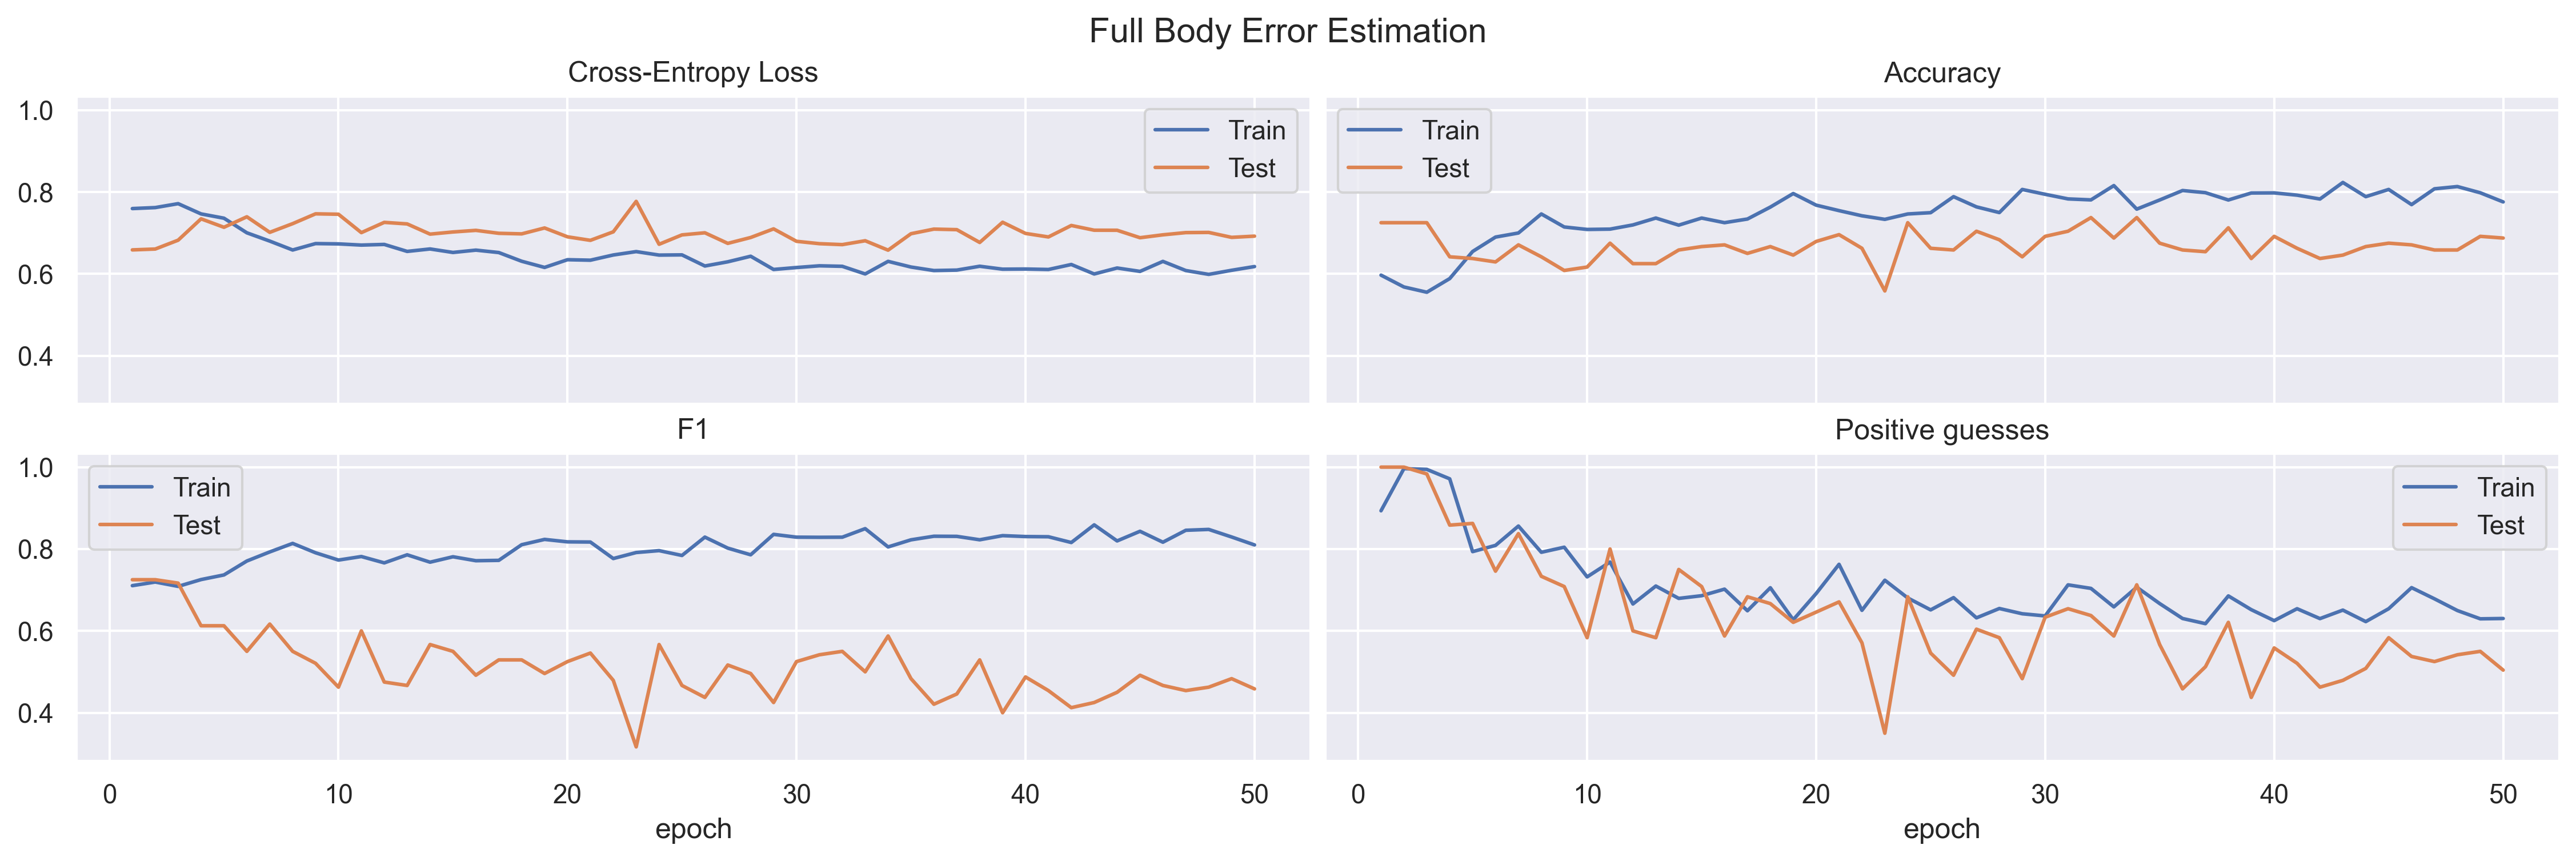
\includegraphics[width=0.8\textwidth]{figures/Results/v1/fb/FullBody_ErrorEstimation.png}
  \caption[Full Body model training results]{The training results of the Full Body model.}
  \label{fig:full_body_training_results_v1}
\end{figure}

\begin{figure}[htbp]
  \centering
  \begin{subfigure}[b]{0.8\textwidth}
      \centering
      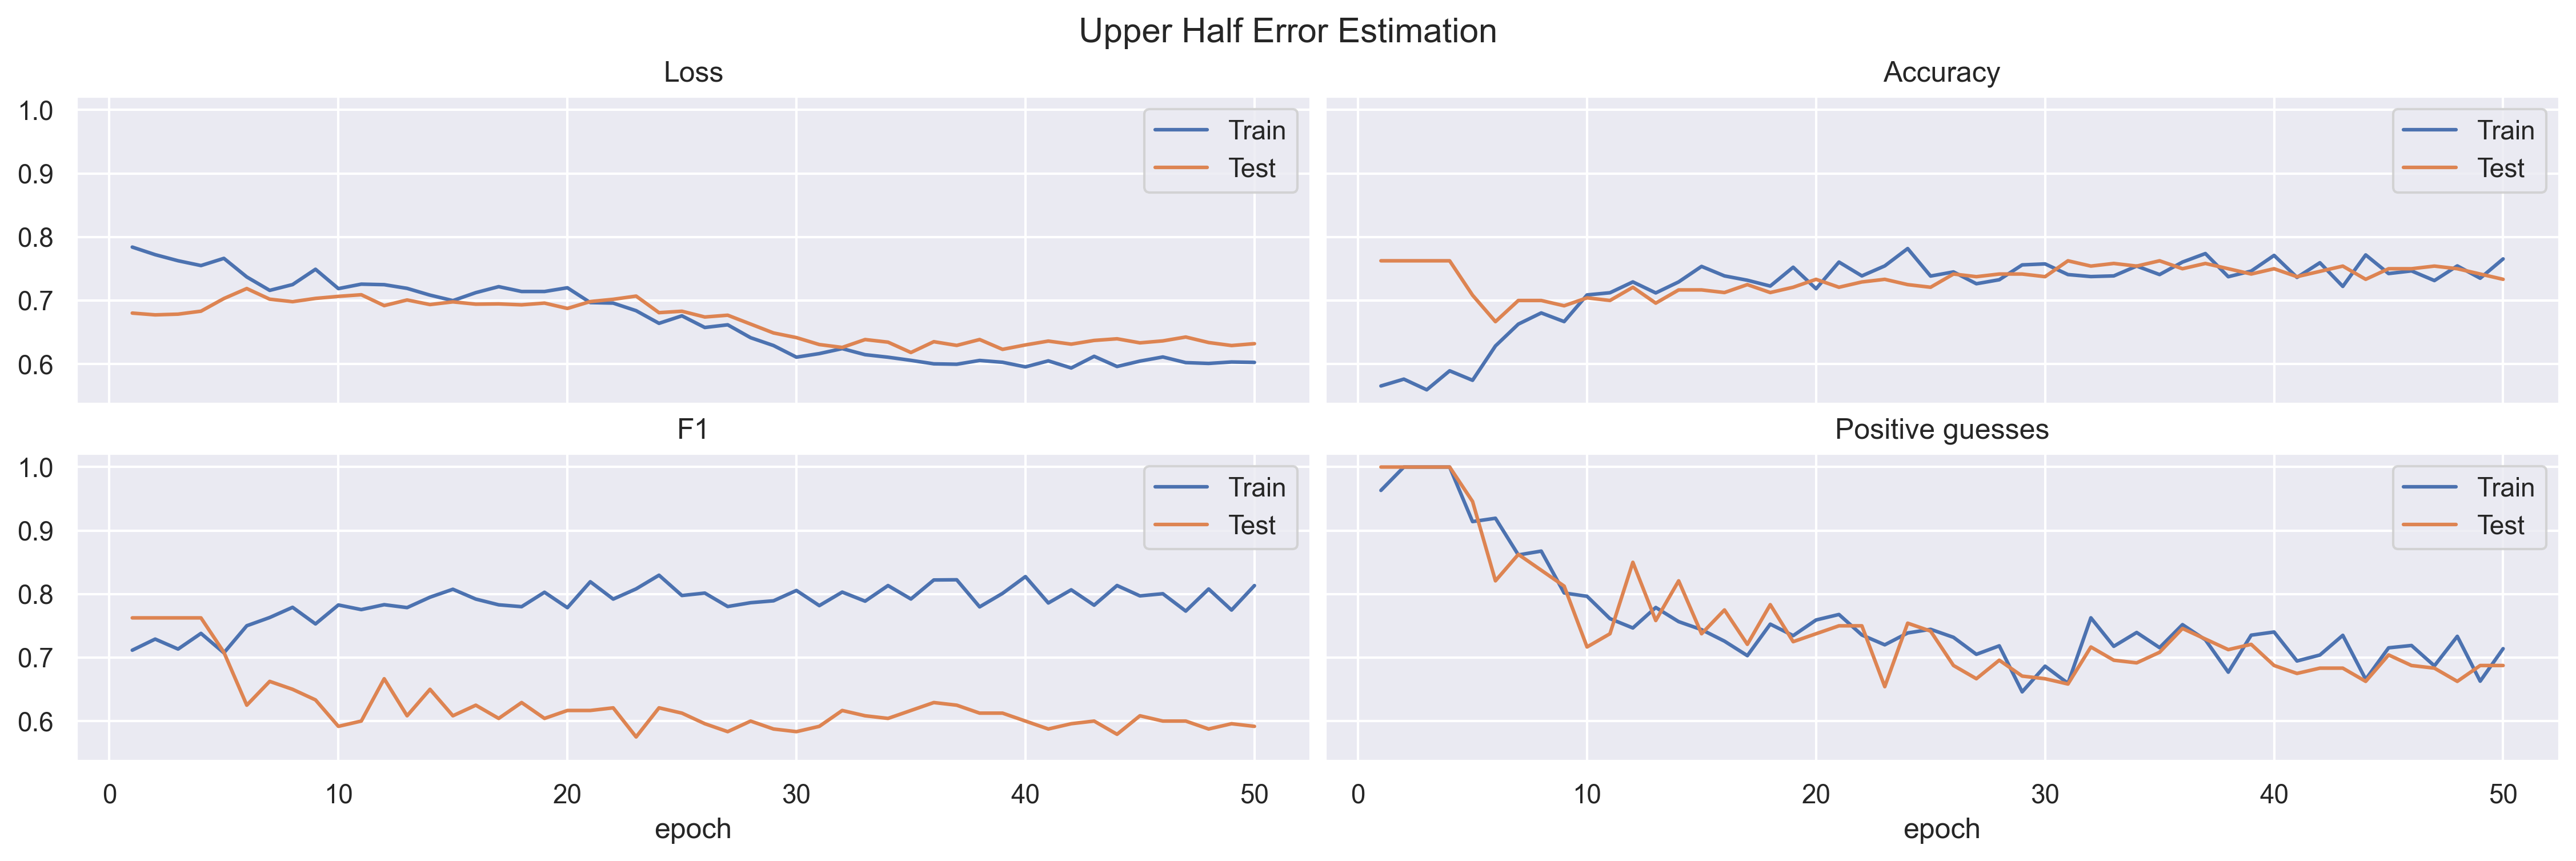
\includegraphics[width=\textwidth]{figures/Results/v1/hb/UpperBody_ErrorEstimation.png}
      \caption{Upper Body Error Estimation}
      \label{fig:uh_ee}
  \end{subfigure}
  \hfill
  \begin{subfigure}[b]{0.8\textwidth}
      \centering
      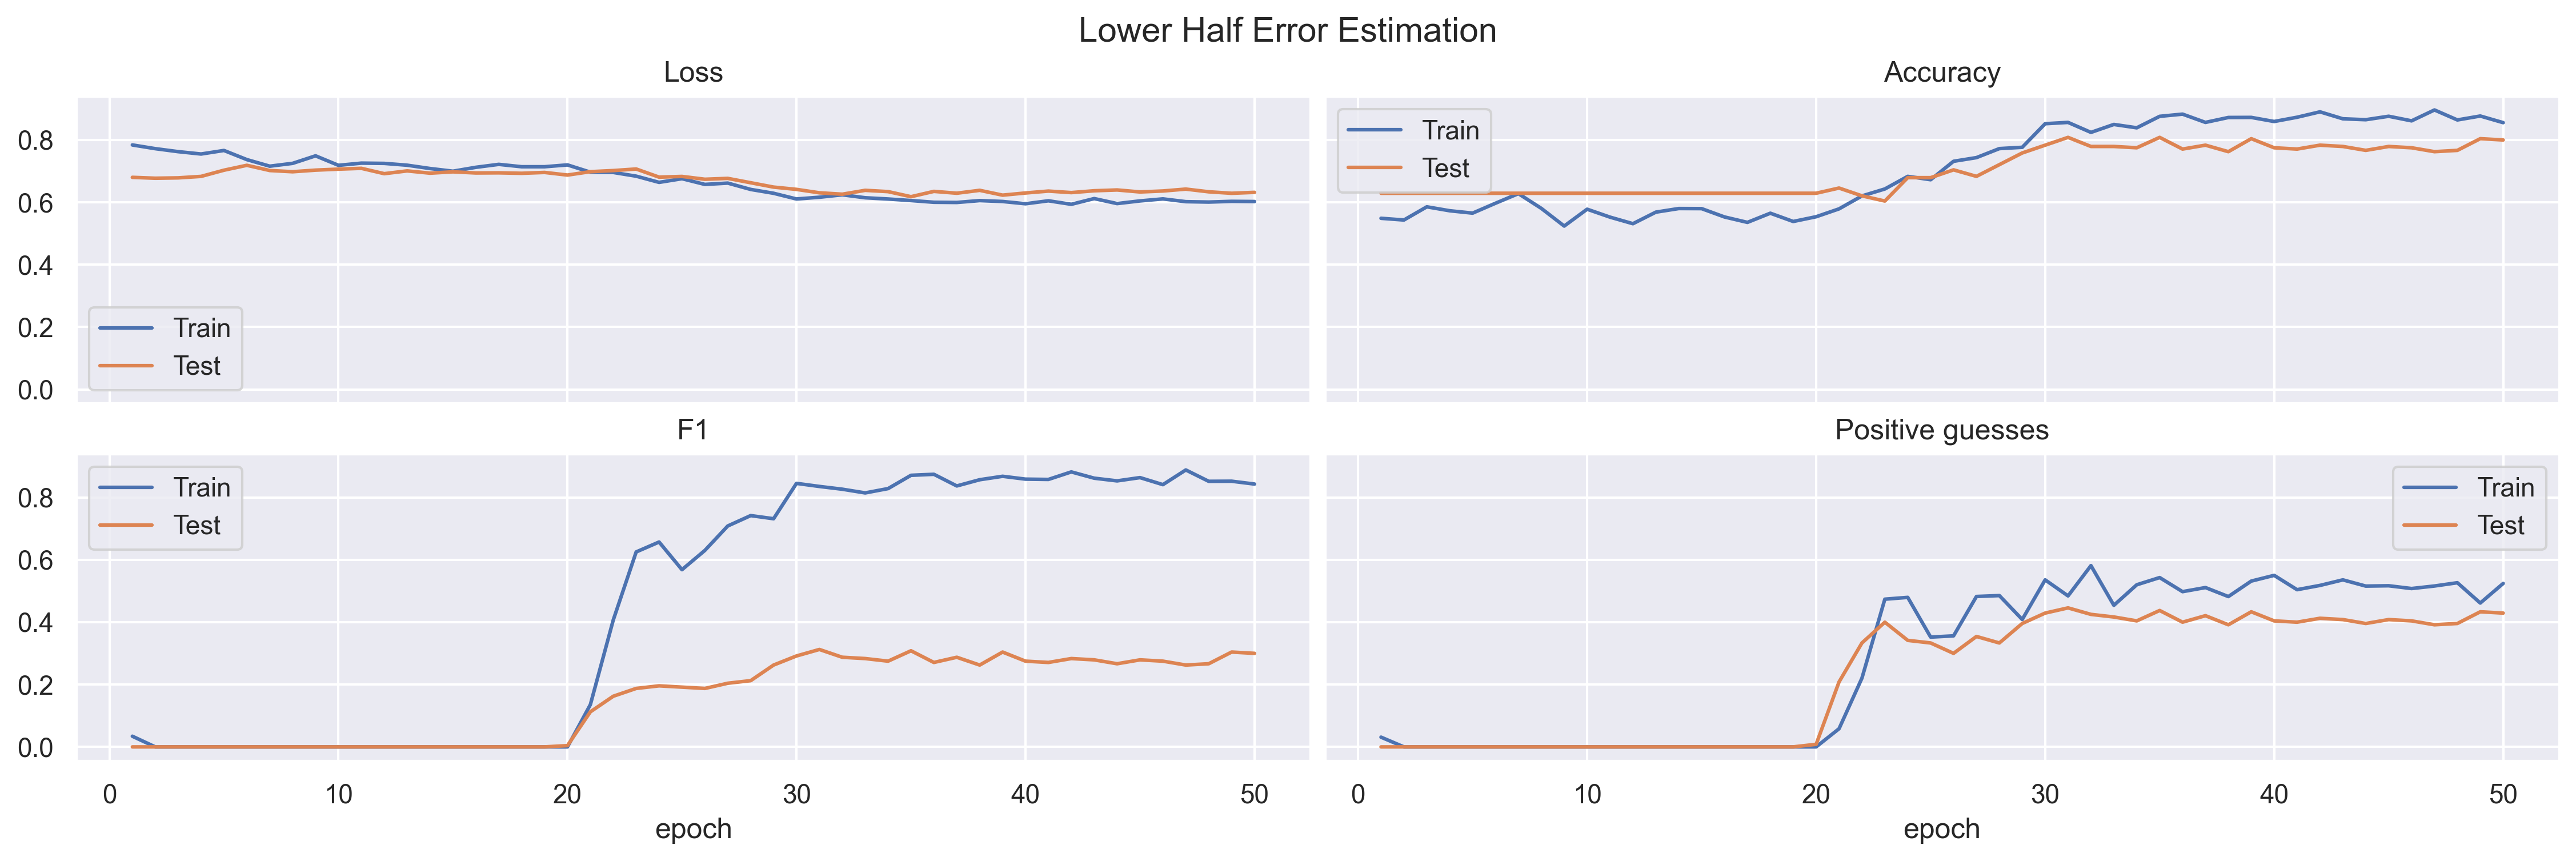
\includegraphics[width=\textwidth]{figures/Results/v1/hb/LowerBody_ErrorEstimation.png}
      \caption{Lower Body Error Estimation}
      \label{fig:lh_ee}
  \end{subfigure}
  \caption[Half Body model training results]{The training results of the Half Body error estimation model.}
     \label{fig:half_body_training_results}
\end{figure}

\begin{figure}[htbp]
  \centering
  \begin{subfigure}[b]{0.9\linewidth}
      \centering
      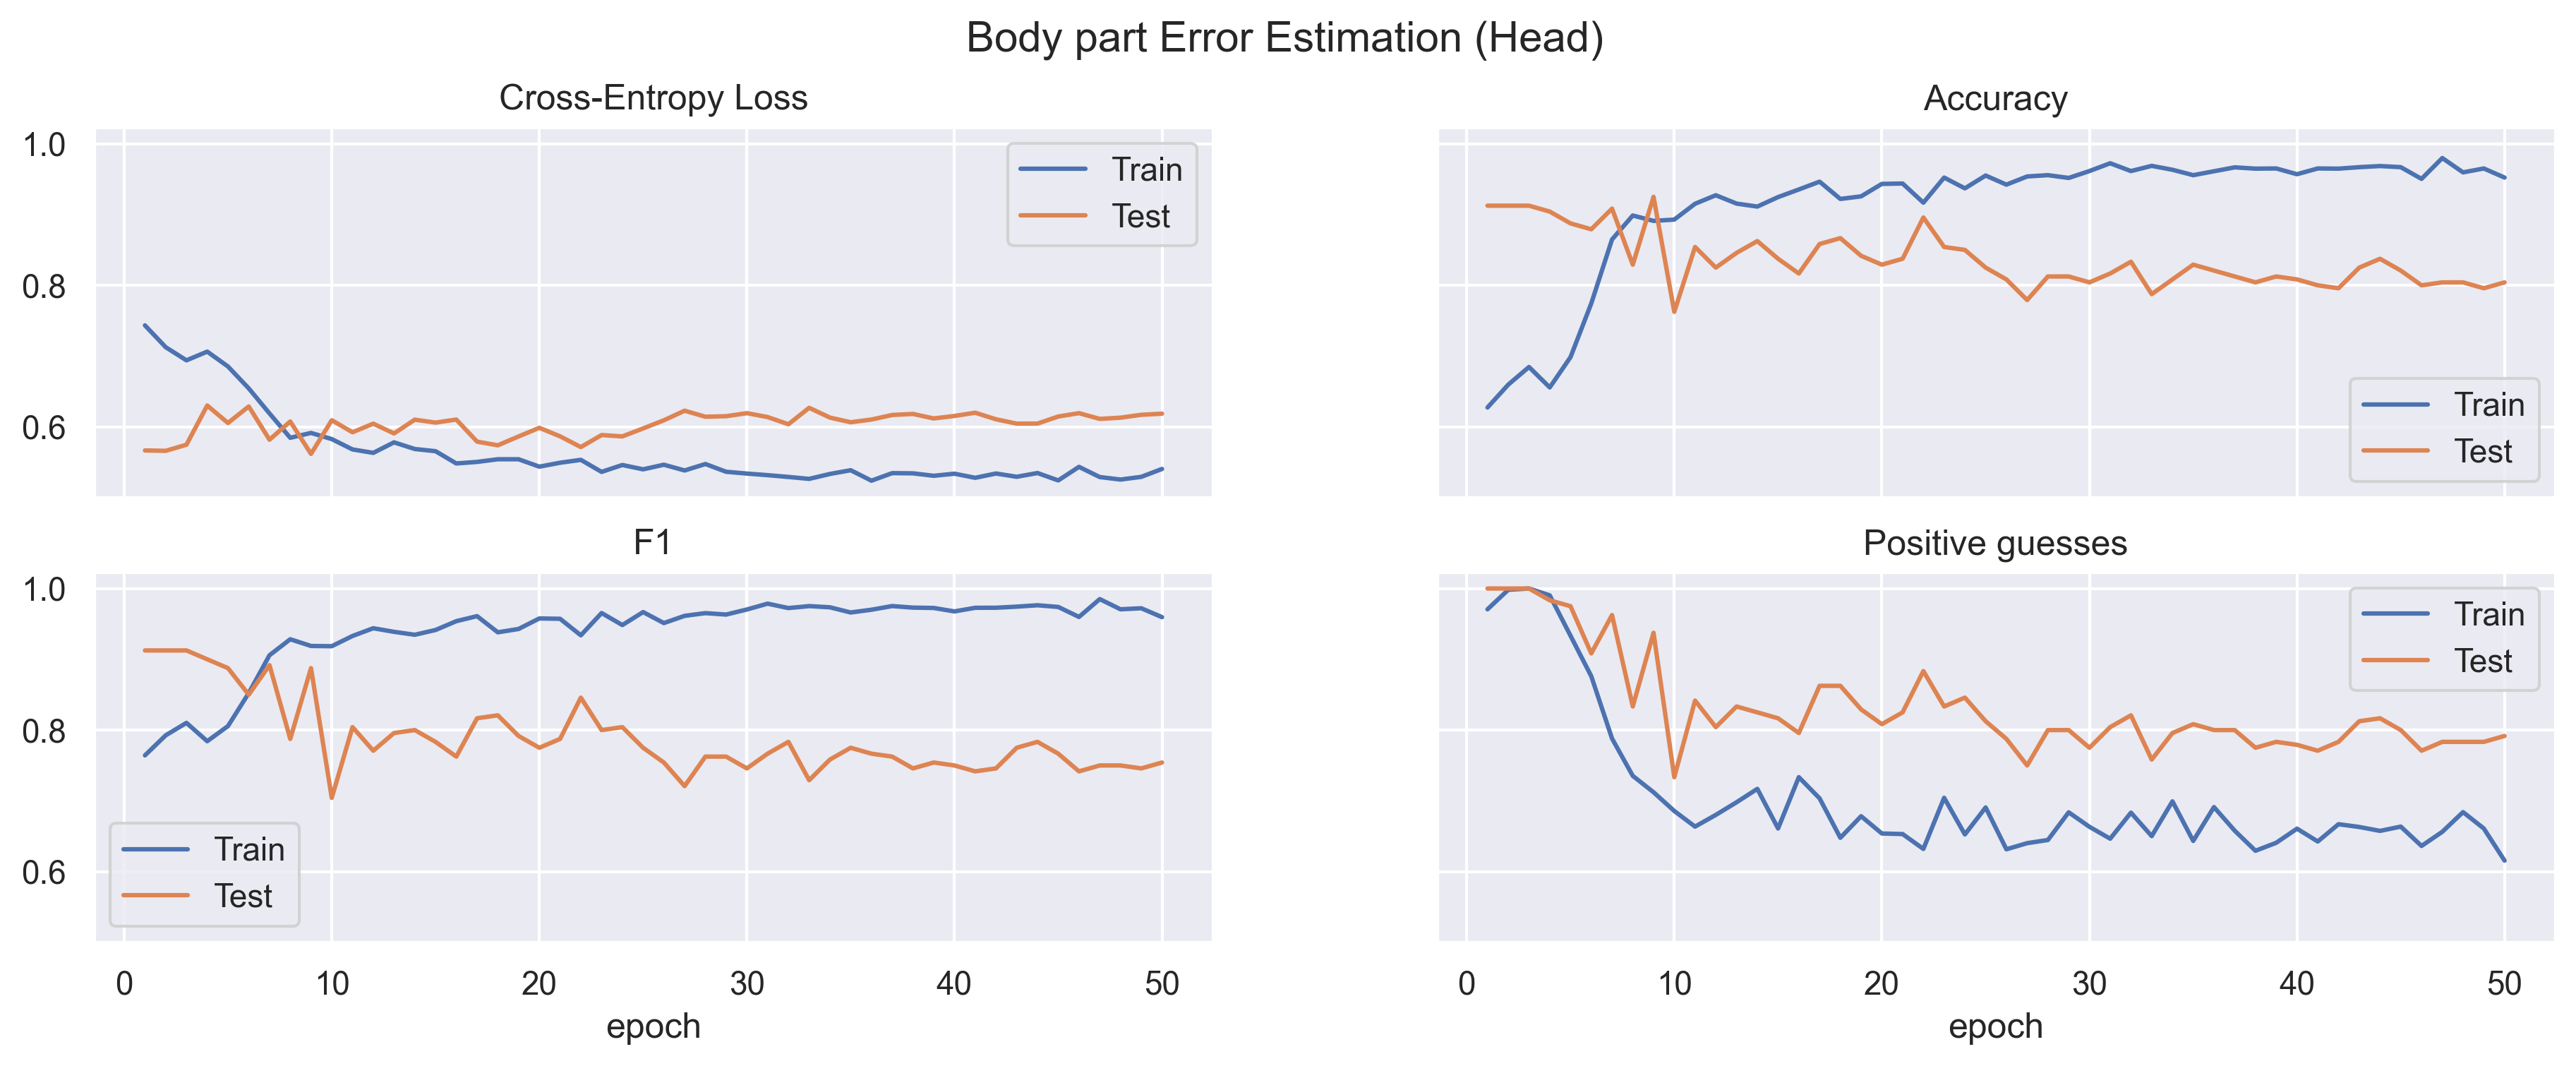
\includegraphics[width=\textwidth]{figures/Results/v1/bp/Head_ErrorEstimation.png}
      \caption{Head Error Estimation}
      \label{fig:head_lb_ee}
  \end{subfigure}
  \hfill
  \begin{subfigure}[b]{0.9\linewidth}
      \centering
      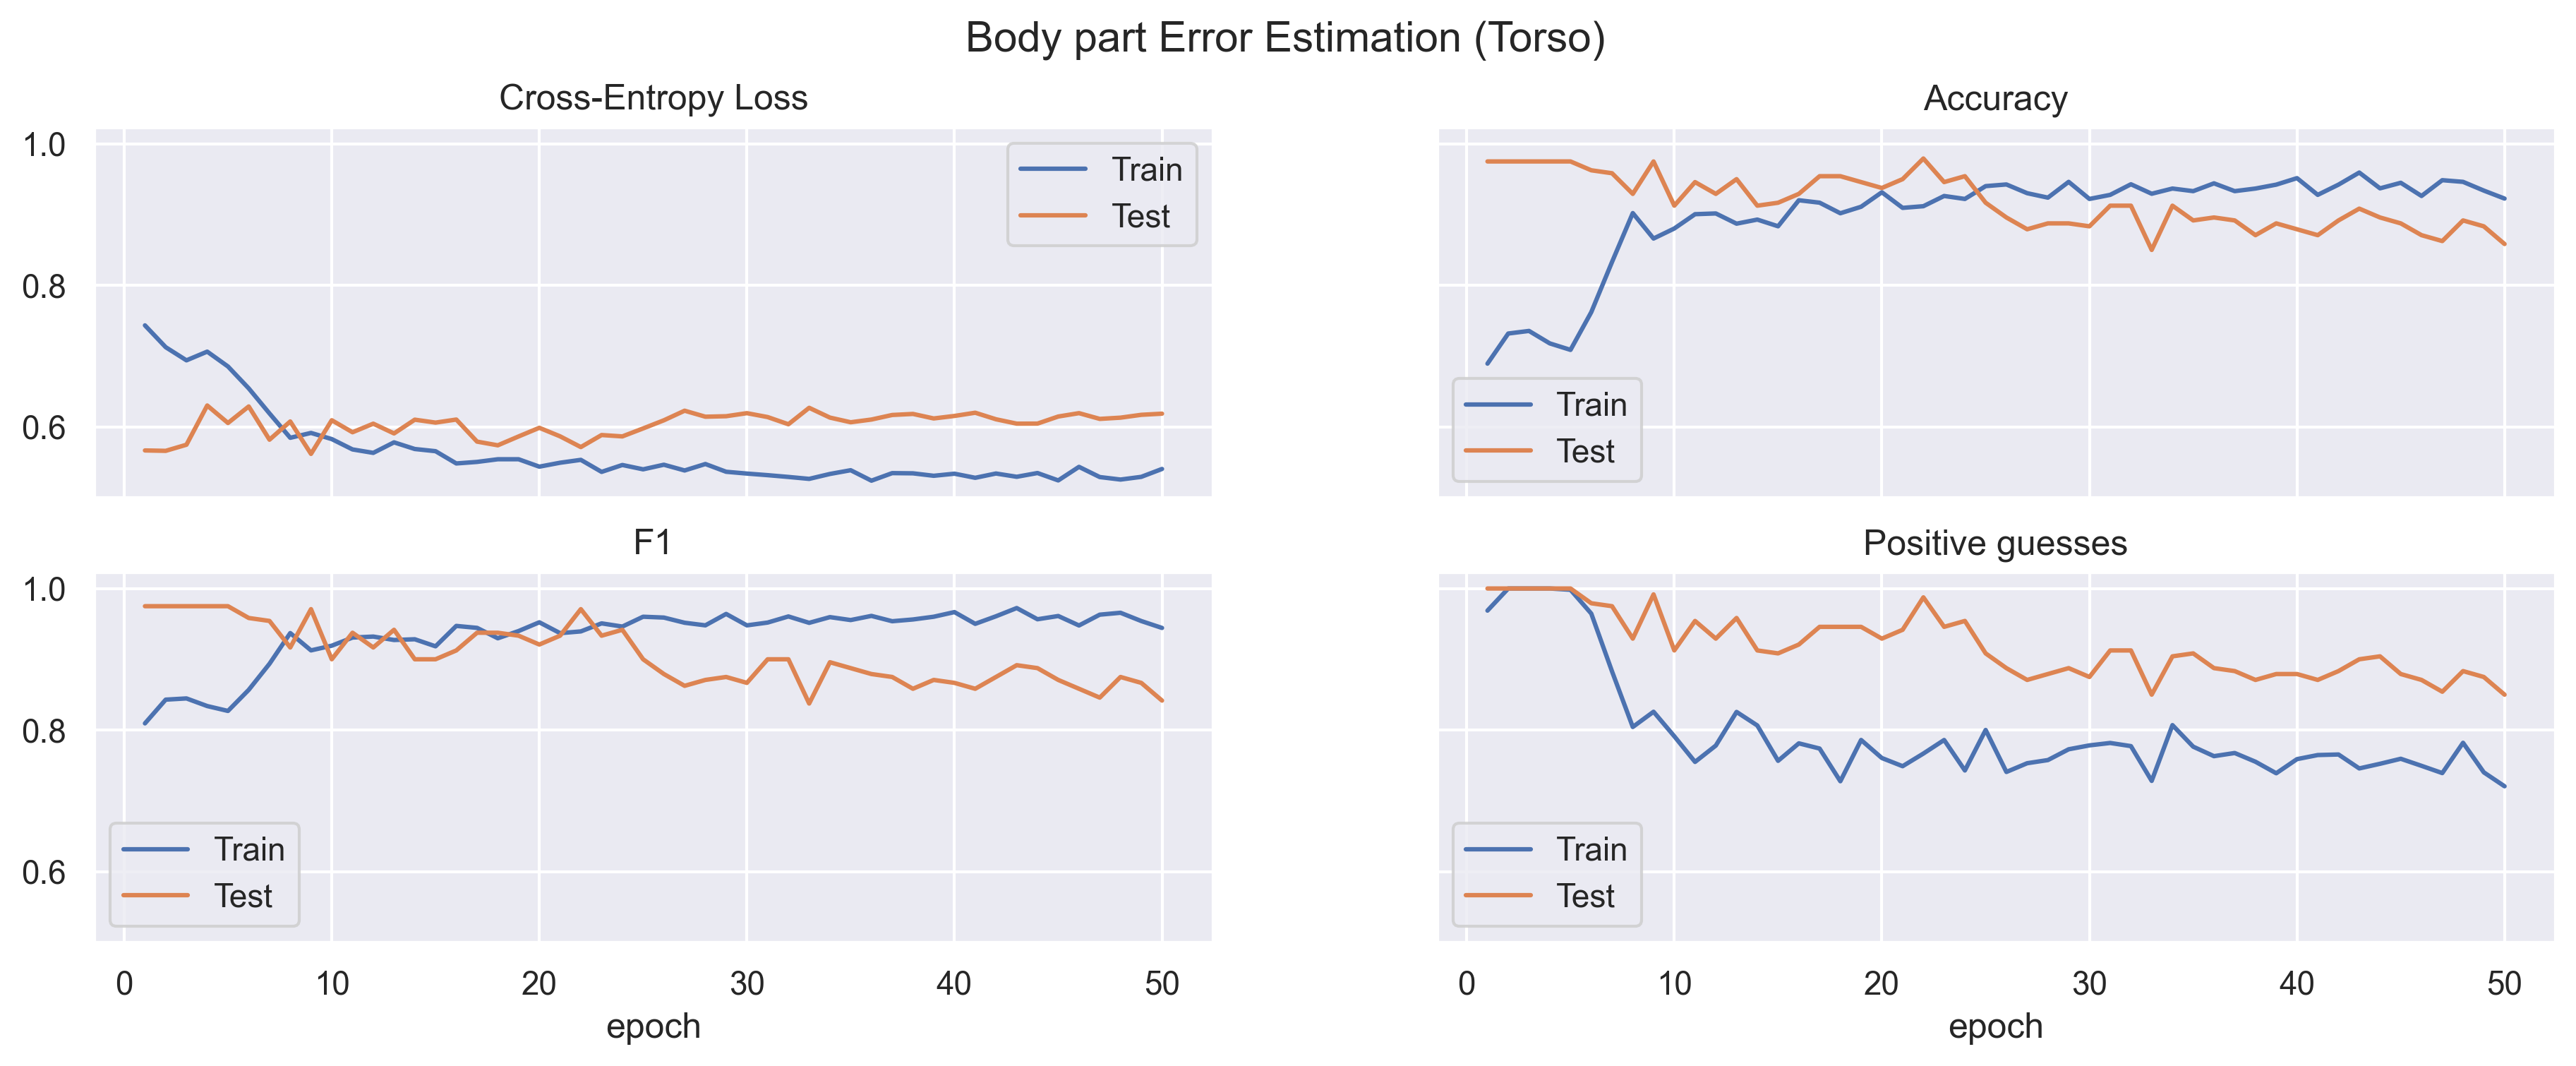
\includegraphics[width=\textwidth]{figures/Results/v1/bp/Torso_ErrorEstimation.png}
      \caption{Torso Error Estimation}
      \label{fig:torso_lb_ee}
  \end{subfigure}
  \hfill
  \begin{subfigure}[b]{0.9\linewidth}
      \centering
      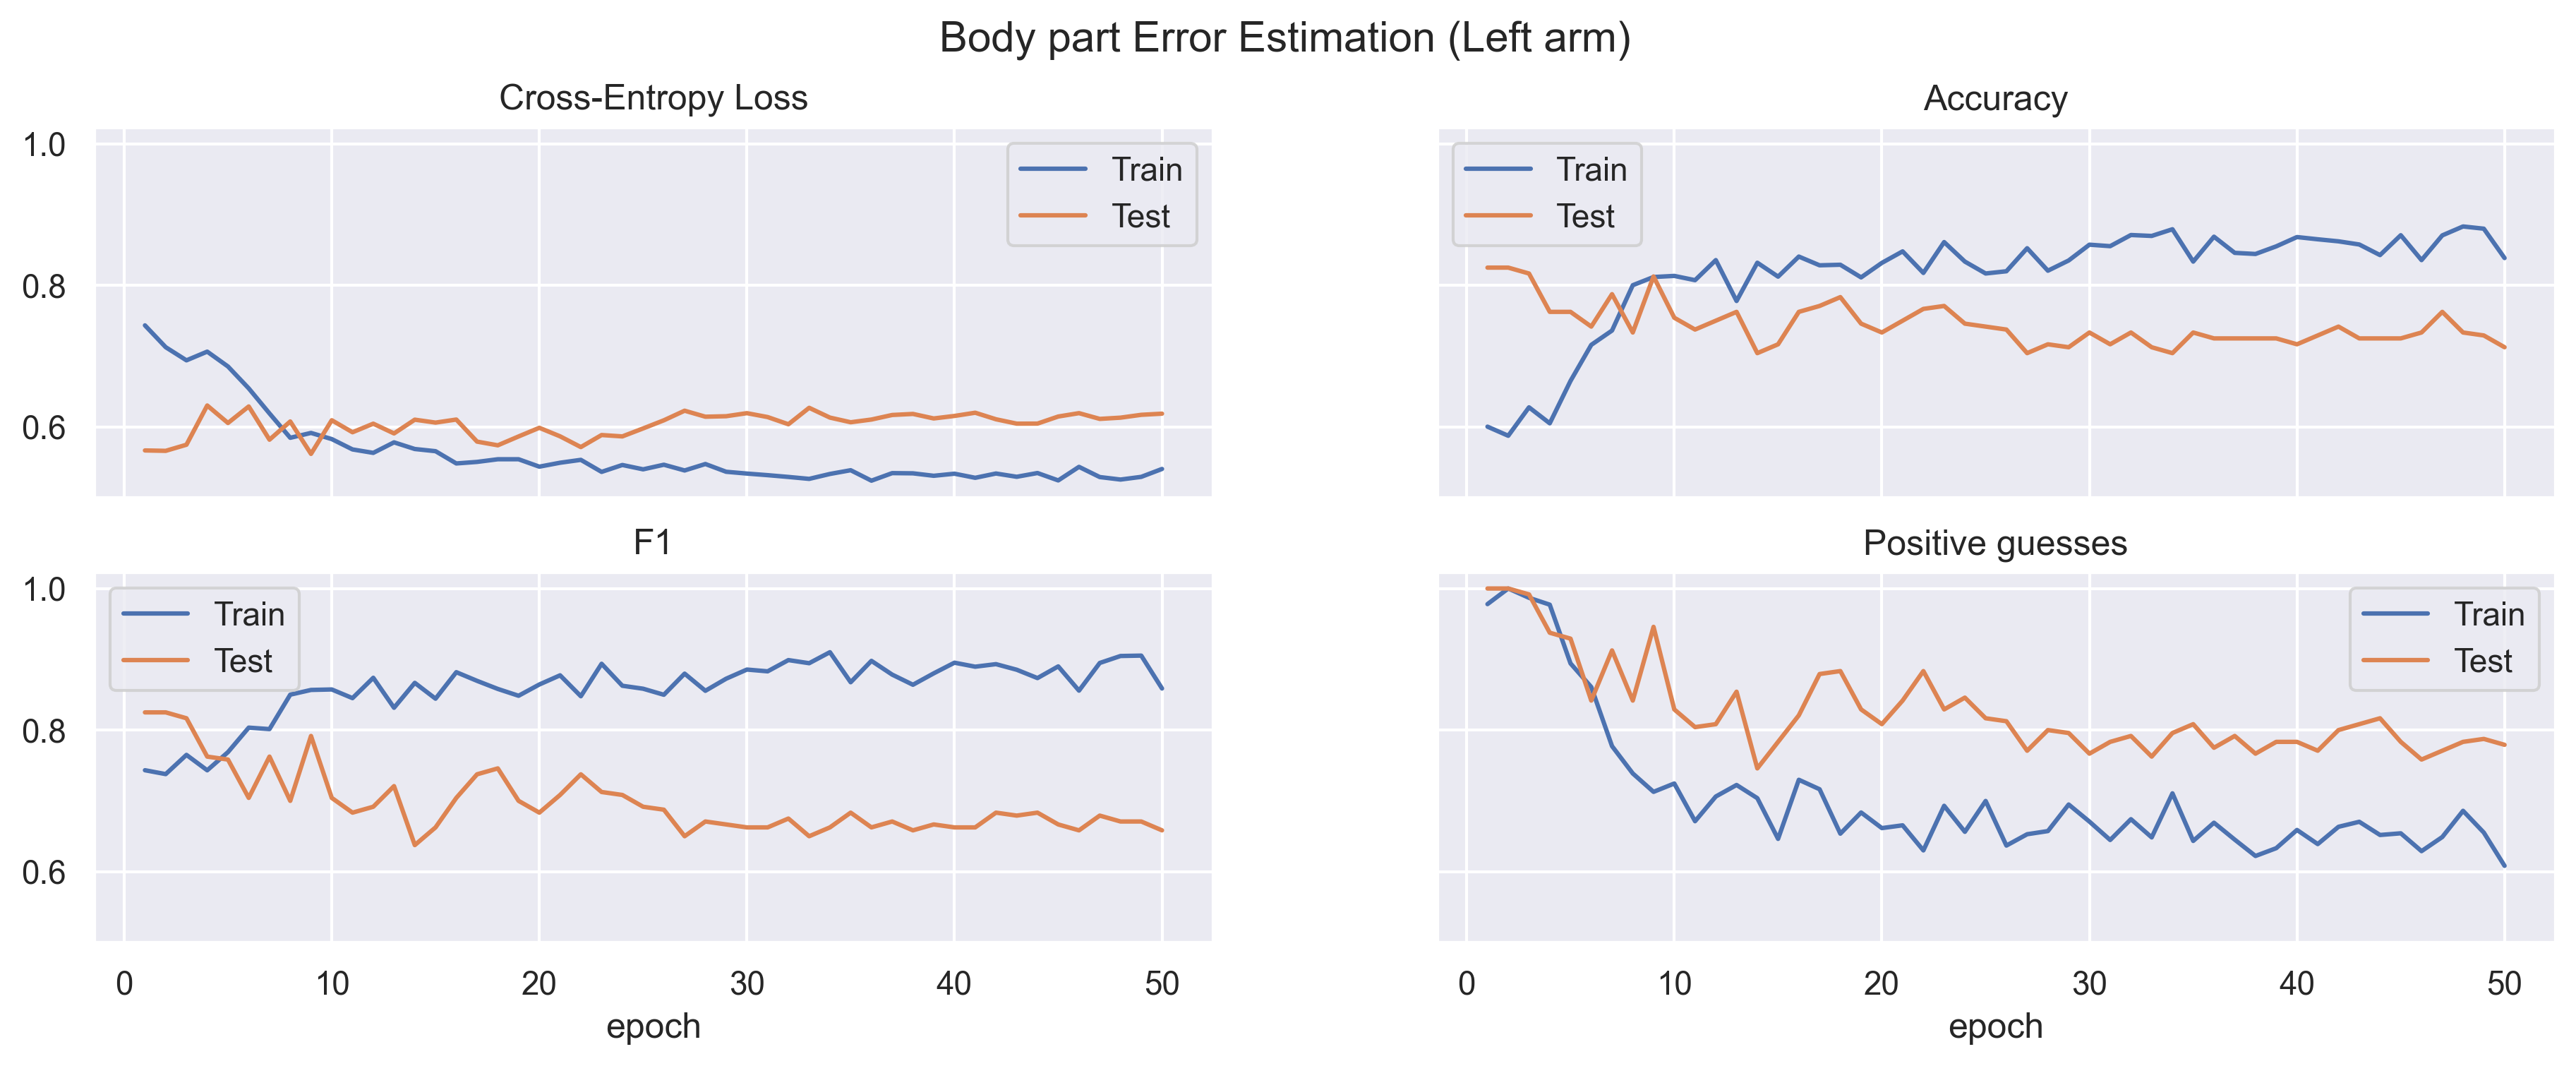
\includegraphics[width=\textwidth]{figures/Results/v1/bp/Left arm_ErrorEstimation.png}
      \caption{Left Arm Error Estimation}
      \label{fig:lear_lb_ee}
  \end{subfigure}
\end{figure}


\begin{figure}[htbp]
  \begin{subfigure}[b]{0.9\linewidth}
      \centering
      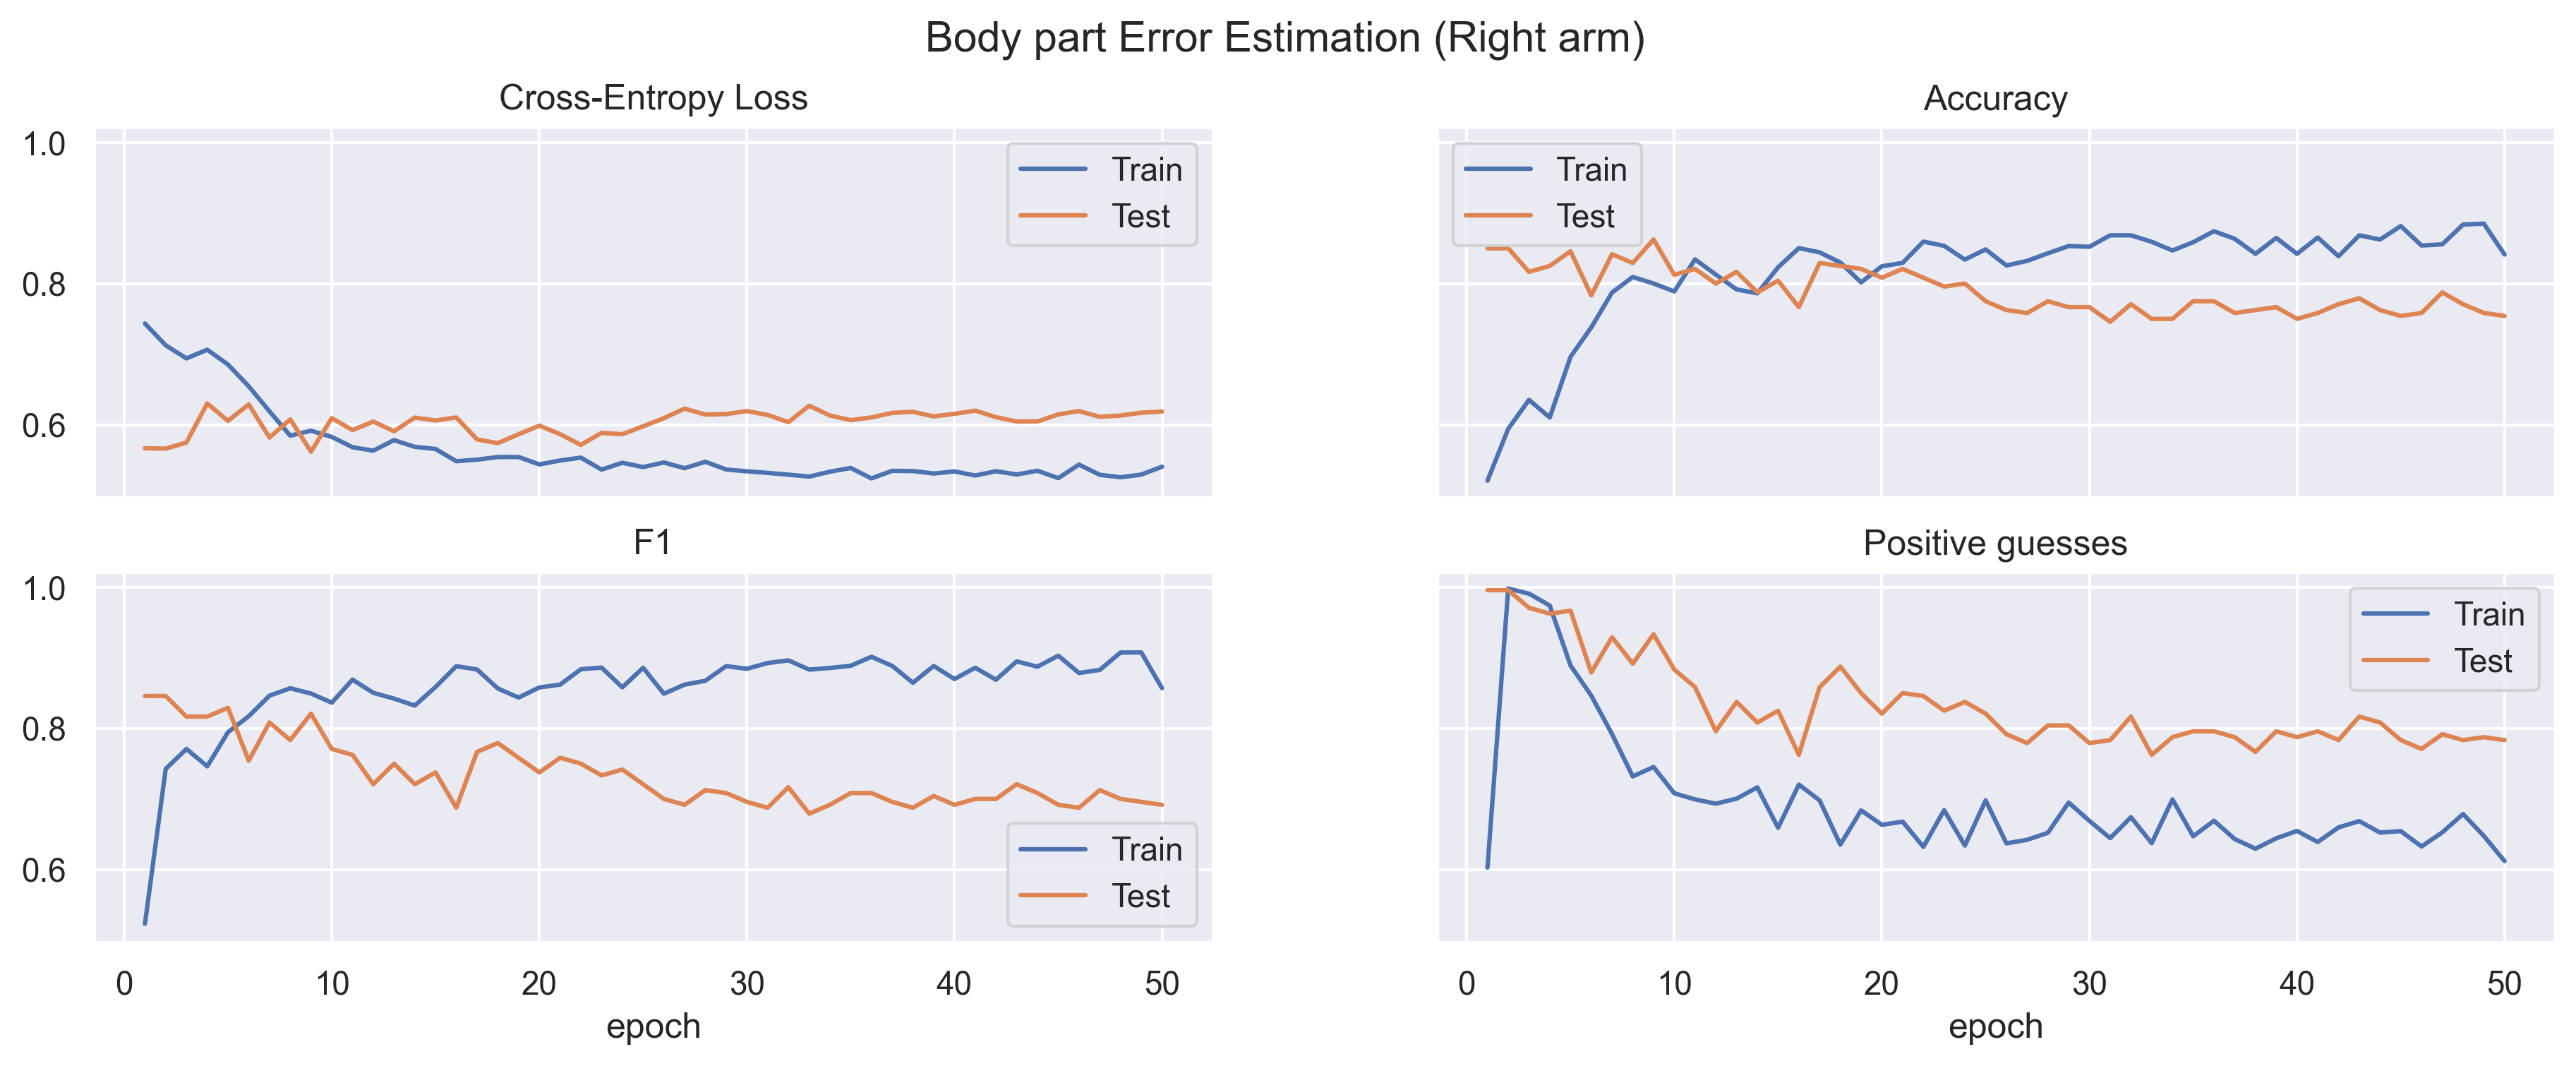
\includegraphics[width=\textwidth]{figures/Results/v1/bp/Right arm_ErrorEstimation.png}
      \caption{Right Arm Error Estimation}
      \label{fig:riar_lb_ee}
  \end{subfigure}
  \hfill
  \begin{subfigure}[b]{0.9\linewidth}
      \centering
      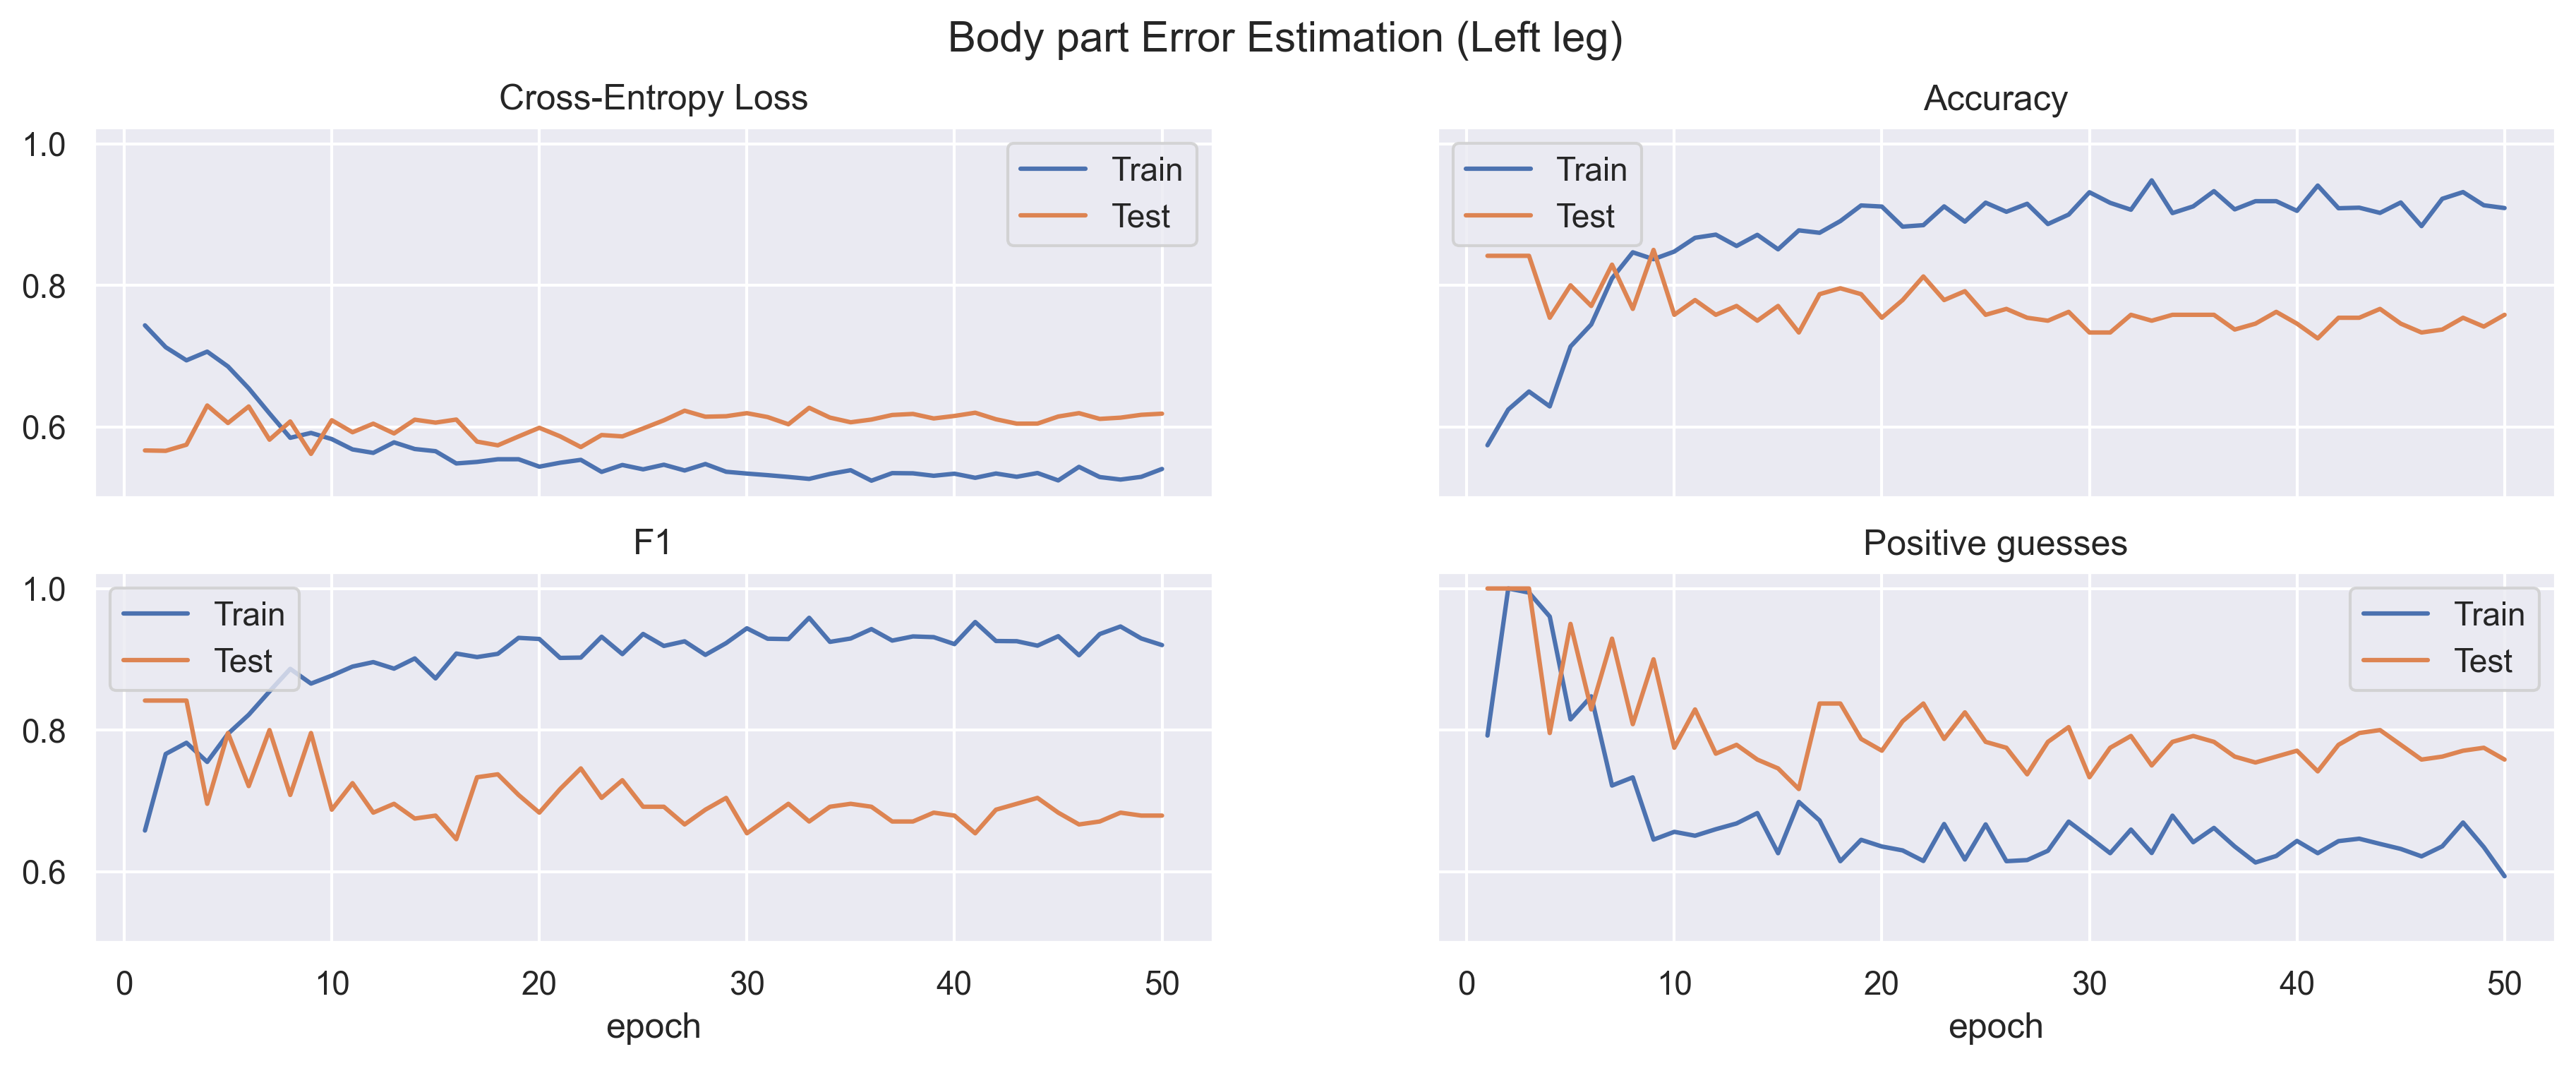
\includegraphics[width=\textwidth]{figures/Results/v1/bp/Left leg_ErrorEstimation.png}
      \caption{Left leg Error Estimation}
      \label{fig:lele_lb_ee}
  \end{subfigure}
  \hfill
  \begin{subfigure}[b]{0.9\linewidth}
      \centering
      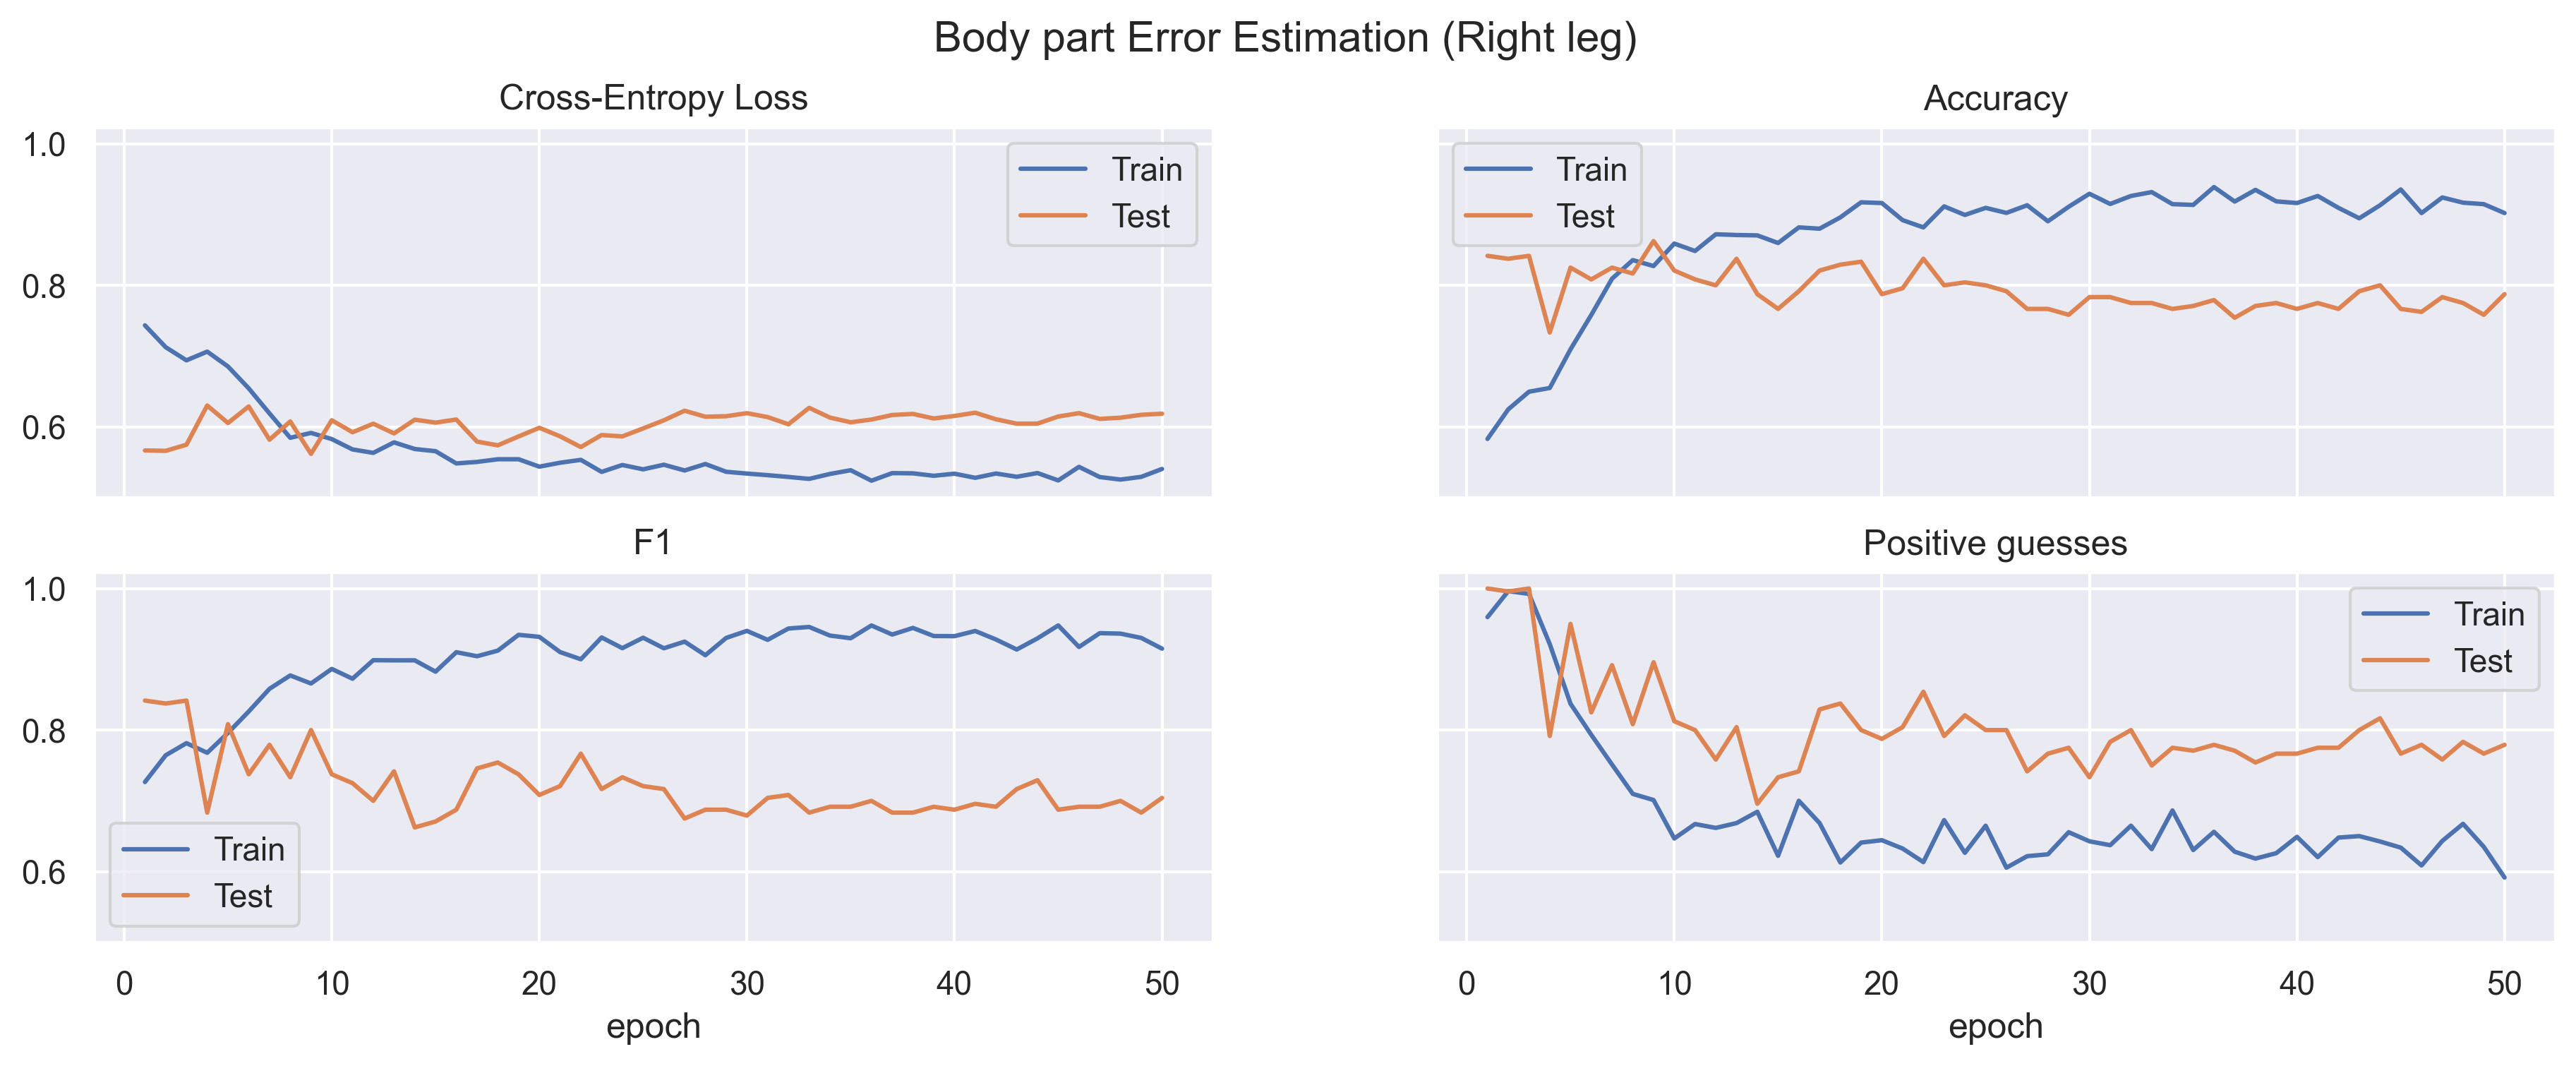
\includegraphics[width=\textwidth]{figures/Results/v1/bp/Right leg_ErrorEstimation.png}
      \caption{Right leg Error Estimation}
      \label{fig:rileg_lb_ee}
  \end{subfigure}
  \hfill
  \caption[Body Parts model training results]{The training results of the body part error estimation model.}
  \label{fig:body part_training_results}
\end{figure}

\begin{figure}[!ht]
  \centering
  \begin{subfigure}[b]{0.47\linewidth}
      \centering
      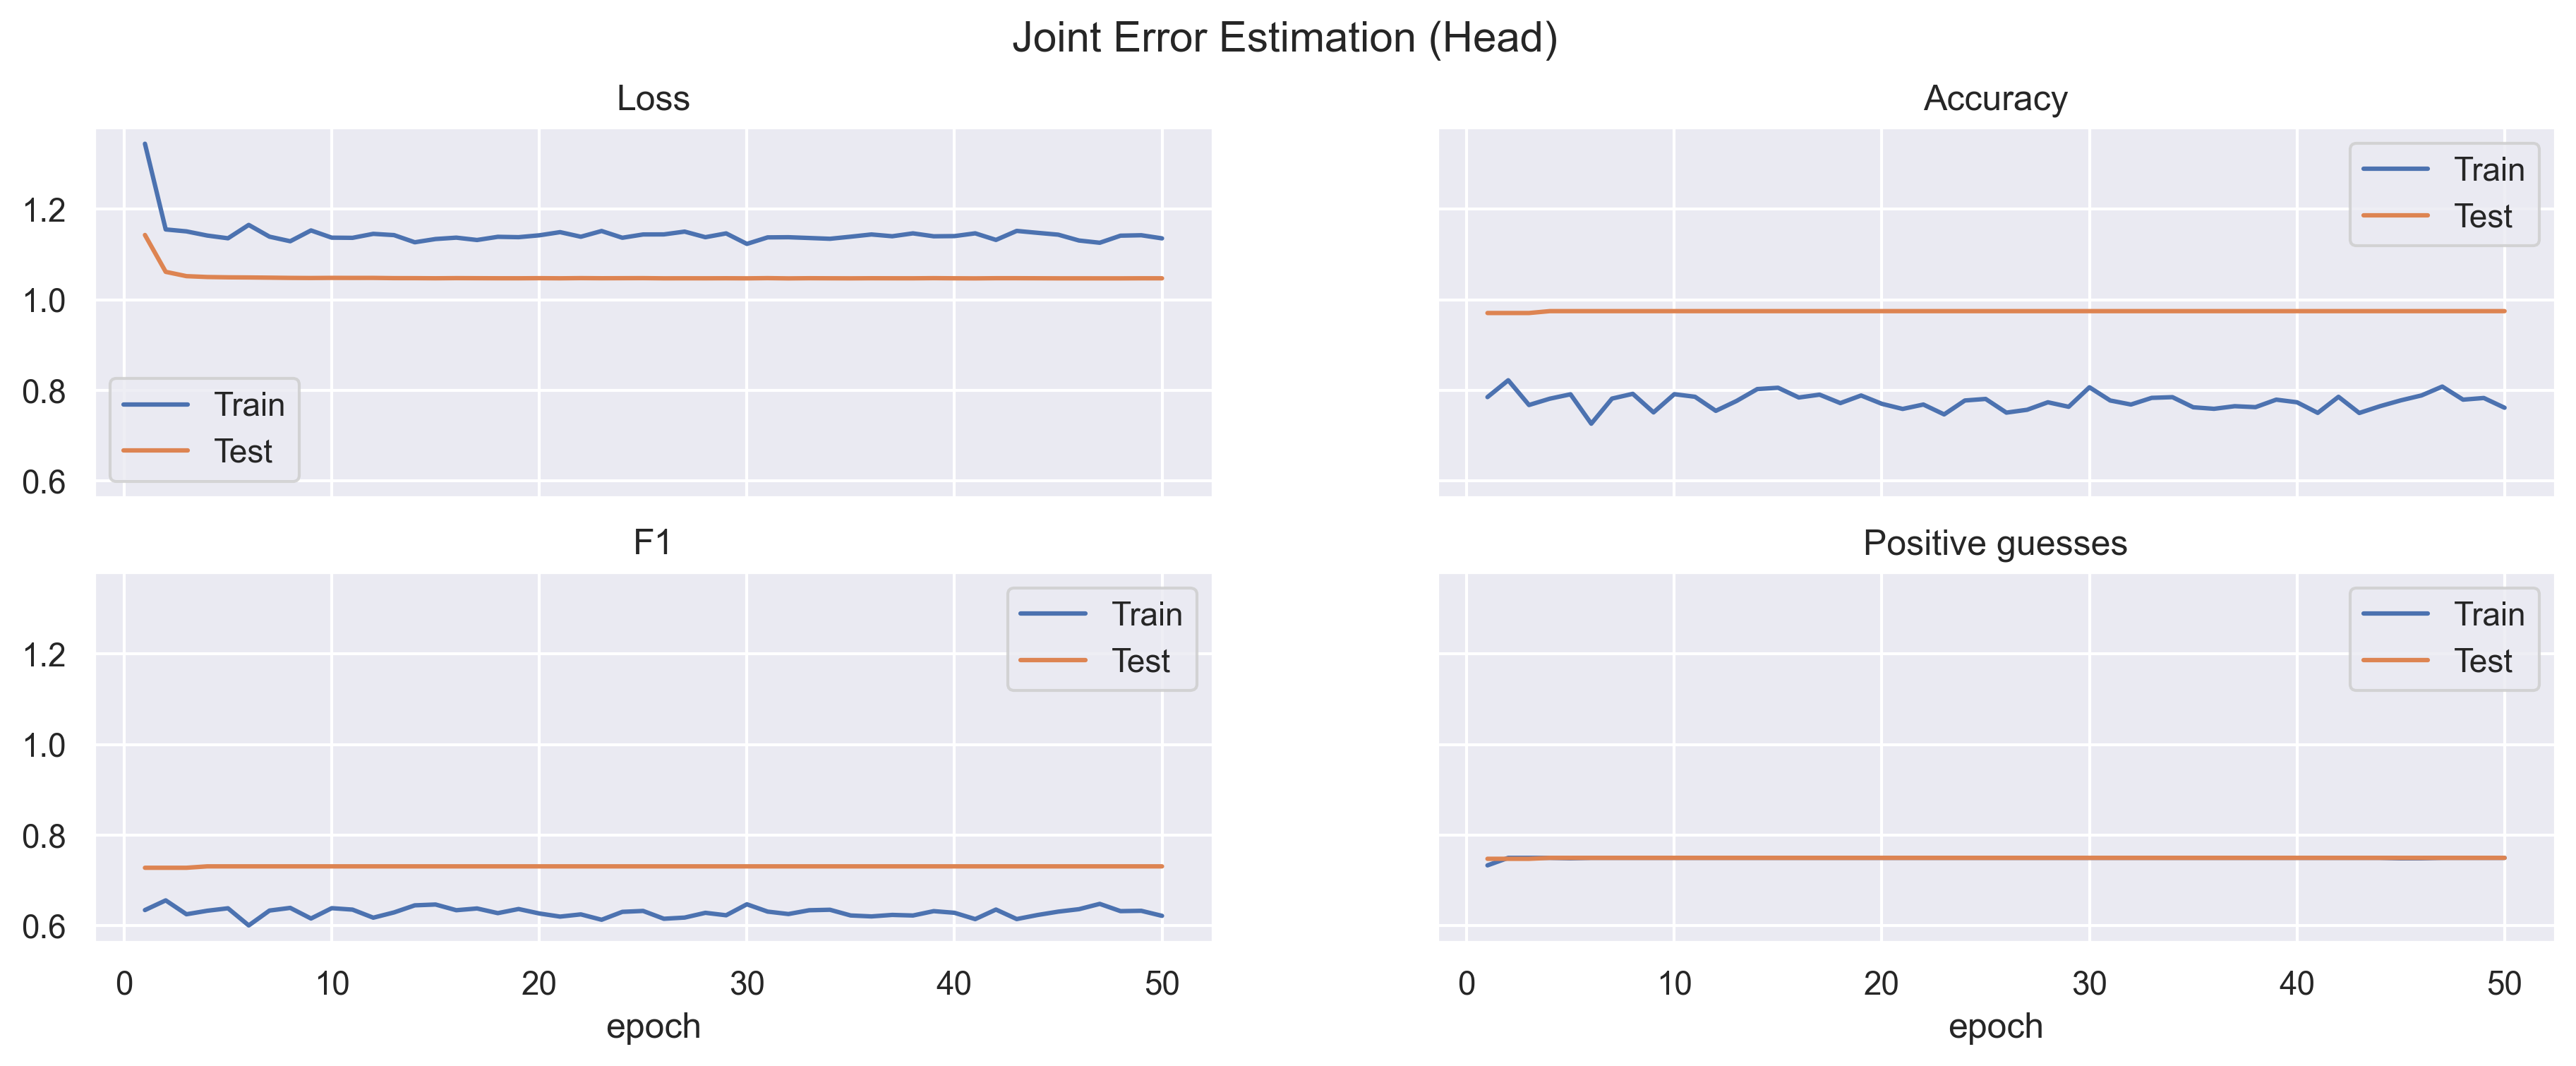
\includegraphics[width=\textwidth]{figures/Results/v1_bs_60_is_64_e_100/jt/Head_ErrorEstimation.png}
      \caption{Head Error Estimation}
      \label{fig:v1_head_jt_ee}
  \end{subfigure}
  \hfill
  \begin{subfigure}[b]{0.47\linewidth}
      \centering
      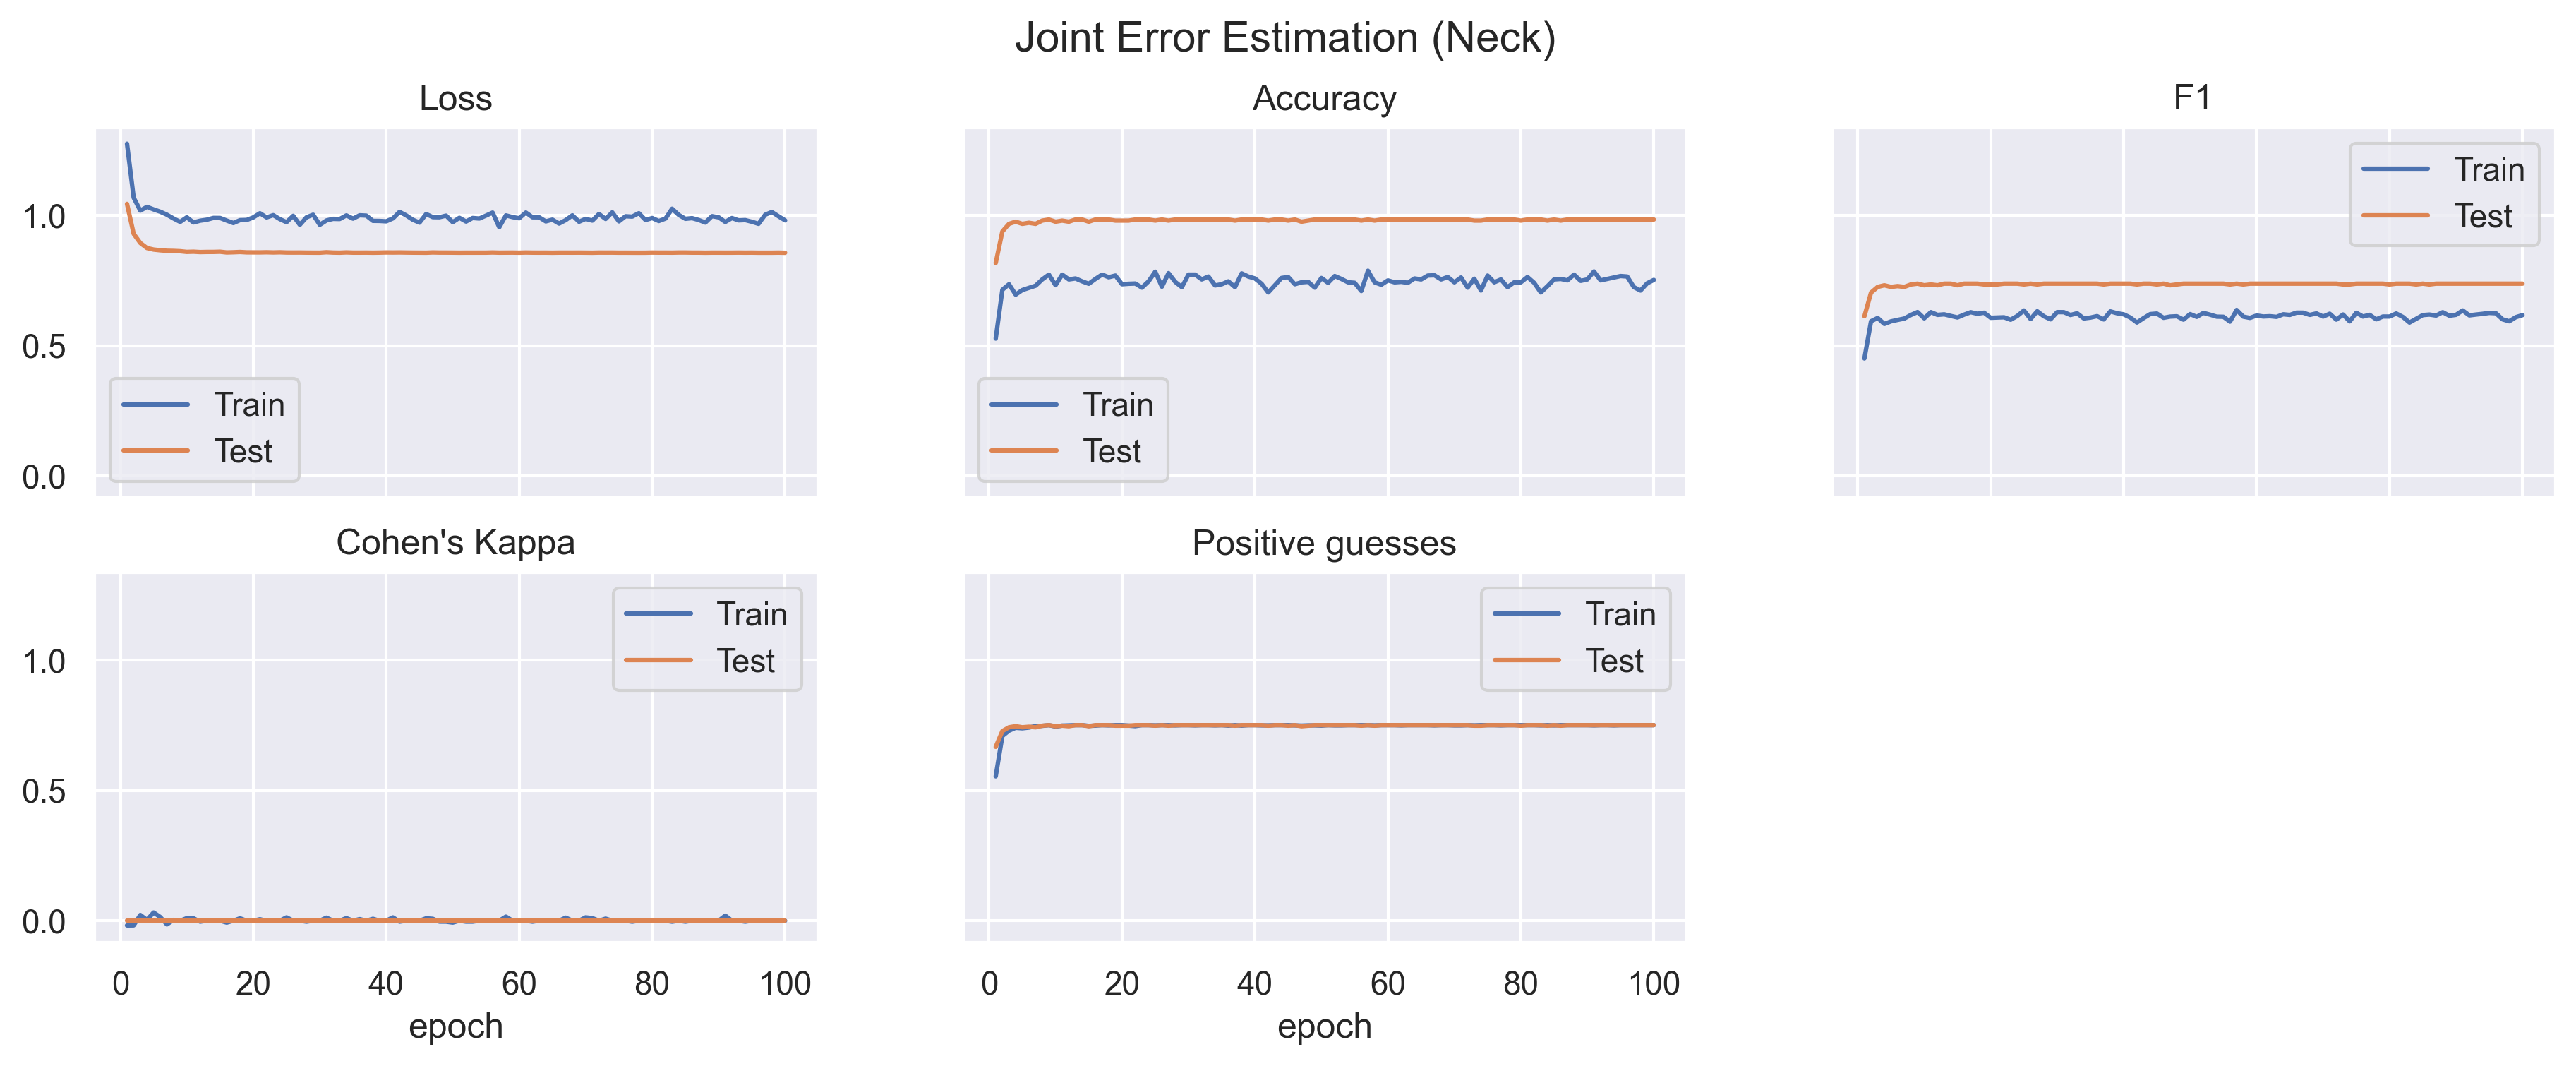
\includegraphics[width=\textwidth]{figures/Results/v1_bs_60_is_64_e_100/jt/Neck_ErrorEstimation.png}
      \caption{Neck Error Estimation}
      \label{fig:v1_neck_jt_ee}
  \end{subfigure}
  \hfill
  \begin{subfigure}[b]{0.47\linewidth}
      \centering
      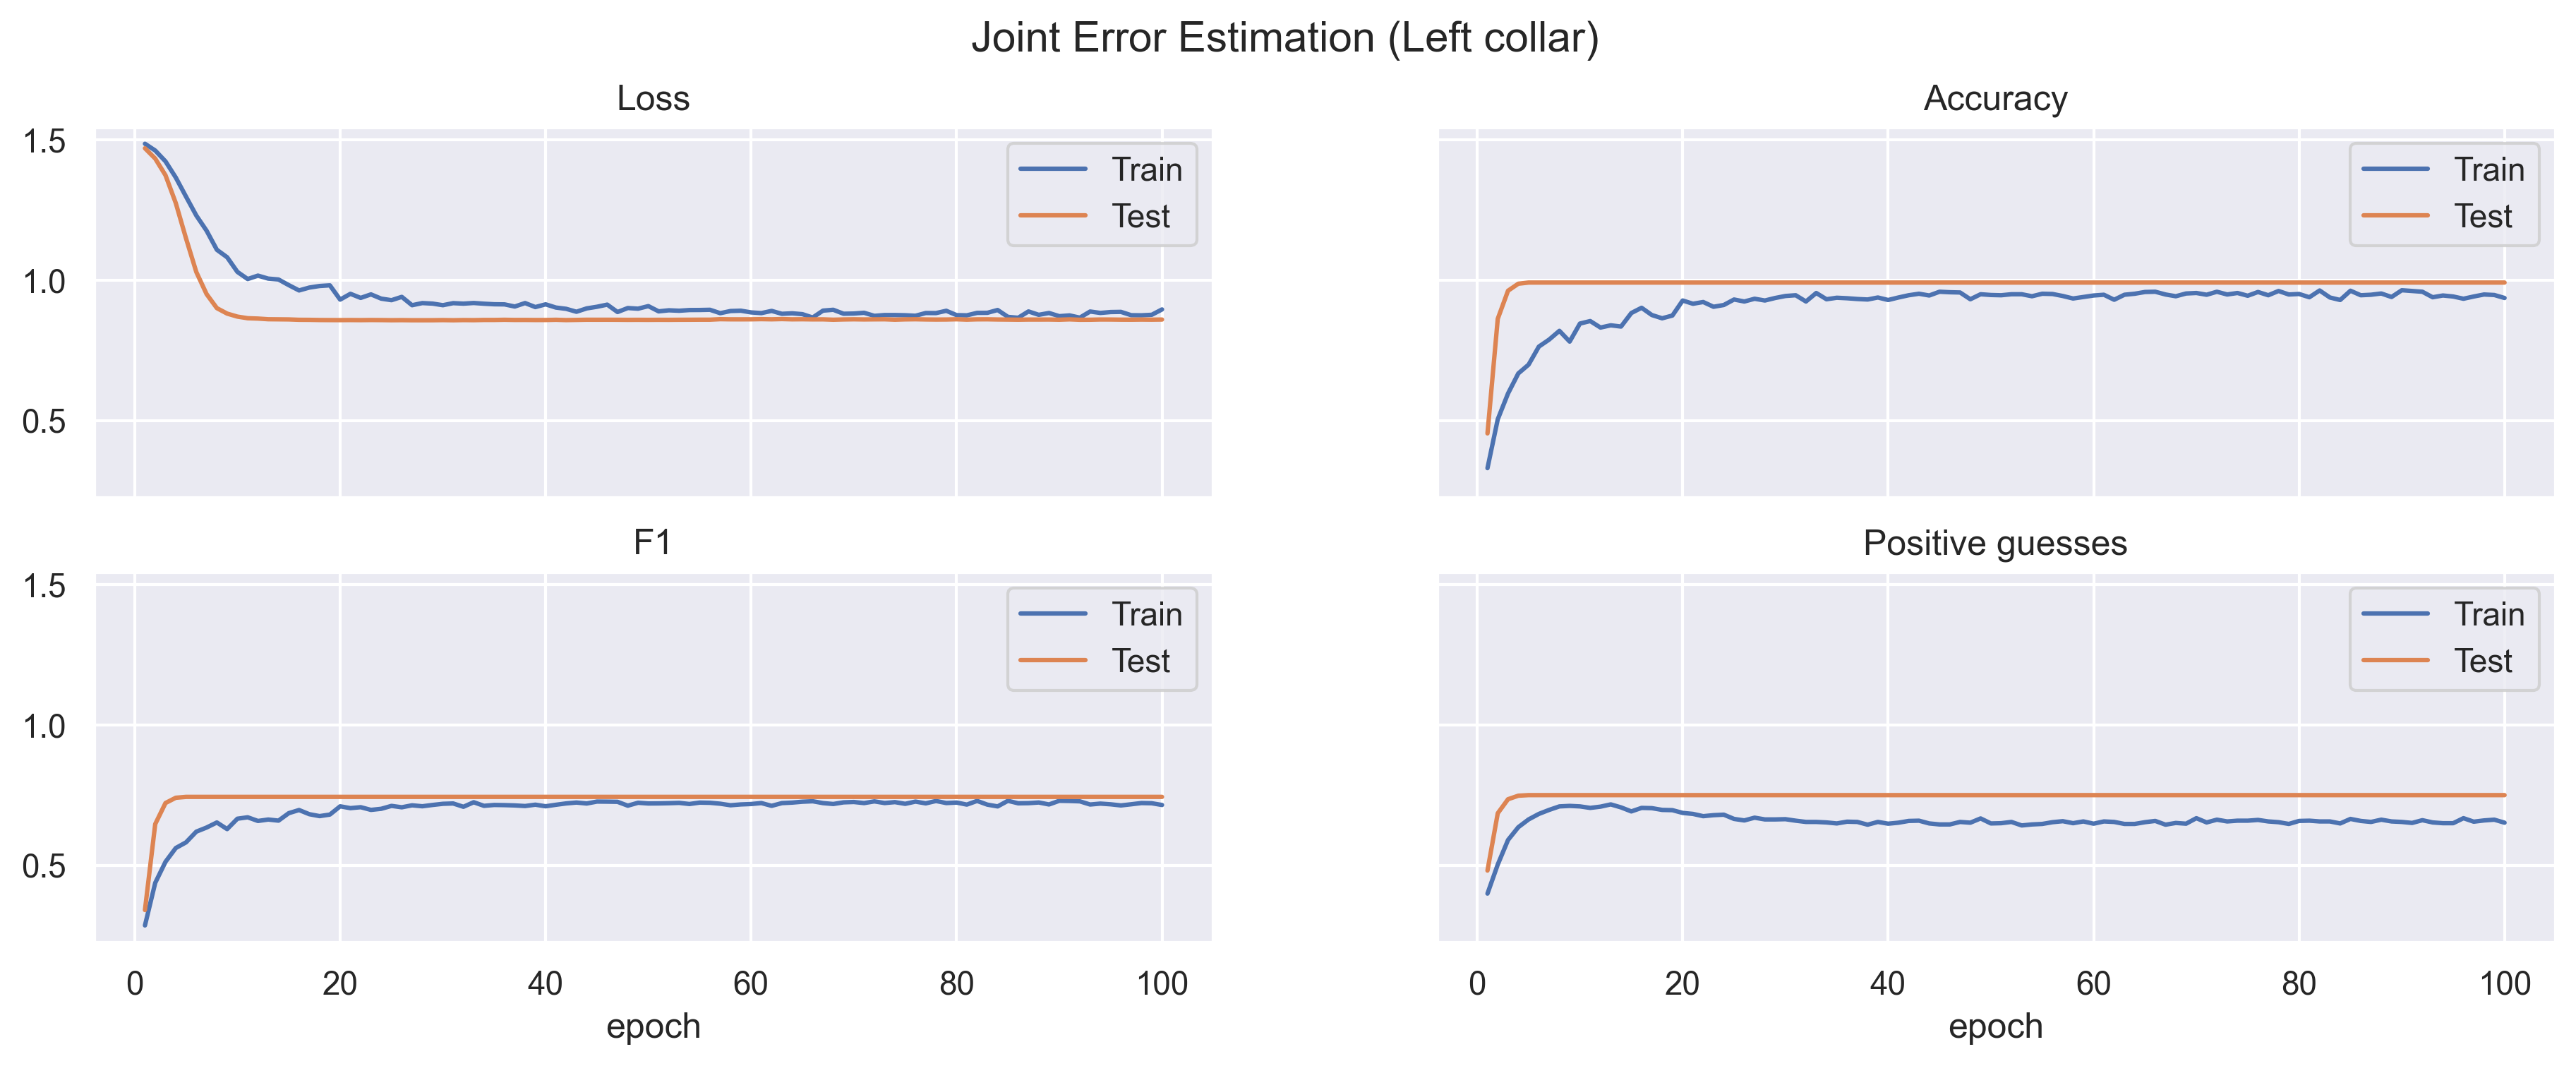
\includegraphics[width=\textwidth]{figures/Results/v1_bs_60_is_64_e_100/jt/Left collar_ErrorEstimation.png}
      \caption{Left Collar Error Estimation}
      \label{fig:v1_leco_jt_ee}
  \end{subfigure}
  \hfill
  \begin{subfigure}[b]{0.47\linewidth}
      \centering
      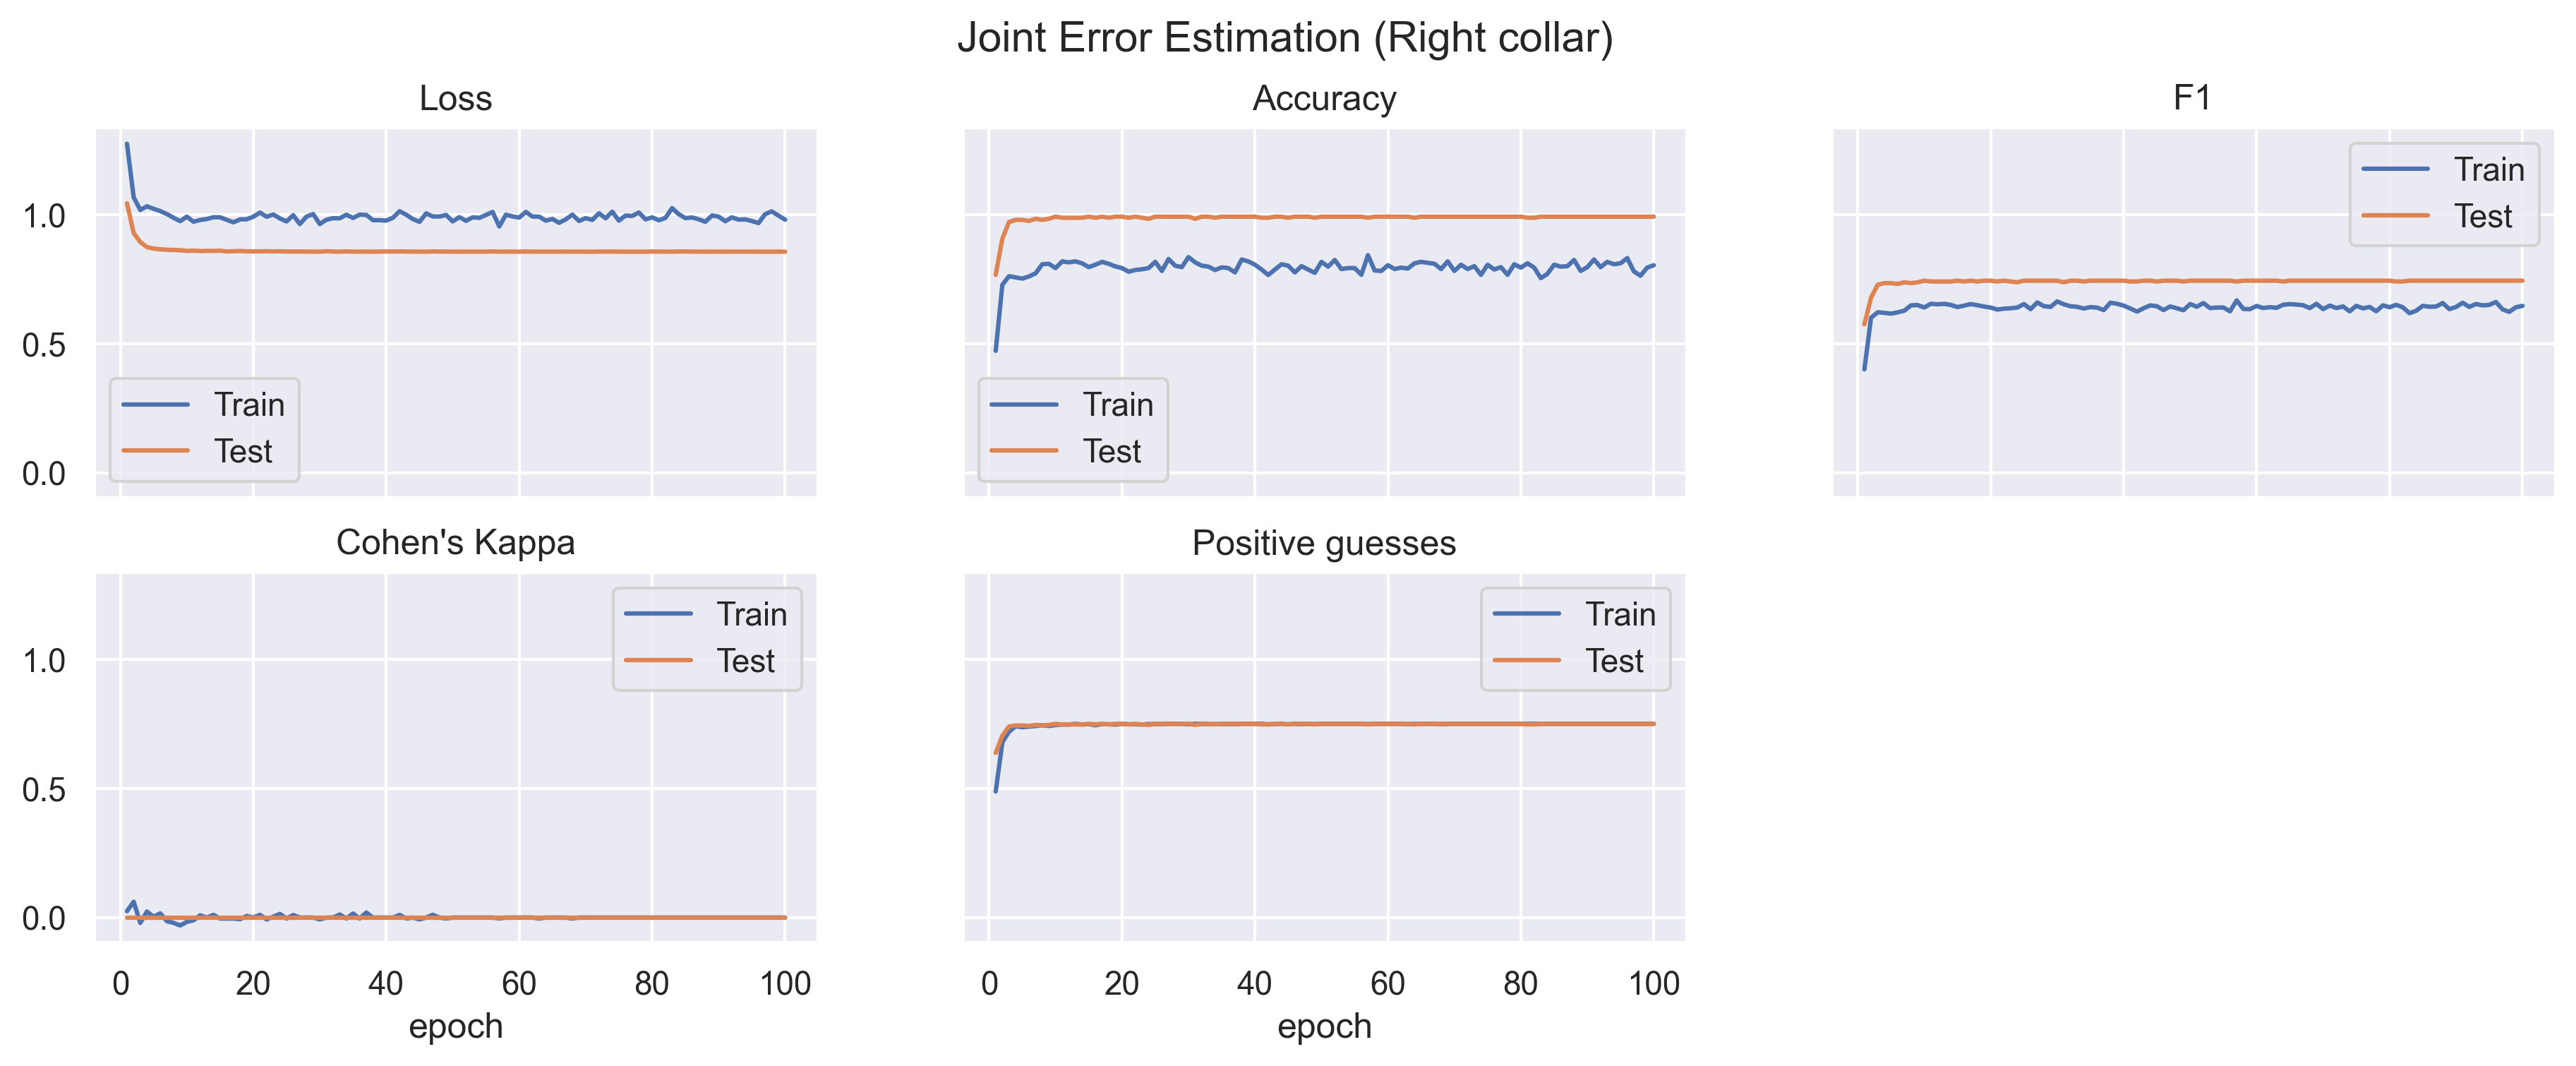
\includegraphics[width=\textwidth]{figures/Results/v1_bs_60_is_64_e_100/jt/Right collar_ErrorEstimation.png}
      \caption{Right Collar Error Estimation}
      \label{fig:v1_rico_jt_ee}
  \end{subfigure}
\end{figure}


\begin{figure}[!ht]
  \centering
  \begin{subfigure}[b]{0.47\linewidth}
      \centering
      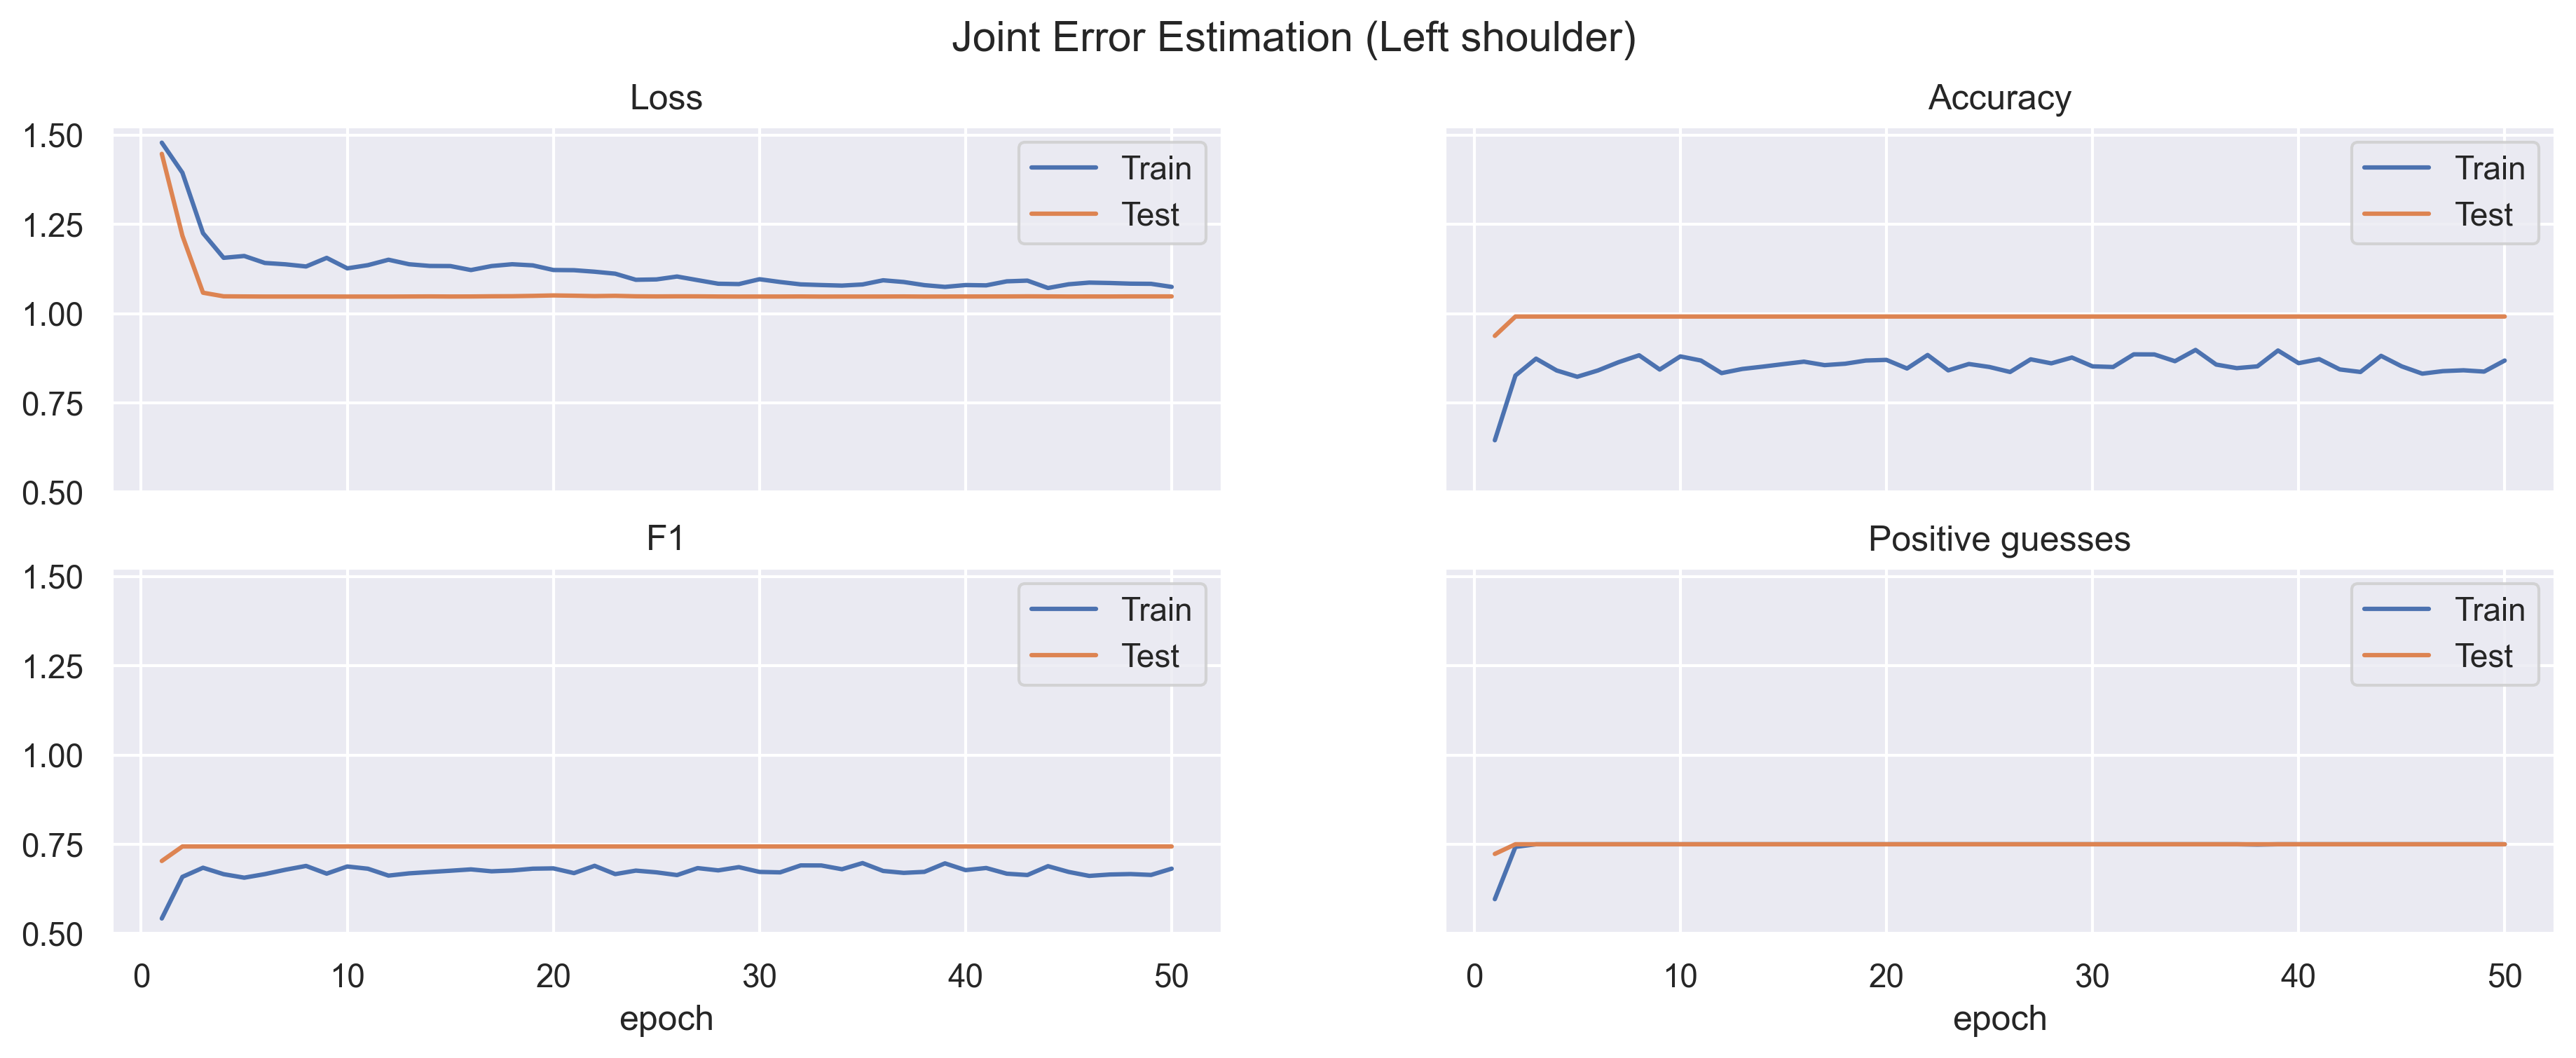
\includegraphics[width=\textwidth]{figures/Results/v1_bs_60_is_64_e_100/jt/Left shoulder_ErrorEstimation.png}
      \caption{Left Shoulder Error Estimation}
      \label{fig:v1_lesh_jt_ee}
  \end{subfigure}
  \hfill
  \begin{subfigure}[b]{0.47\linewidth}
      \centering
      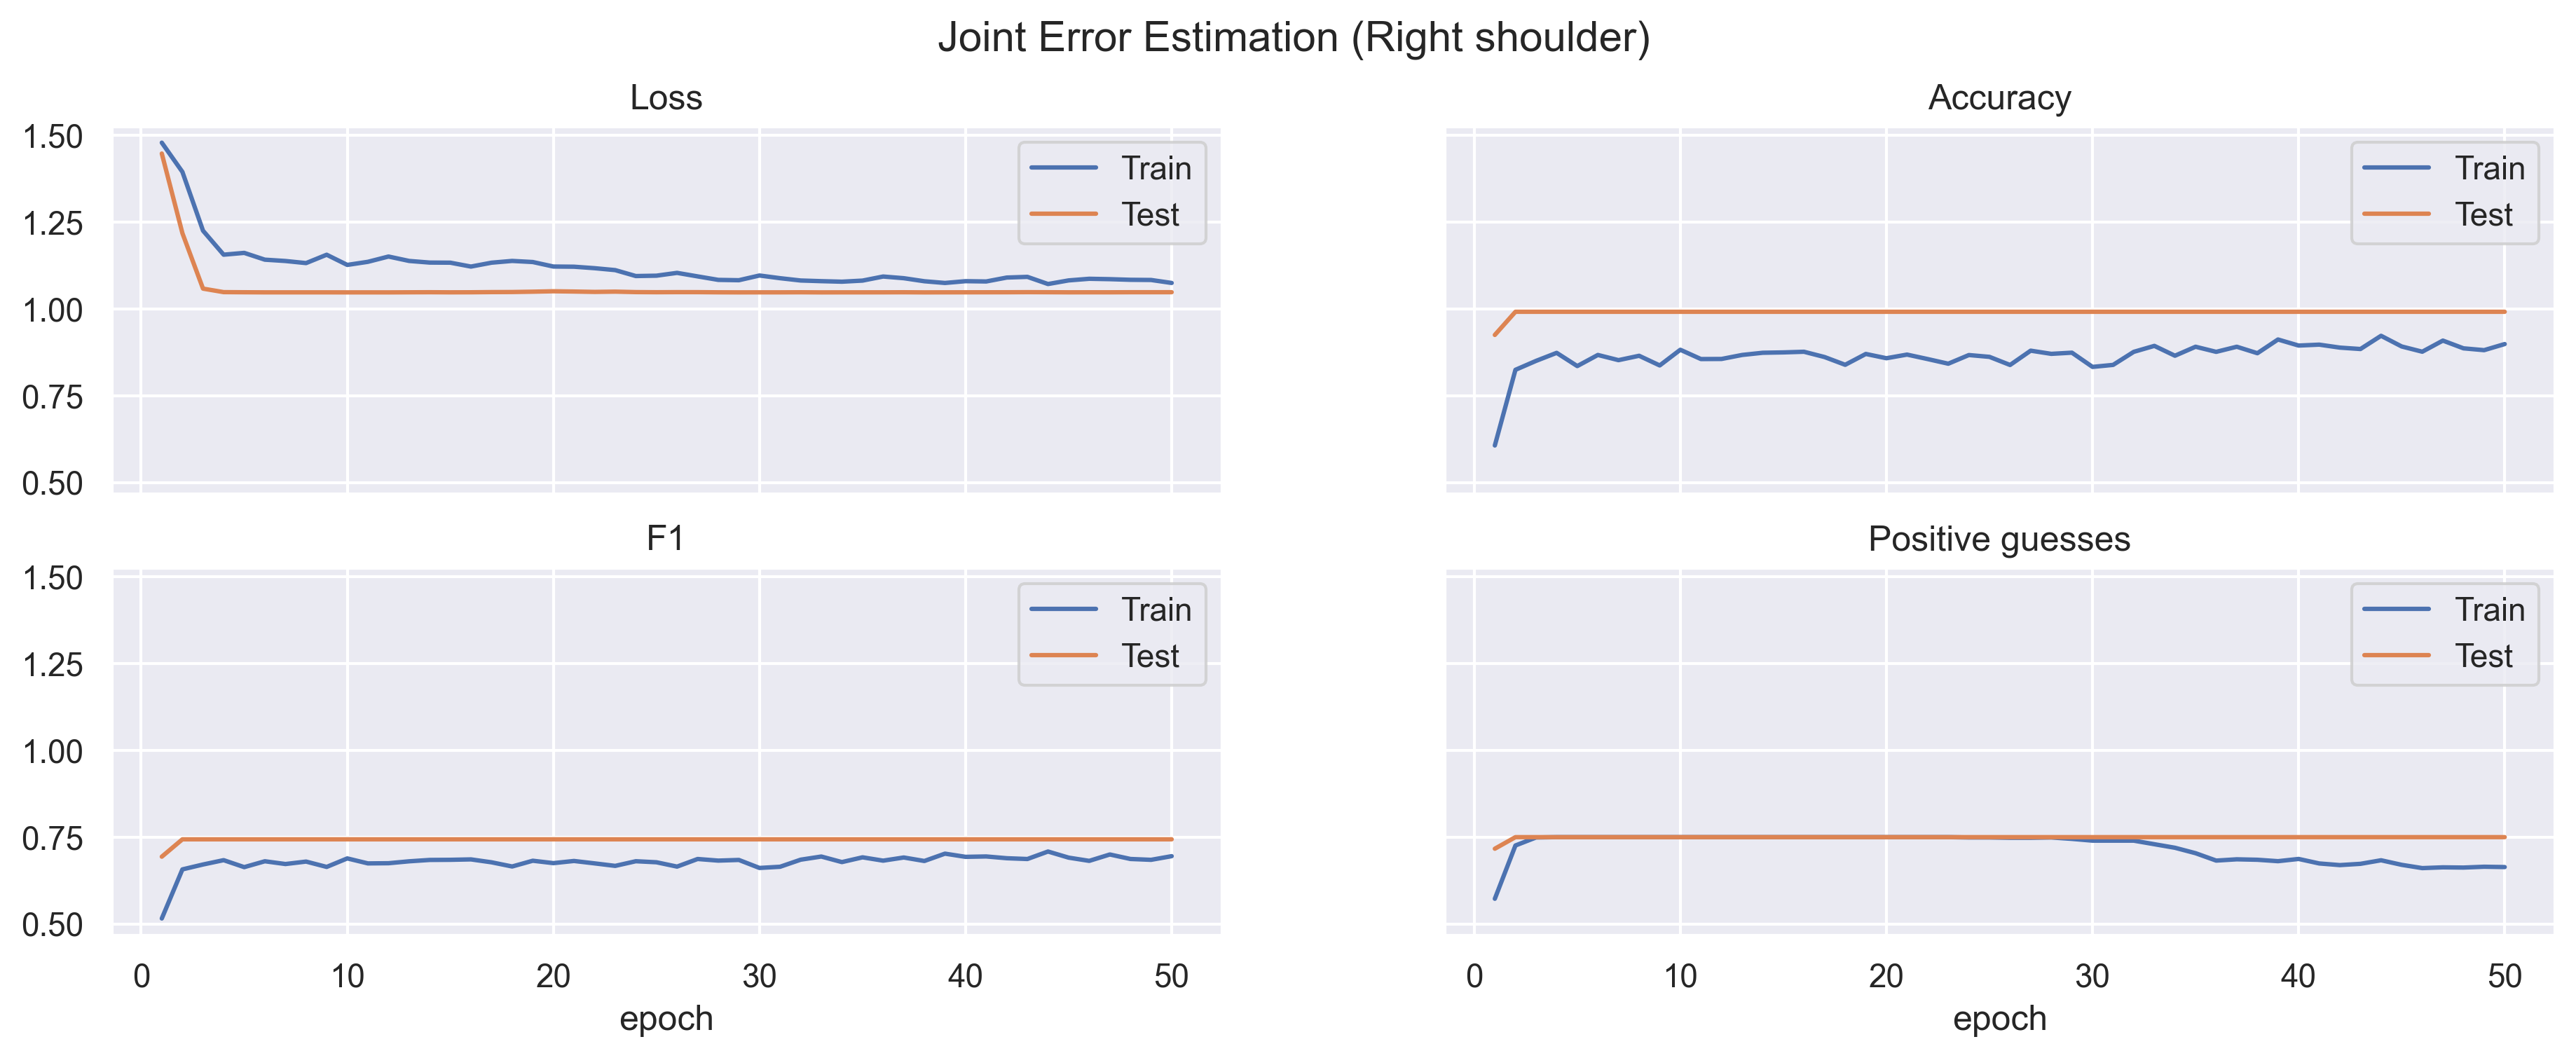
\includegraphics[width=\textwidth]{figures/Results/v1_bs_60_is_64_e_100/jt/Right shoulder_ErrorEstimation.png}
      \caption{Right Shoulder Error Estimation}
      \label{fig:v1_rish_jt_ee}
  \end{subfigure}
  \hfill
  \begin{subfigure}[b]{0.47\linewidth}
      \centering
      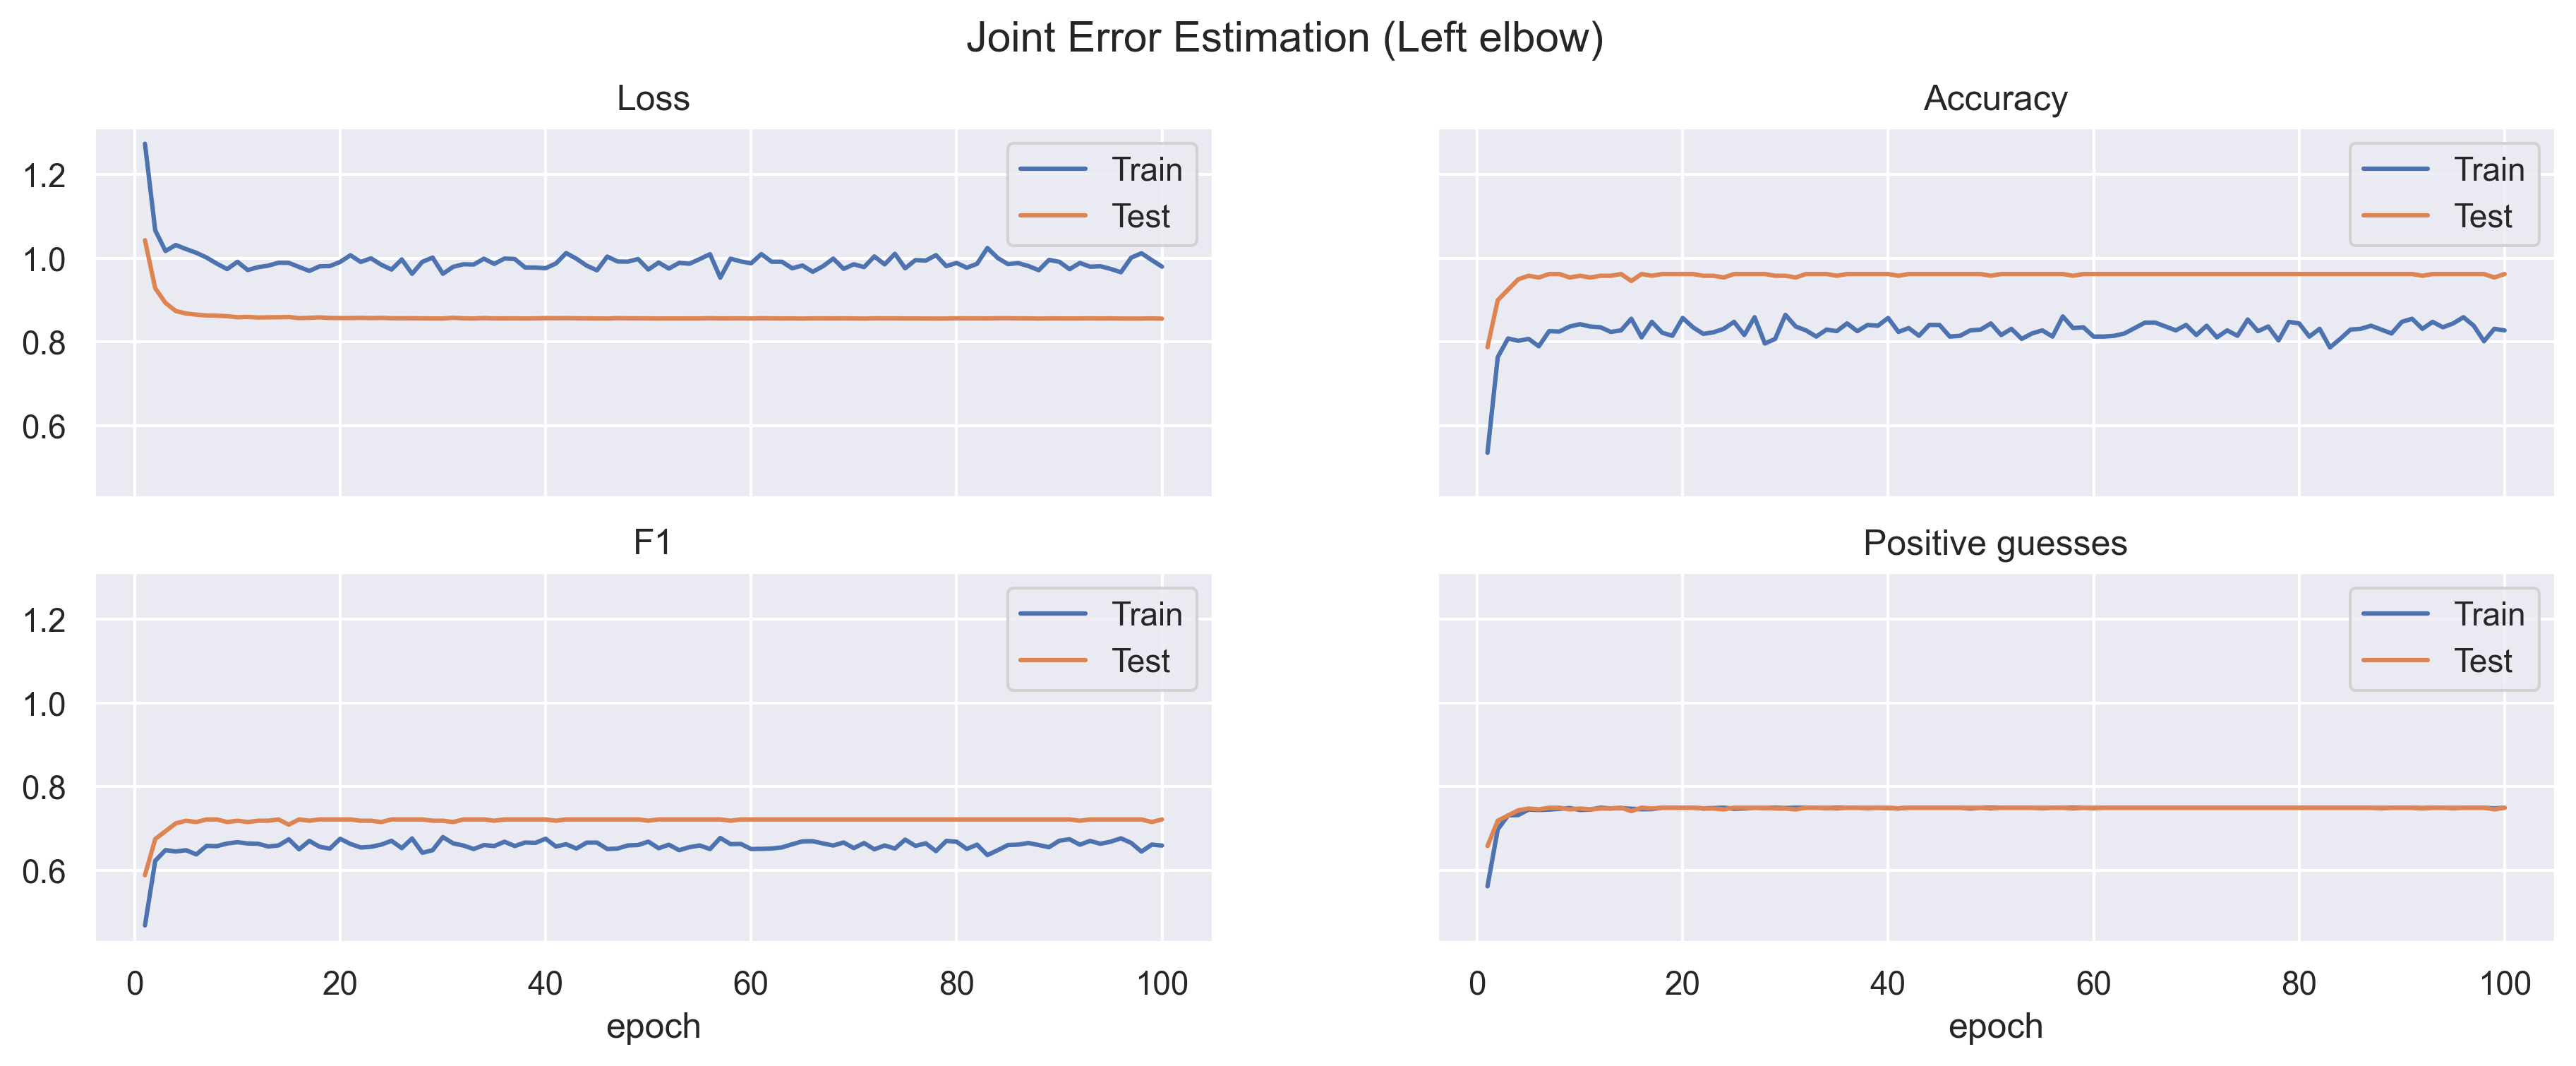
\includegraphics[width=\textwidth]{figures/Results/v1_bs_60_is_64_e_100/jt/Left elbow_ErrorEstimation.png}
      \caption{Left Elbow Error Estimation}
      \label{fig:v1_leel_jt_ee}
  \end{subfigure}
  \hfill
  \begin{subfigure}[b]{0.47\linewidth}
      \centering
      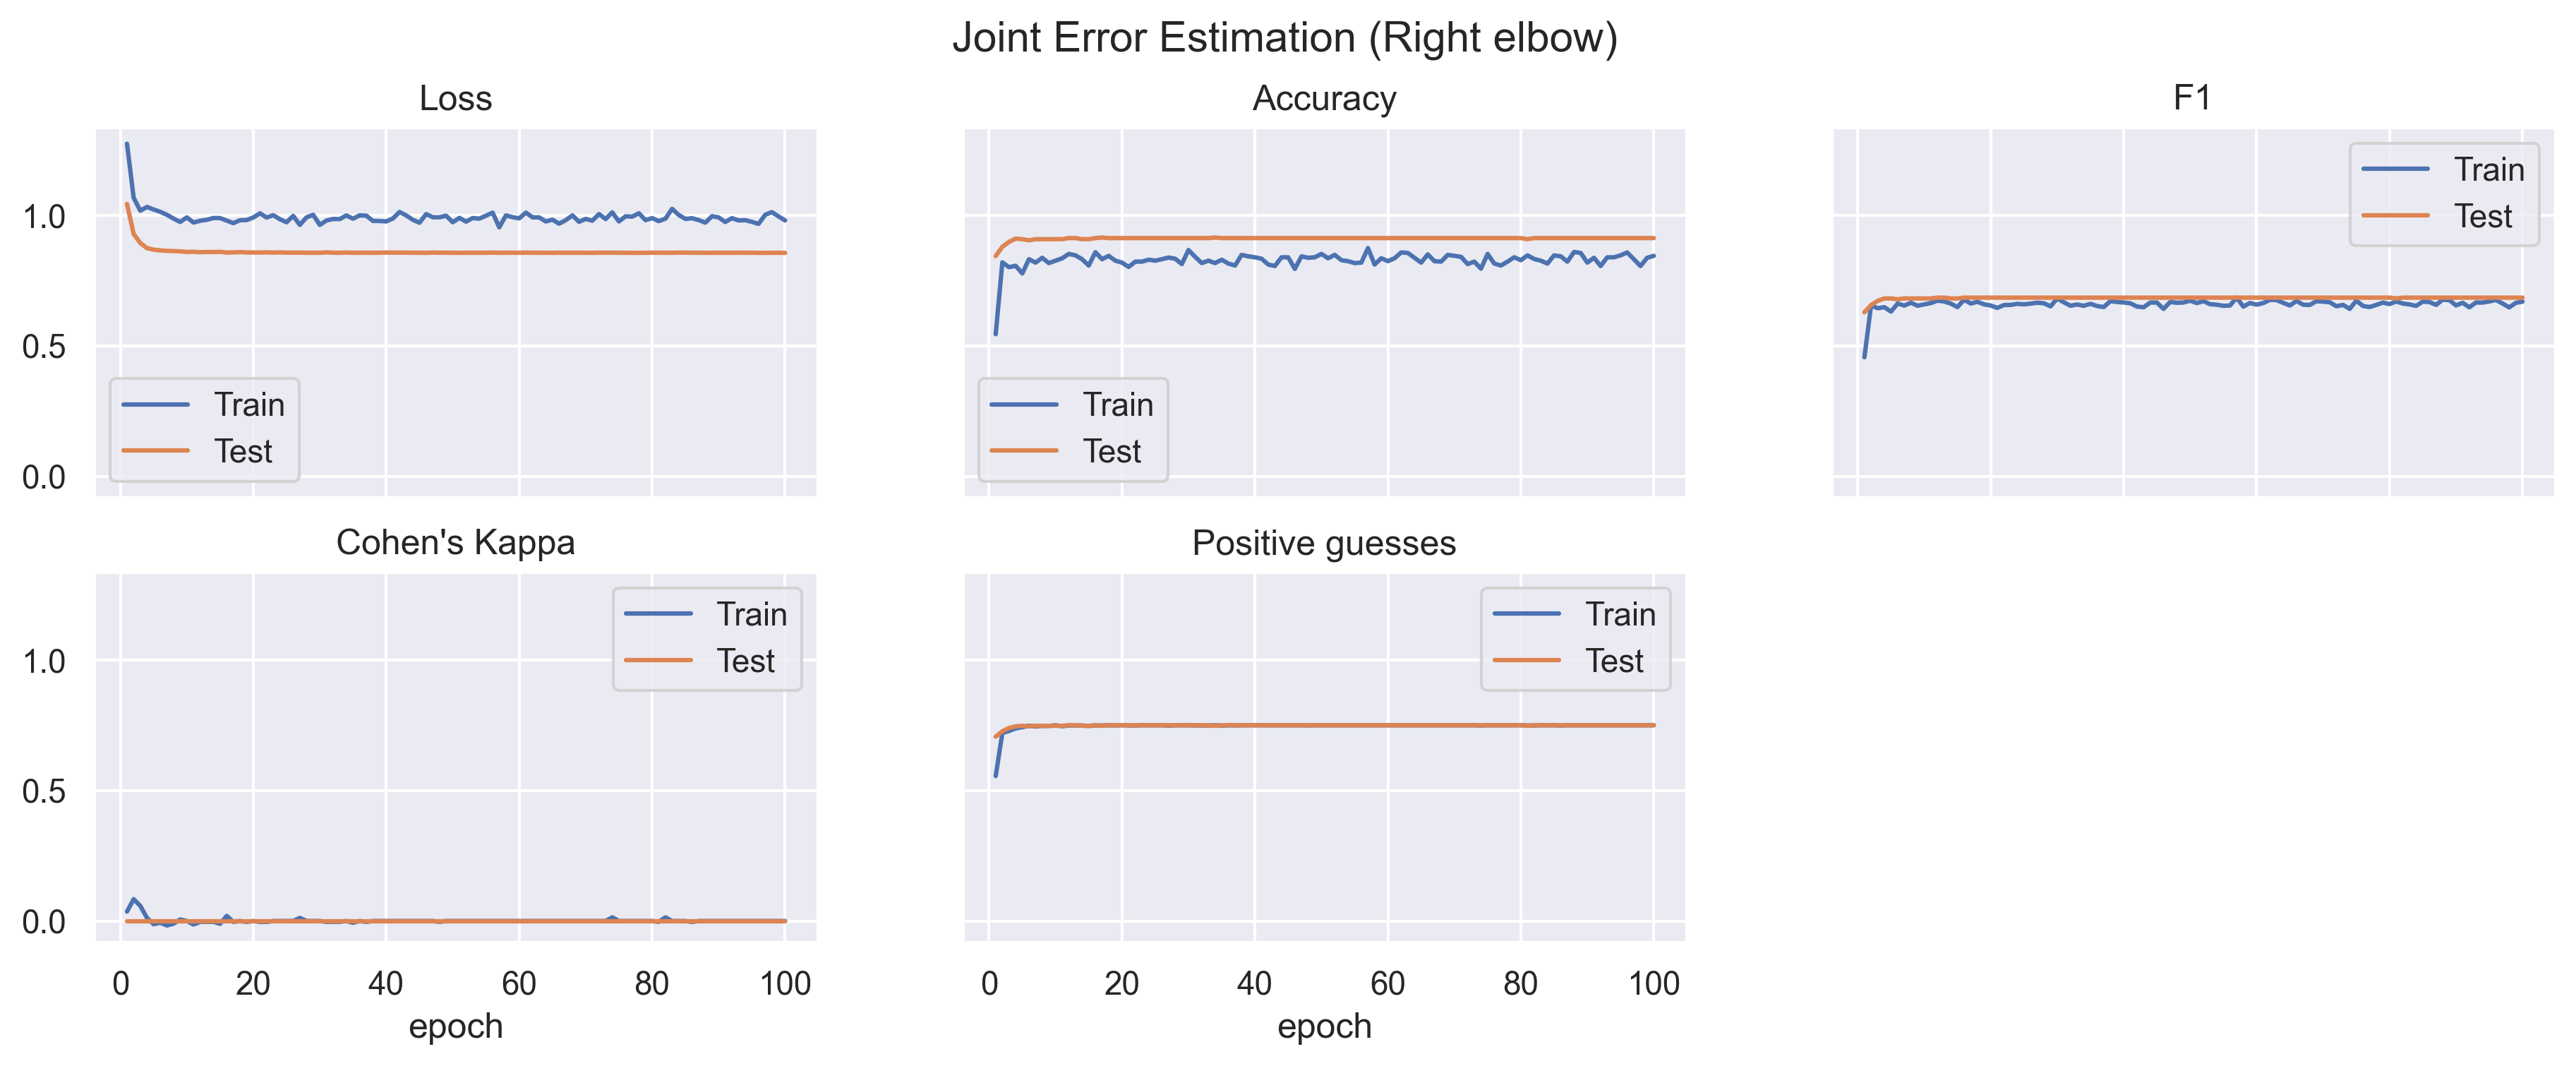
\includegraphics[width=\textwidth]{figures/Results/v1_bs_60_is_64_e_100/jt/Right elbow_ErrorEstimation.png}
      \caption{Right Elbow Error Estimation}
      \label{fig:v1_reel_jt_ee}
  \end{subfigure}
\end{figure}


\begin{figure}[!ht]
  \centering
  \begin{subfigure}[b]{0.47\linewidth}
      \centering
      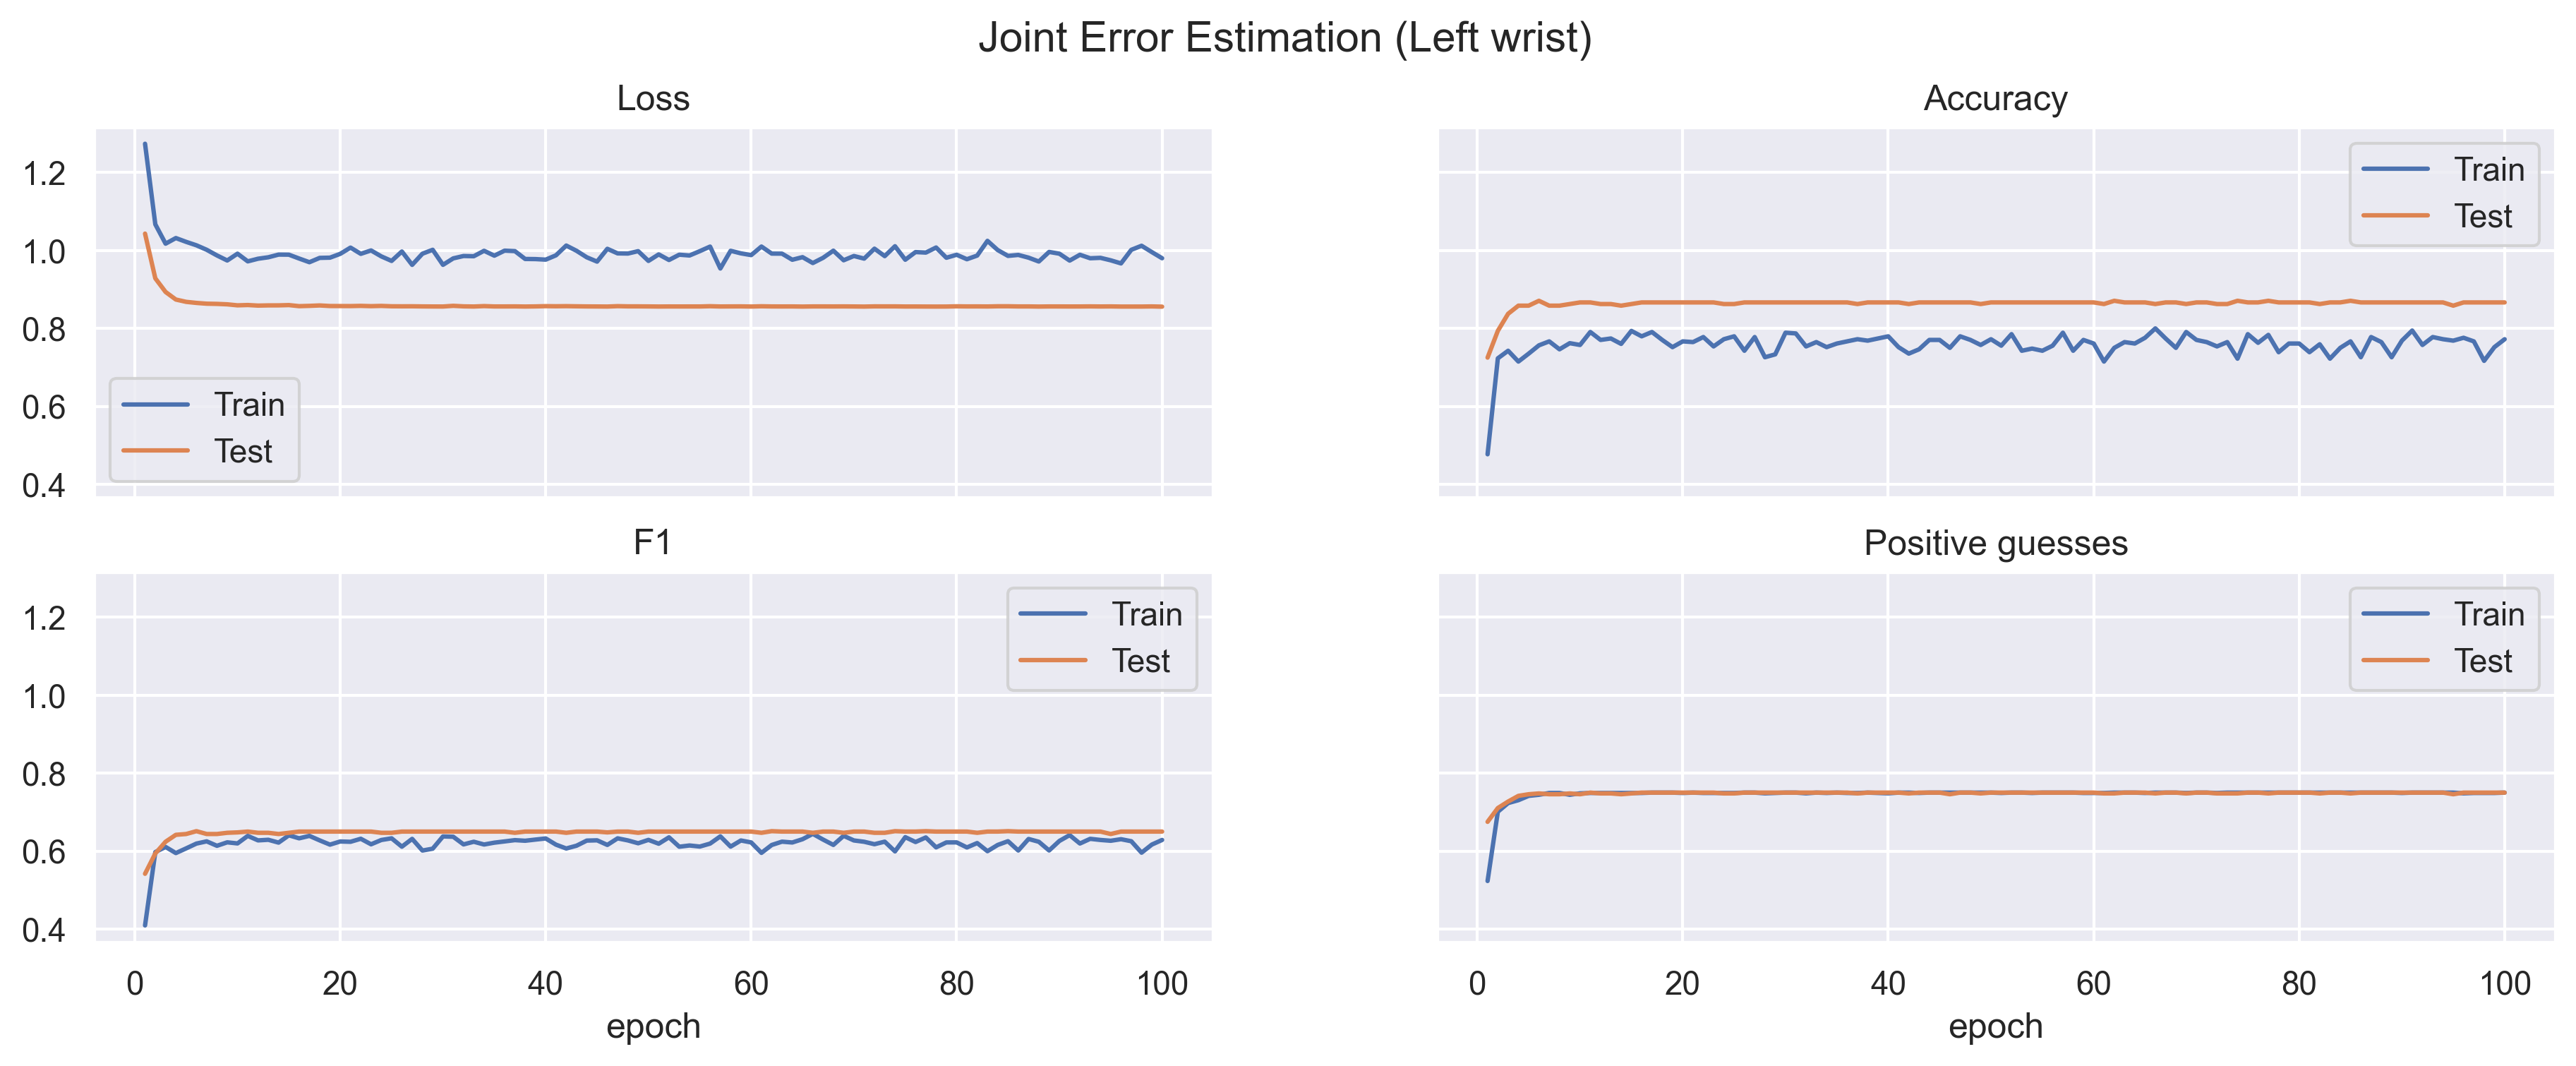
\includegraphics[width=\textwidth]{figures/Results/v1_bs_60_is_64_e_100/jt/Left wrist_ErrorEstimation.png}
      \caption{Left Wrist Error Estimation}
      \label{fig:v1_lewr_jt_ee}
  \end{subfigure}
  \hfill
  \begin{subfigure}[b]{0.47\linewidth}
      \centering
      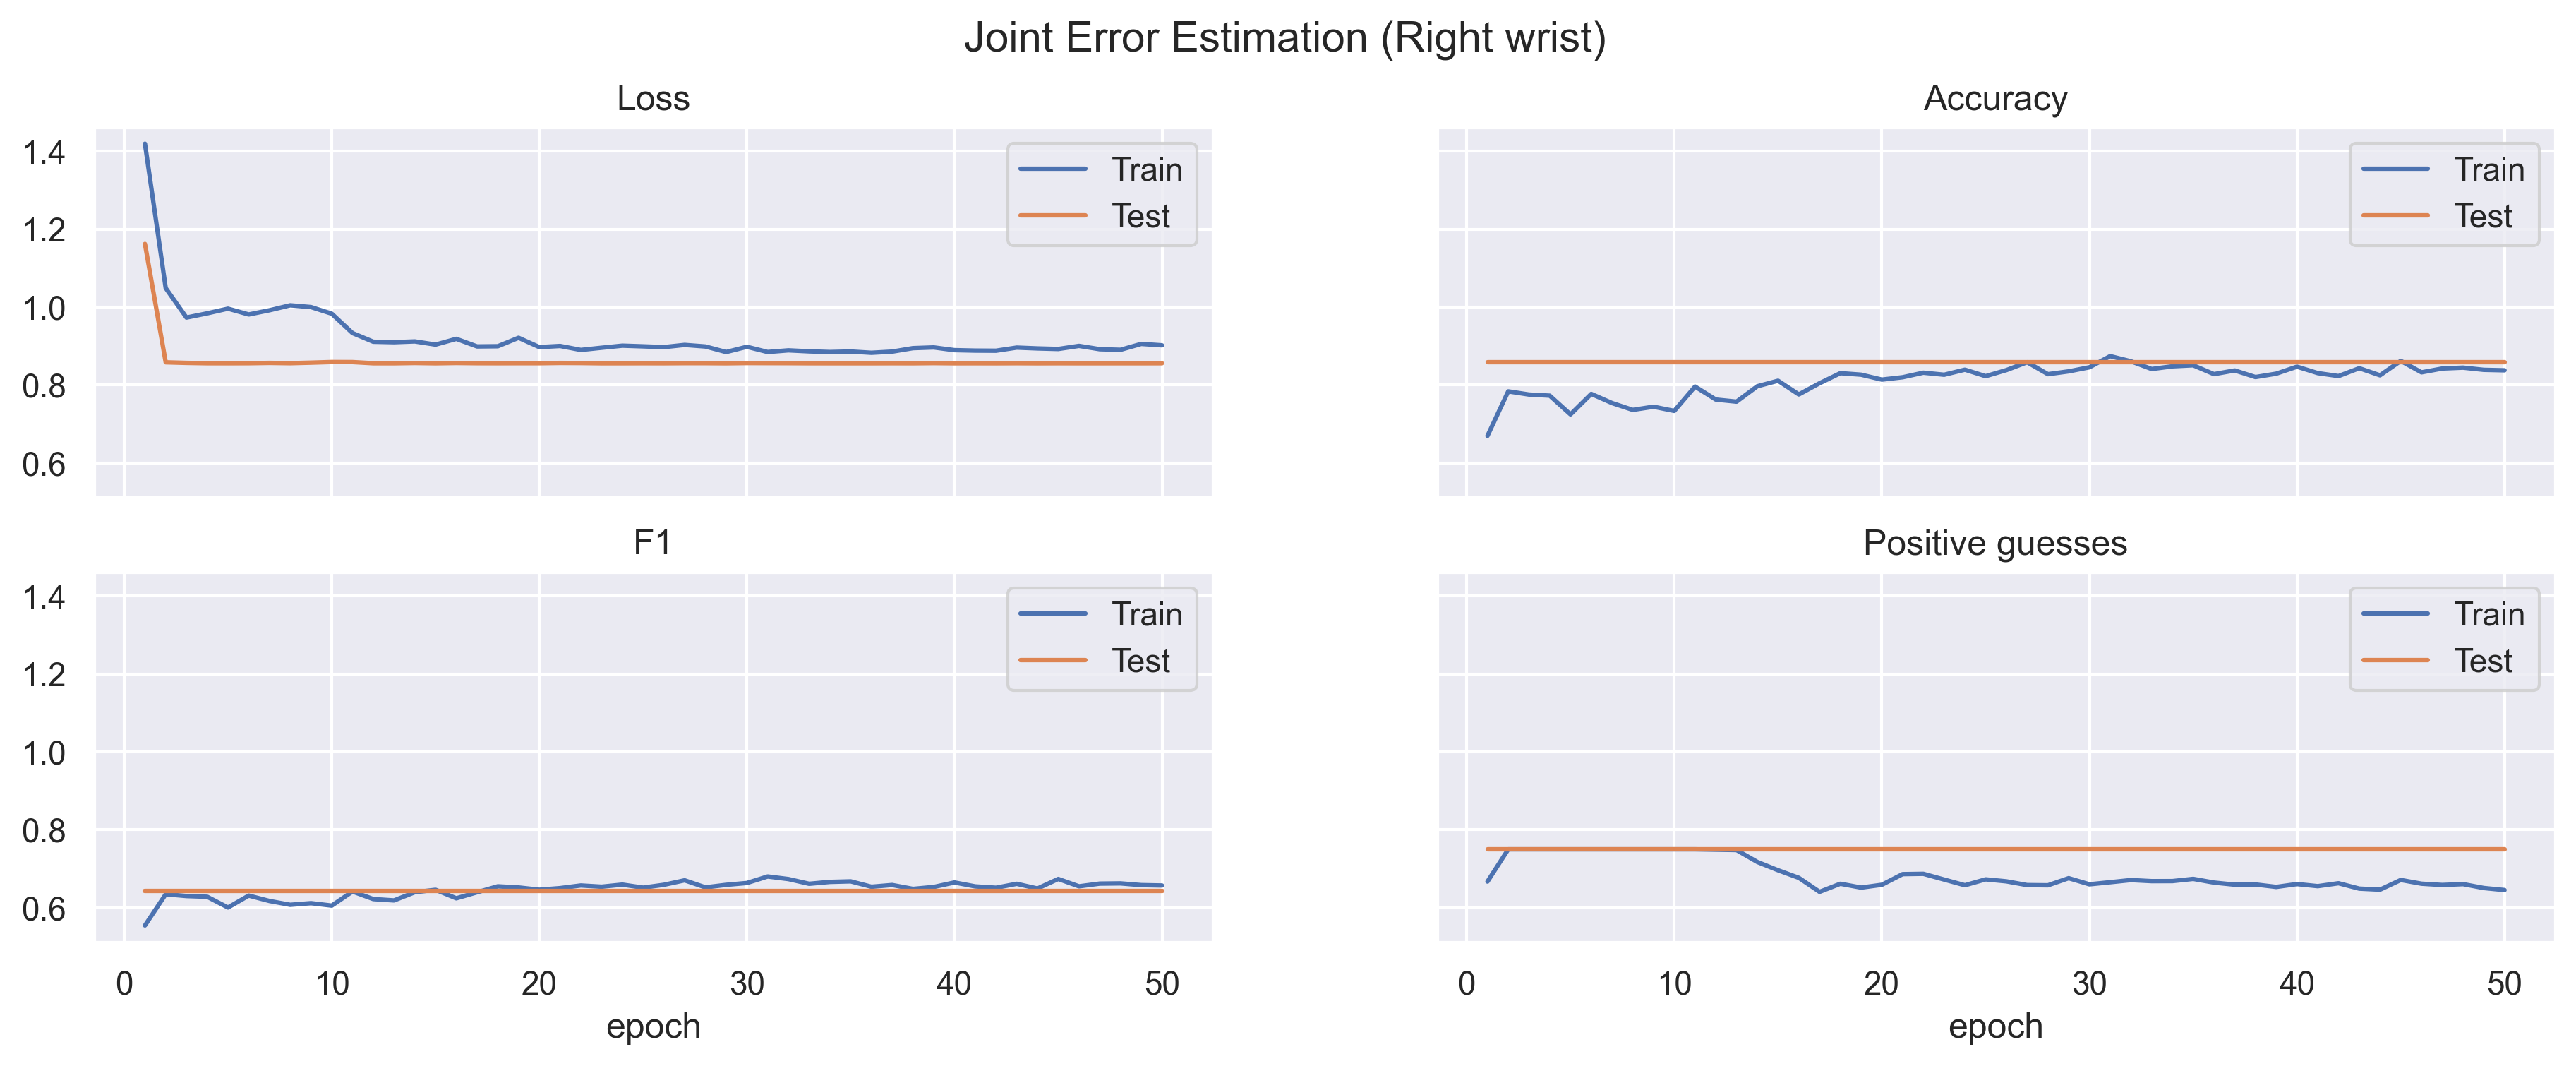
\includegraphics[width=\textwidth]{figures/Results/v1_bs_60_is_64_e_100/jt/Right wrist_ErrorEstimation.png}
      \caption{Right Wrist Error Estimation}
      \label{fig:v1_riwr_jt_ee}
  \end{subfigure}
  \hfill
  \begin{subfigure}[b]{0.47\linewidth}
      \centering
      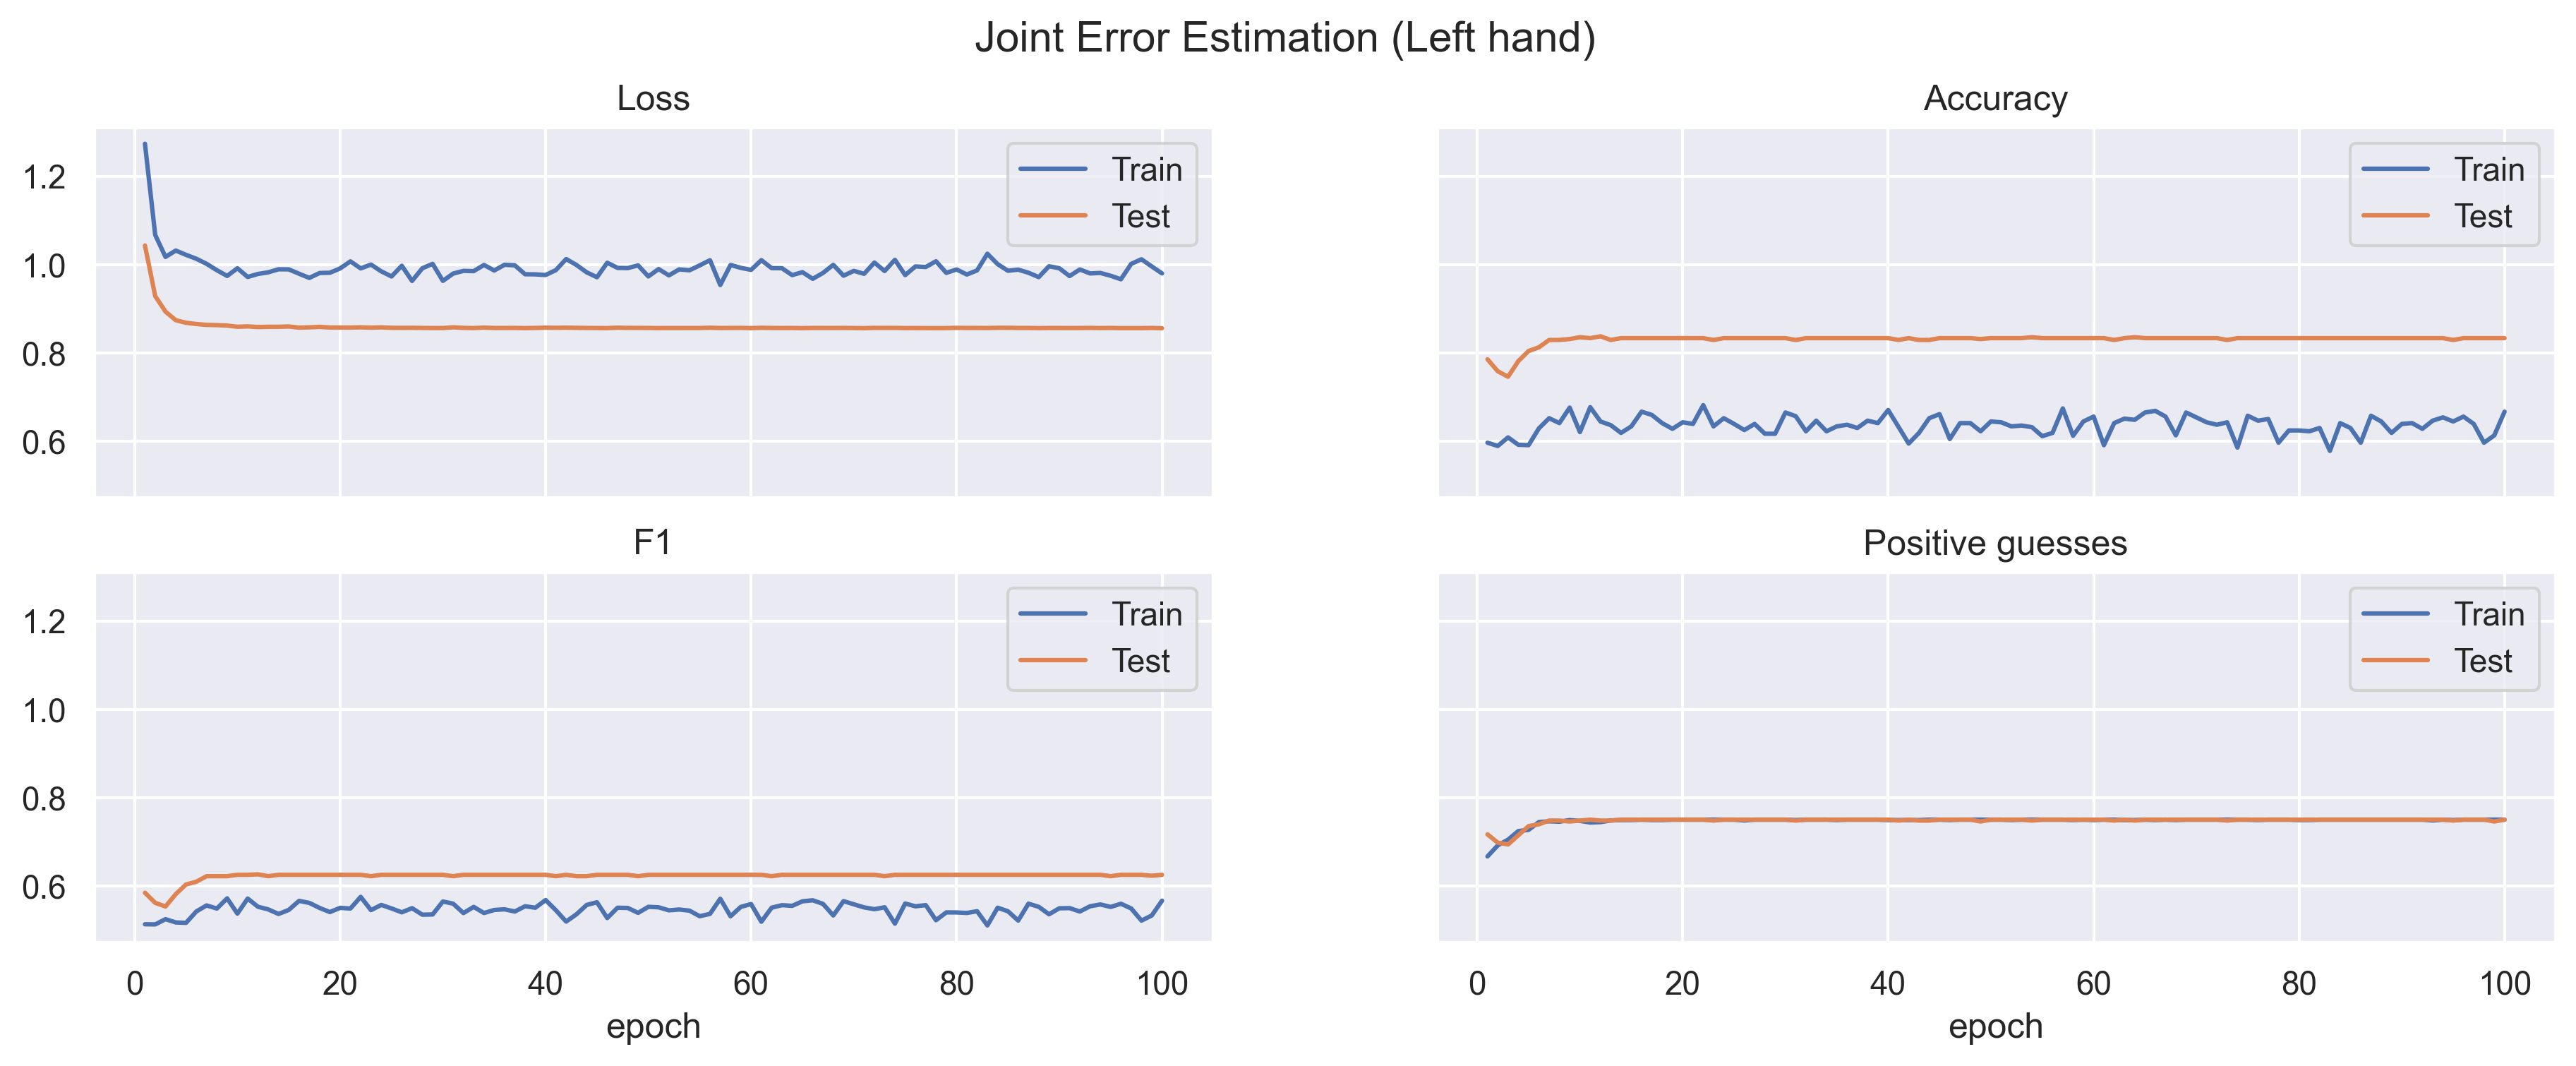
\includegraphics[width=\textwidth]{figures/Results/v1_bs_60_is_64_e_100/jt/Left hand_ErrorEstimation.png}
      \caption{Left Hand Error Estimation}
      \label{fig:v1_leha_jt_ee}
  \end{subfigure}
  \hfill
  \begin{subfigure}[b]{0.47\linewidth}
      \centering
      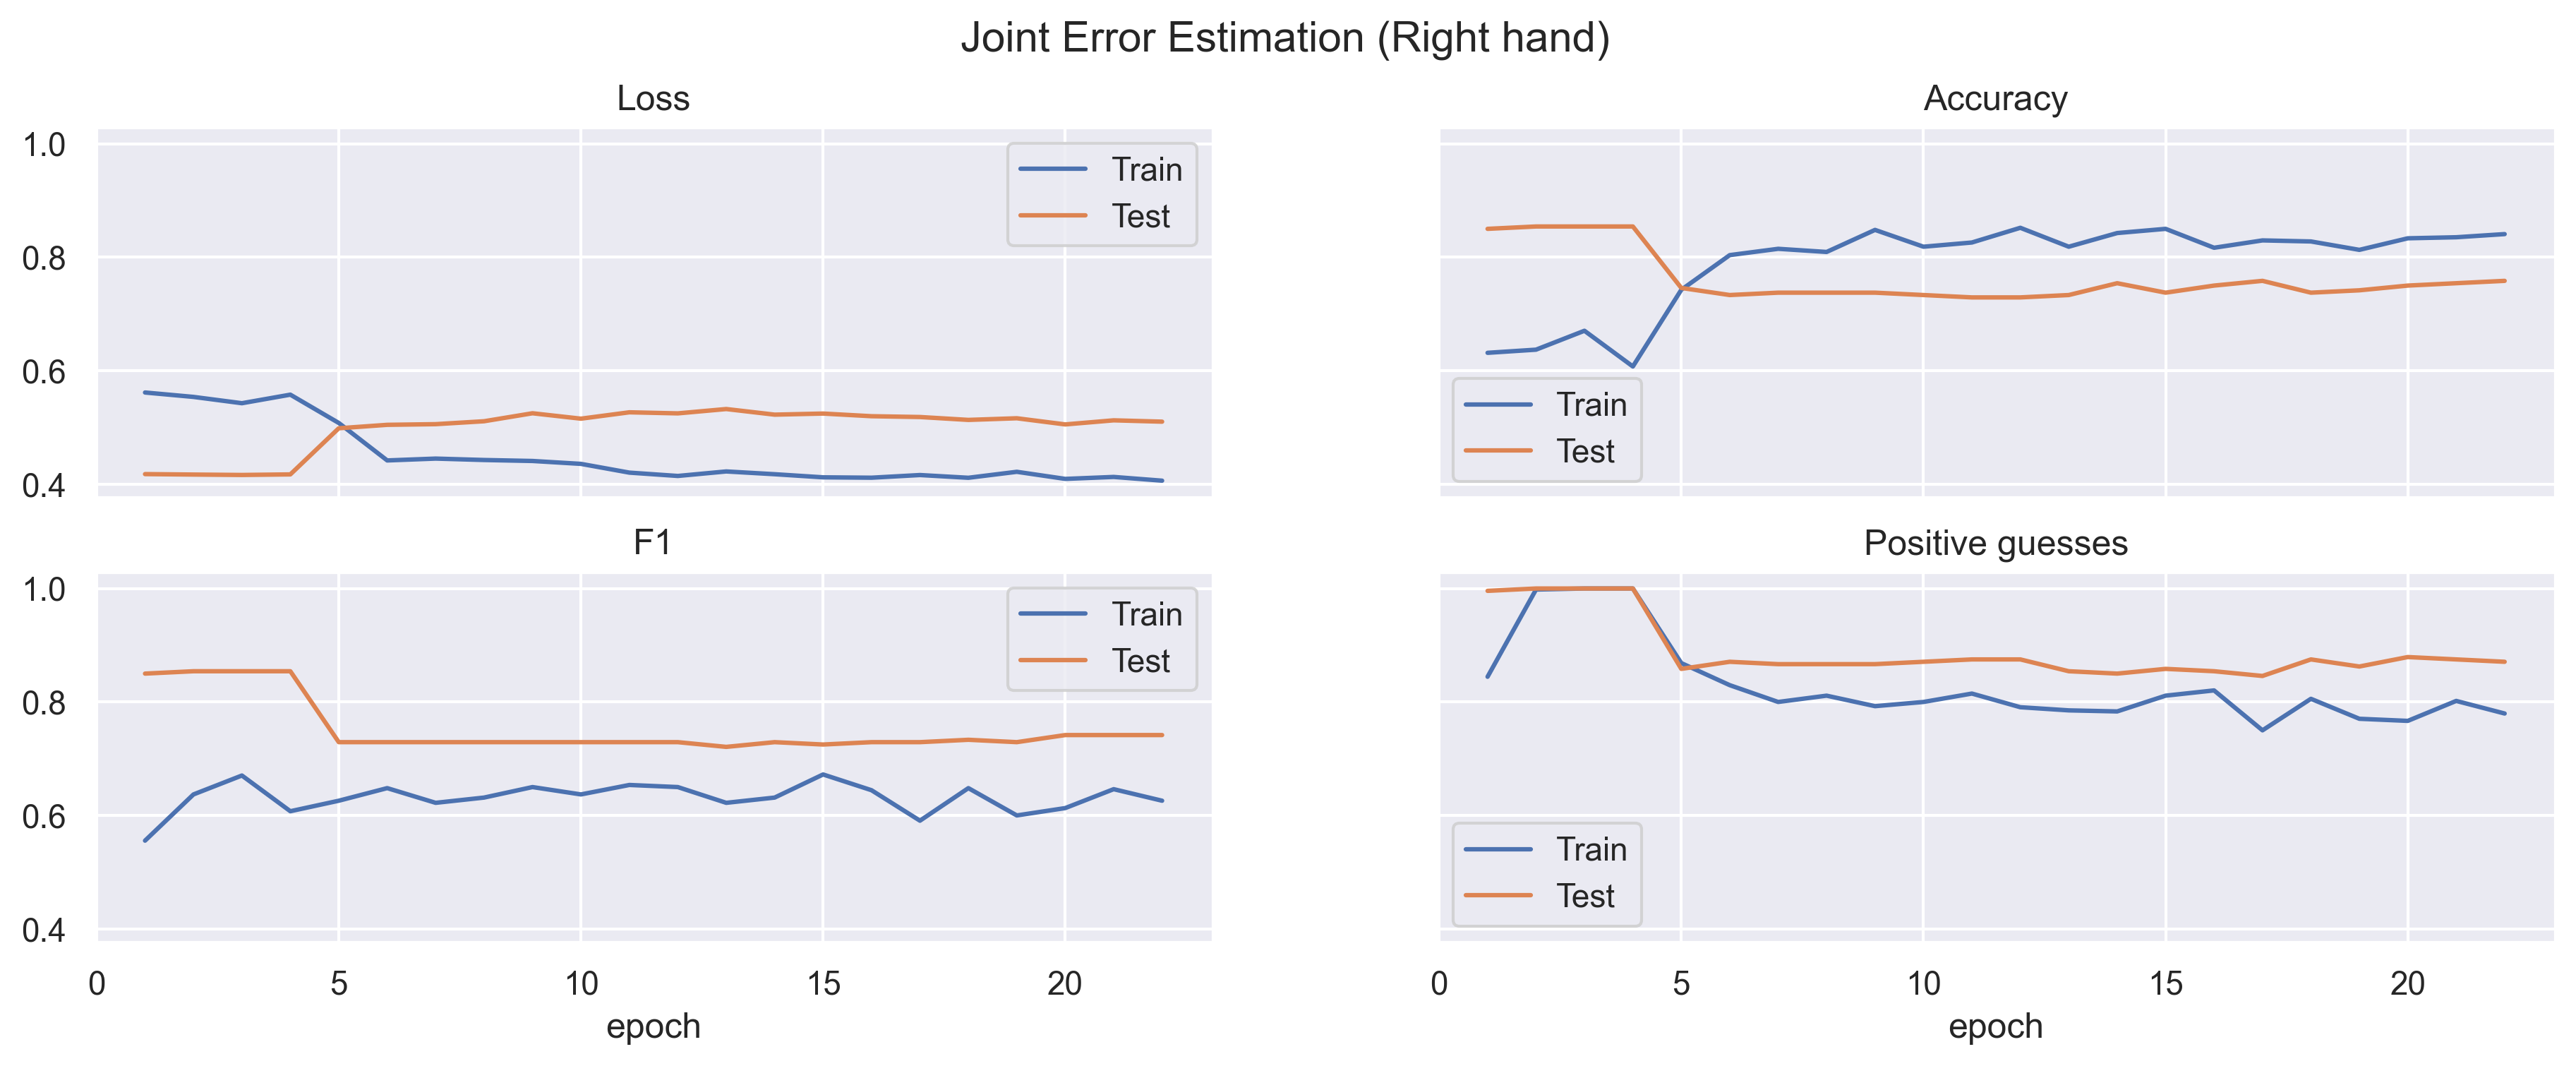
\includegraphics[width=\textwidth]{figures/Results/v1_bs_60_is_64_e_100/jt/Right hand_ErrorEstimation.png}
      \caption{Left Arm Error Estimation}
      \label{fig:v1_riha_jt_ee}
  \end{subfigure}
\end{figure}

\begin{figure}[!ht]
  \centering
  \begin{subfigure}[b]{0.47\linewidth}
      \centering
      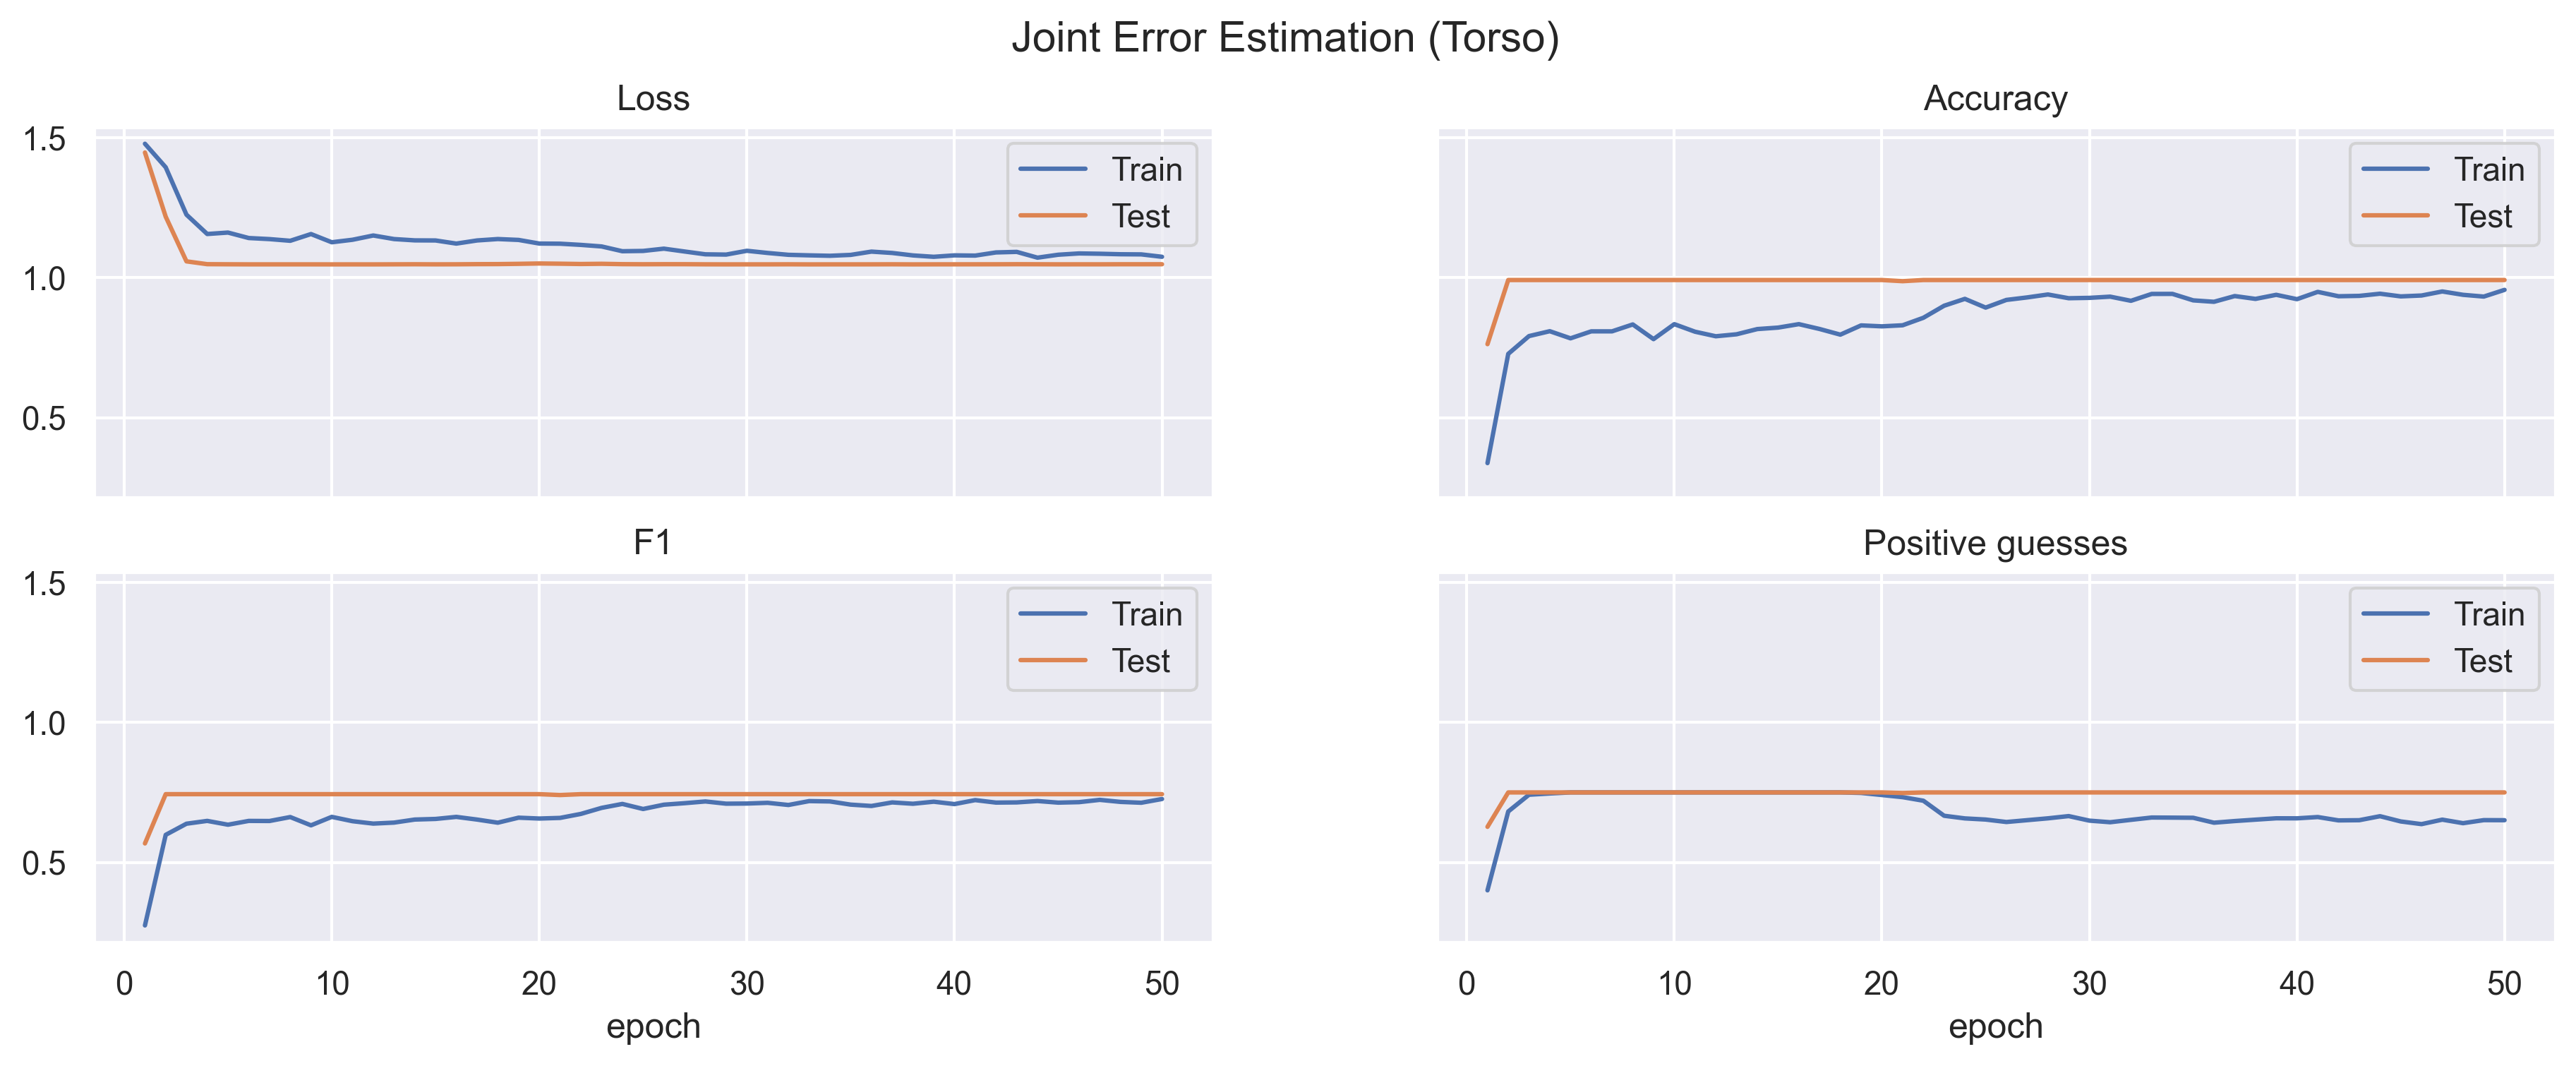
\includegraphics[width=\textwidth]{figures/Results/v1_bs_60_is_64_e_100/jt/Torso_ErrorEstimation.png}
      \caption{Torso Error Estimation}
      \label{fig:v1_torso_jt_ee}
  \end{subfigure}
  \hfill
  \begin{subfigure}[b]{0.47\linewidth}
    \centering
    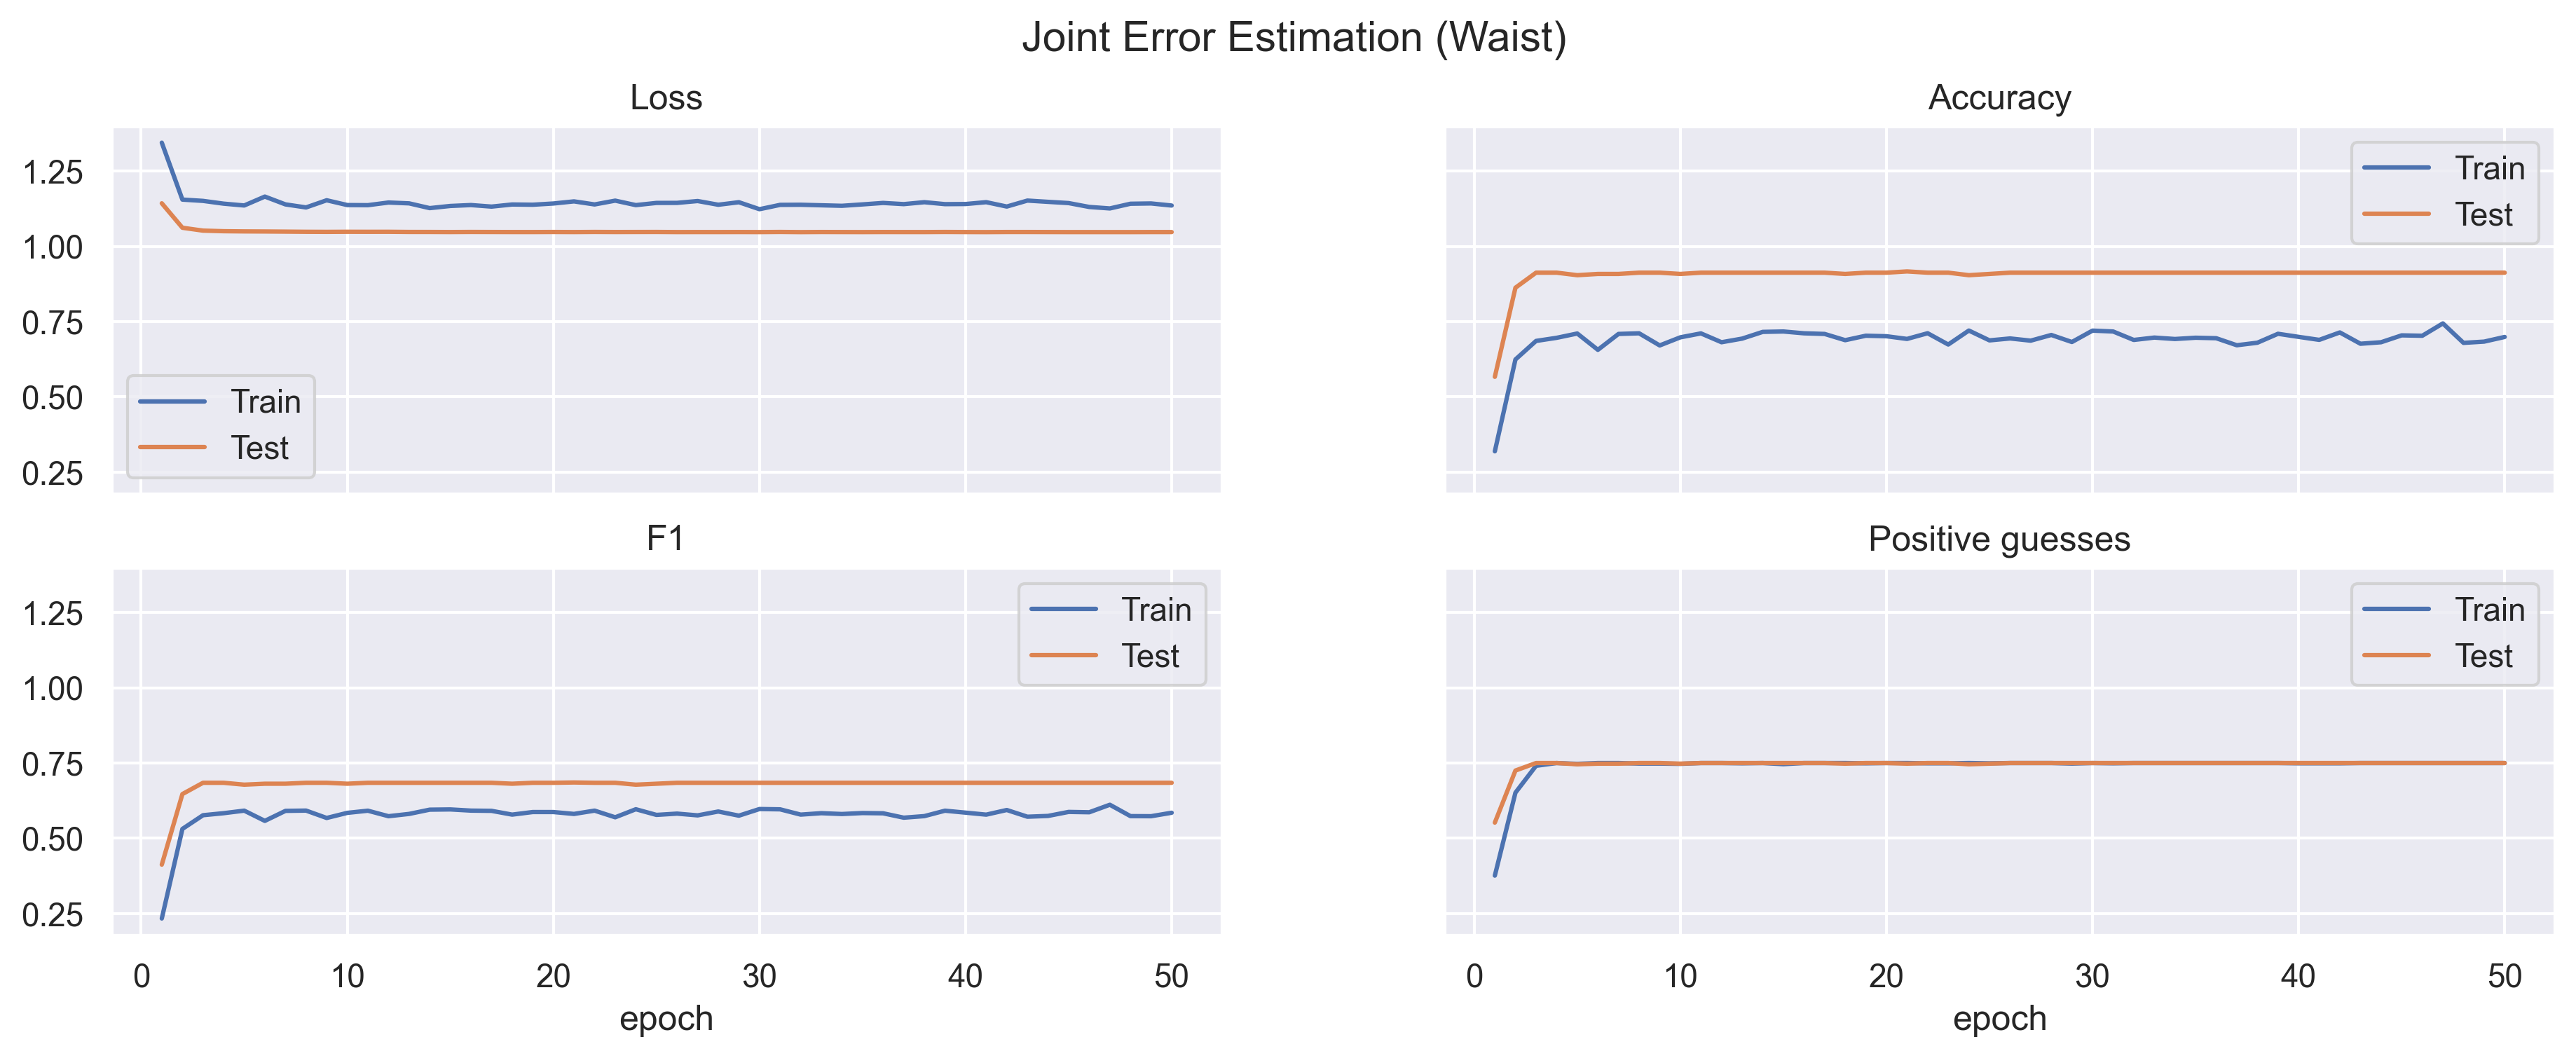
\includegraphics[width=\textwidth]{figures/Results/v1_bs_60_is_64_e_100/jt/Waist_ErrorEstimation.png}
    \caption{Waist Error Estimation}
    \label{fig:v1_waist_jt_ee}
  \end{subfigure}
  \hfill
  \begin{subfigure}[b]{0.47\linewidth}
      \centering
      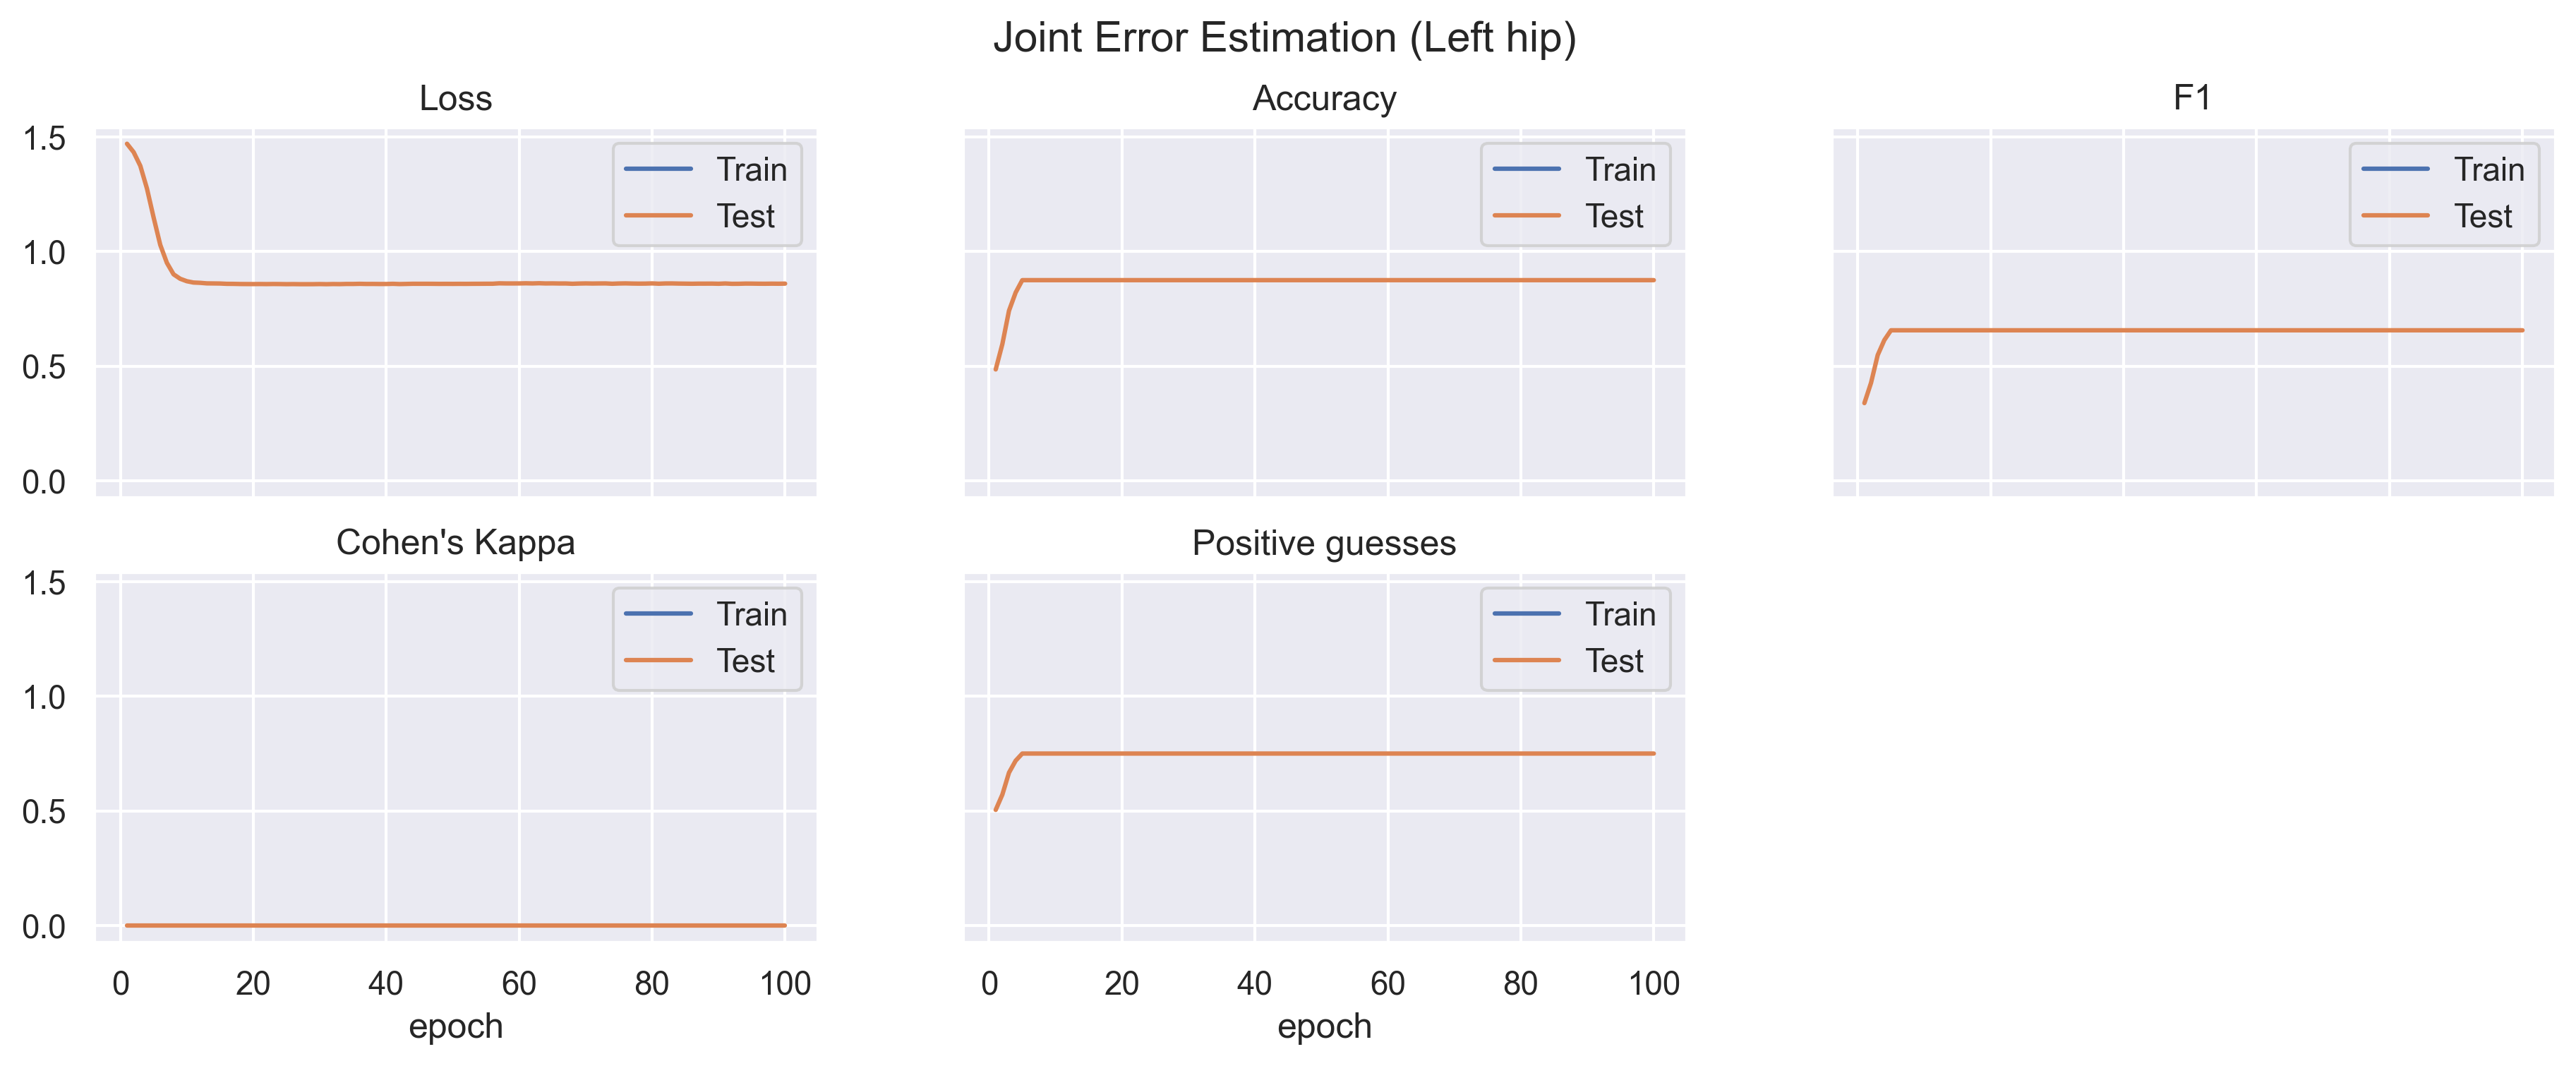
\includegraphics[width=\textwidth]{figures/Results/v1_bs_60_is_64_e_100/jt/Left hip_ErrorEstimation.png}
      \caption{Left Hip Error Estimation}
      \label{fig:v1_lehi_jt_ee}
  \end{subfigure}
  \hfill
  \begin{subfigure}[b]{0.47\linewidth}
      \centering
      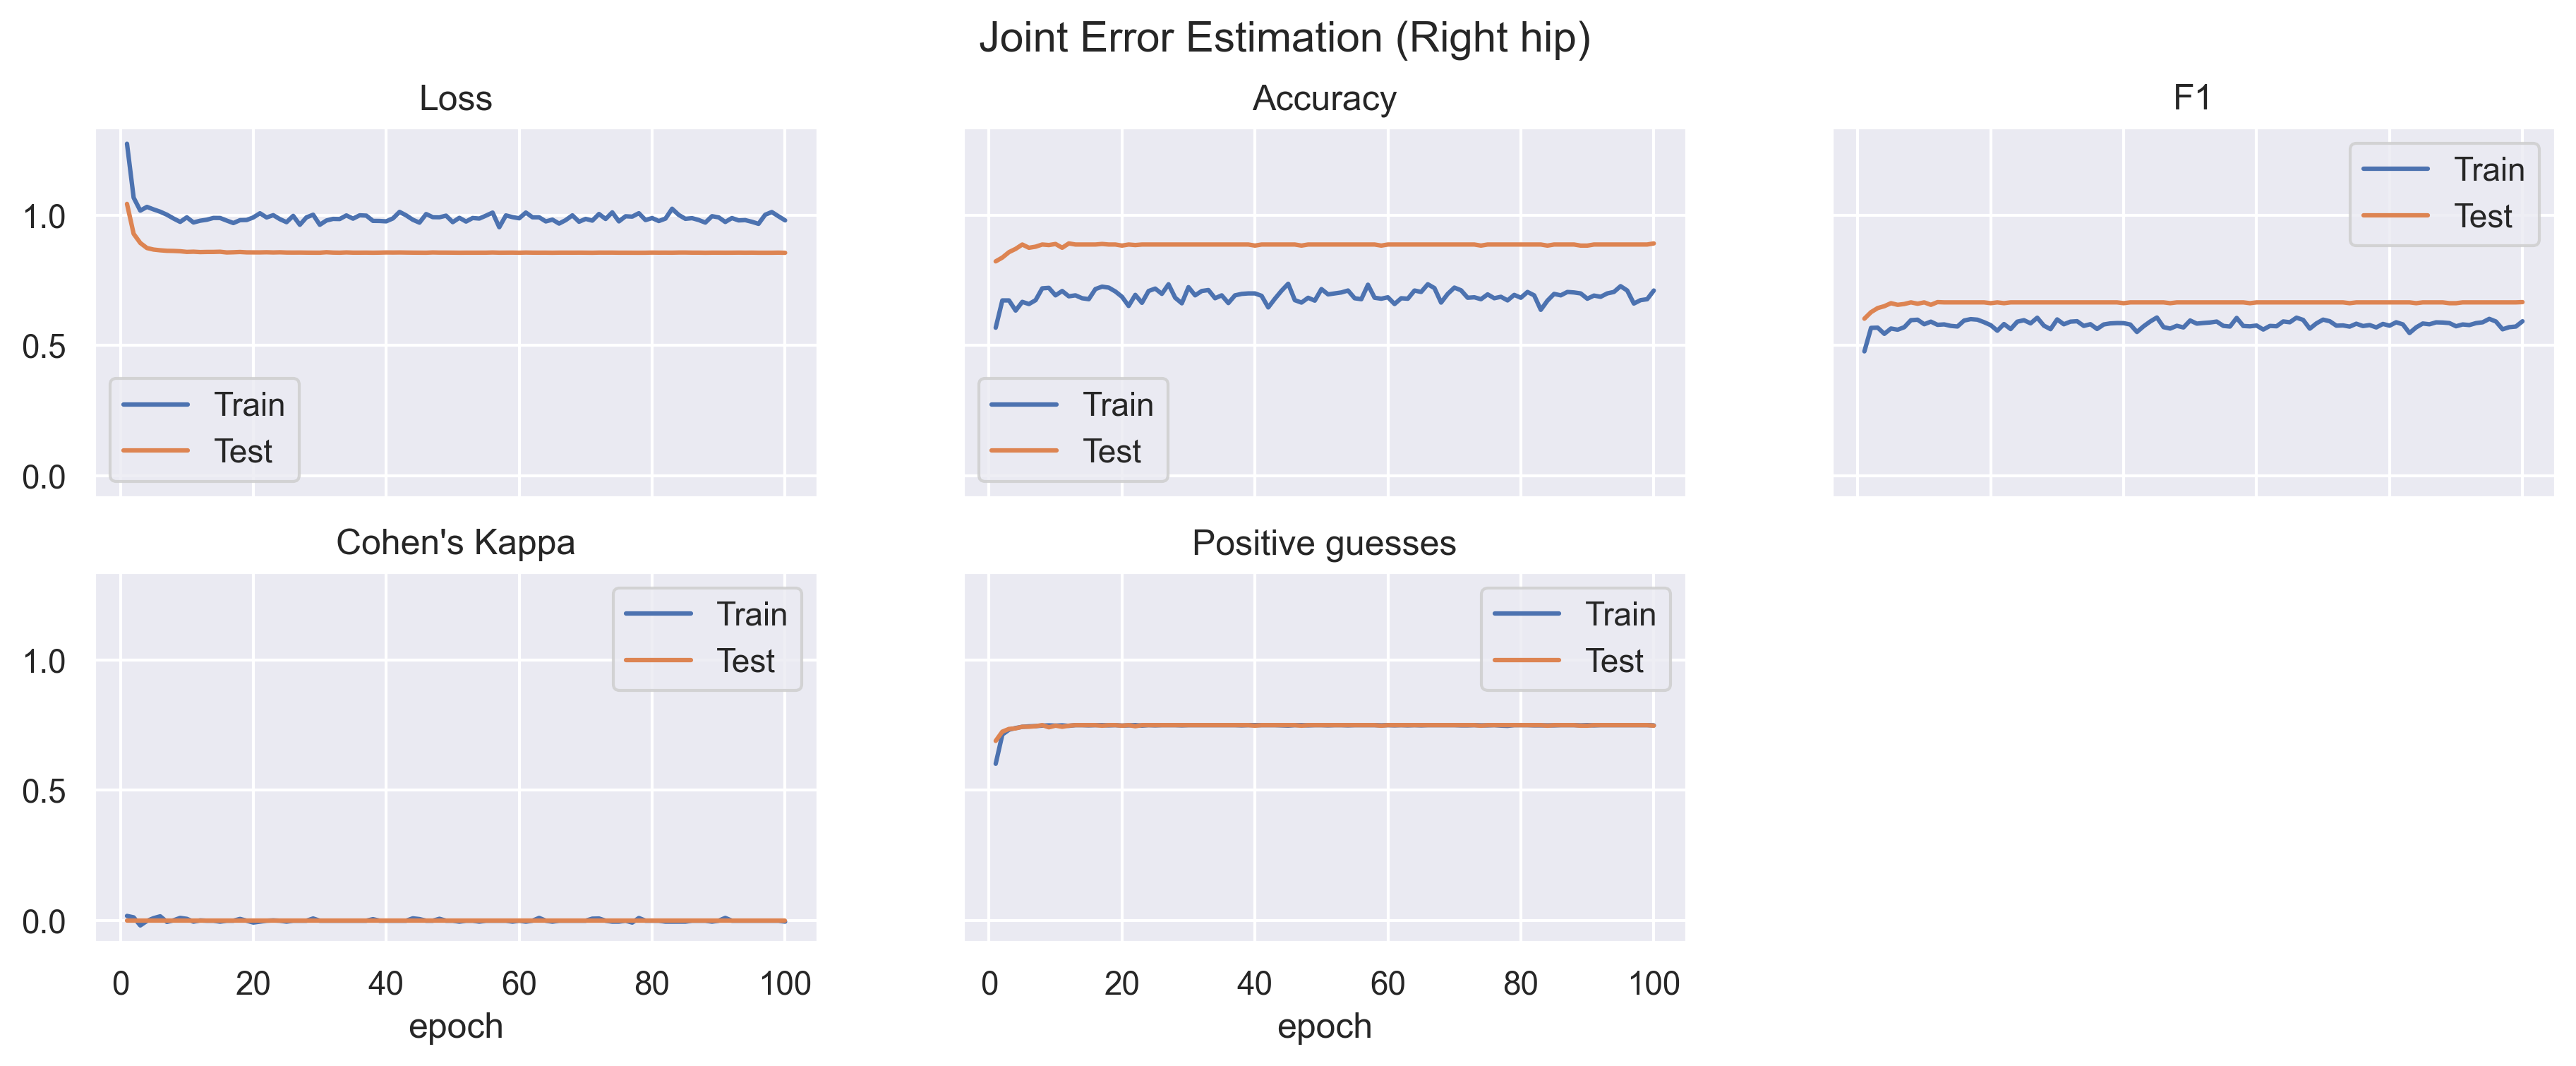
\includegraphics[width=\textwidth]{figures/Results/v1_bs_60_is_64_e_100/jt/Right hip_ErrorEstimation.png}
      \caption{Right hip Error Estimation}
      \label{fig:v1_rihi_jt_ee}
  \end{subfigure}
\end{figure}


\begin{figure}[!ht]
  \centering
  \begin{subfigure}[b]{0.47\linewidth}
      \centering
      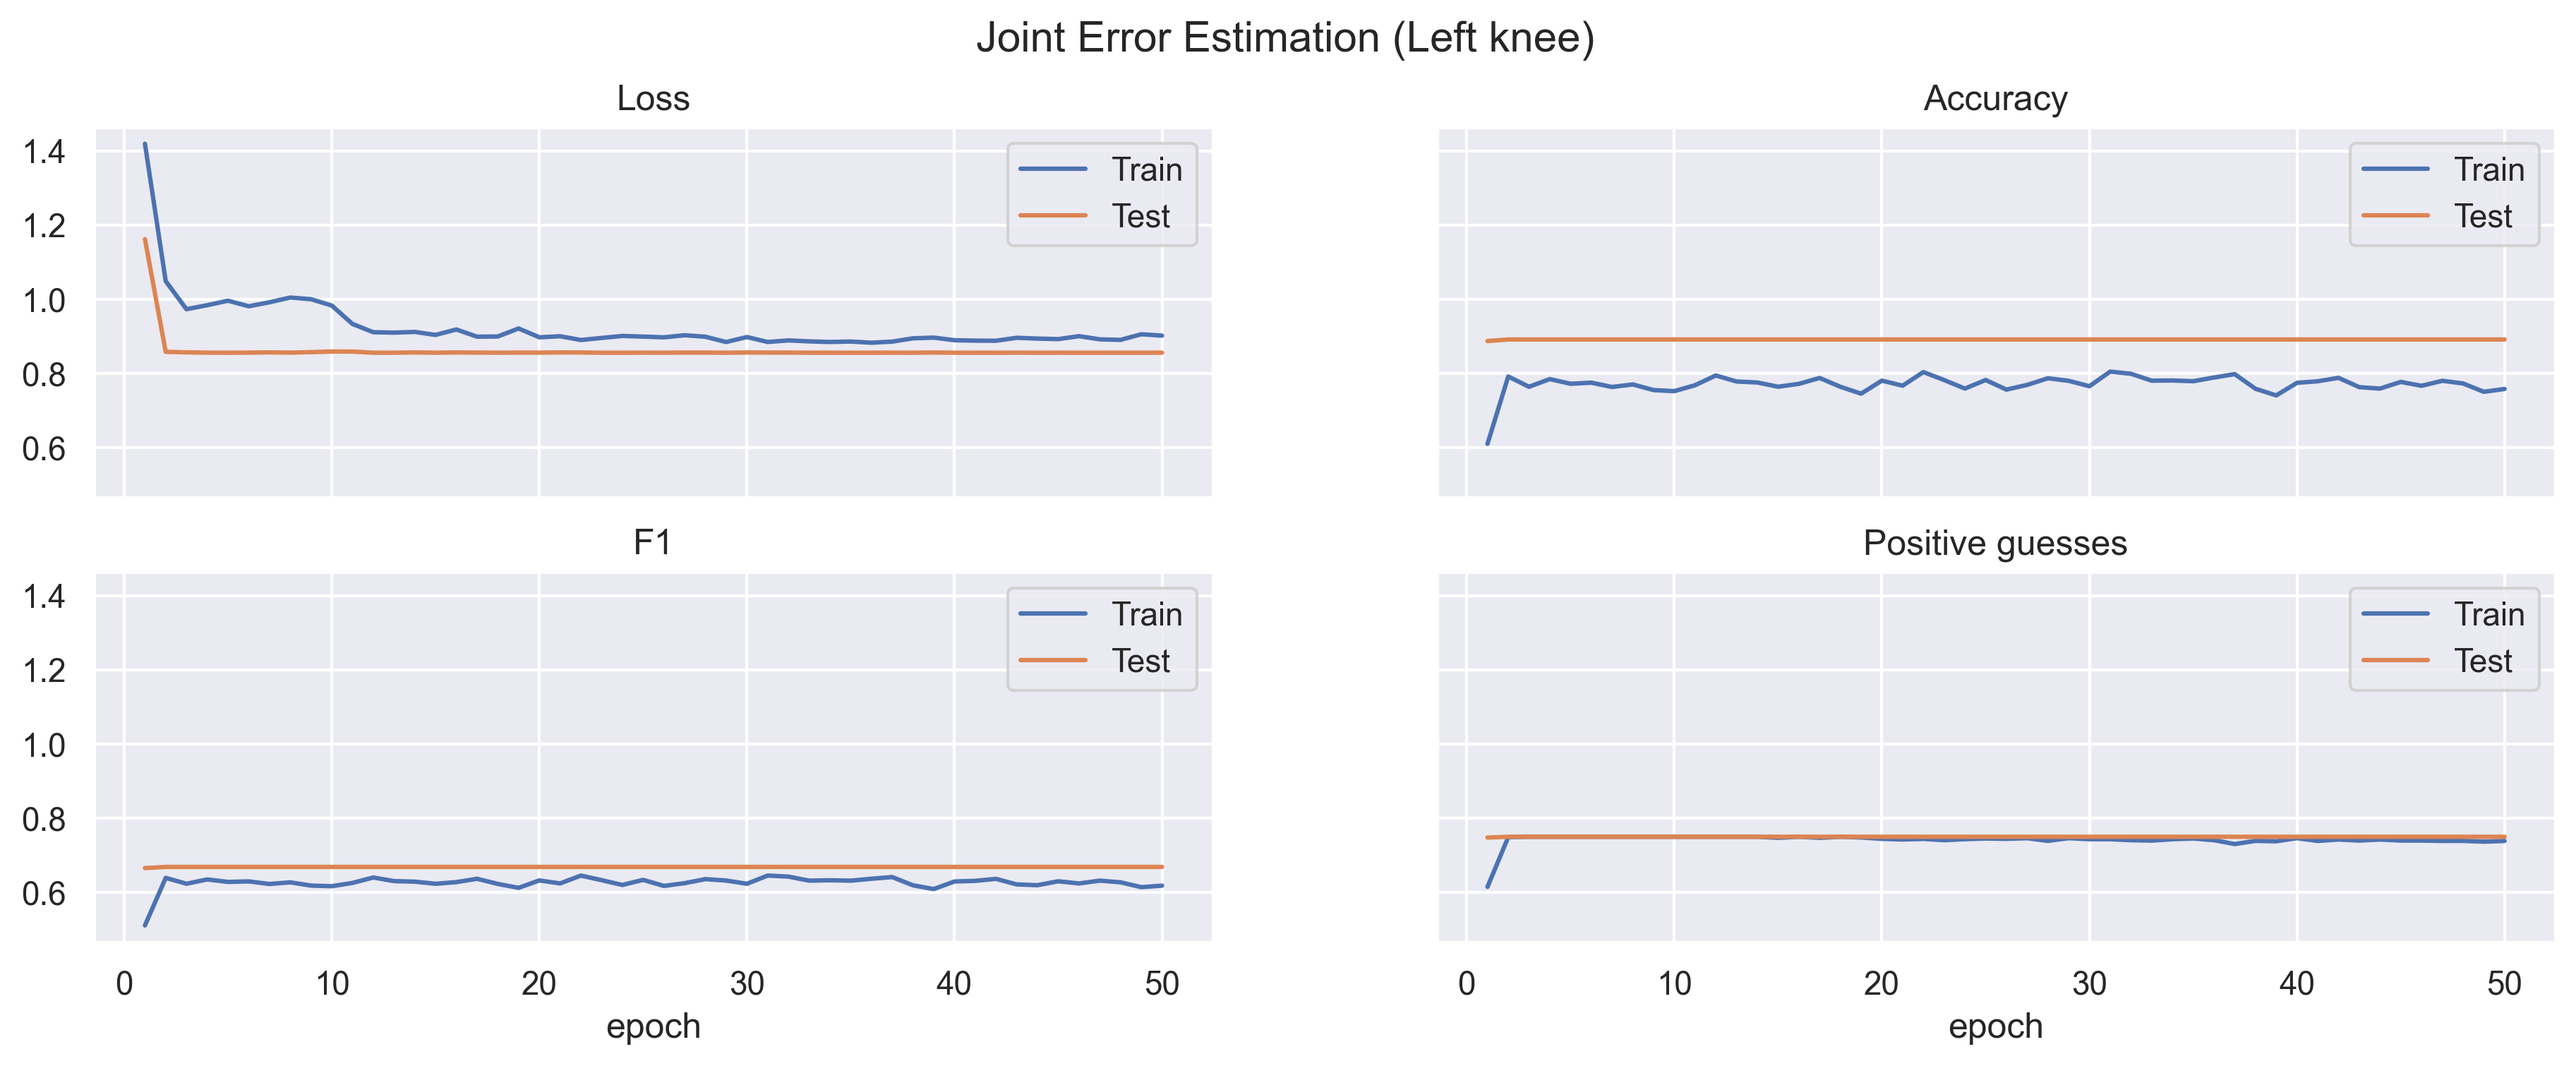
\includegraphics[width=\textwidth]{figures/Results/v1_bs_60_is_64_e_100/jt/Left knee_ErrorEstimation.png}
      \caption{left Knee Error Estimation}
      \label{fig:v1_lekn_jt_ee}
  \end{subfigure}
  \hfill
  \begin{subfigure}[b]{0.47\linewidth}
      \centering
      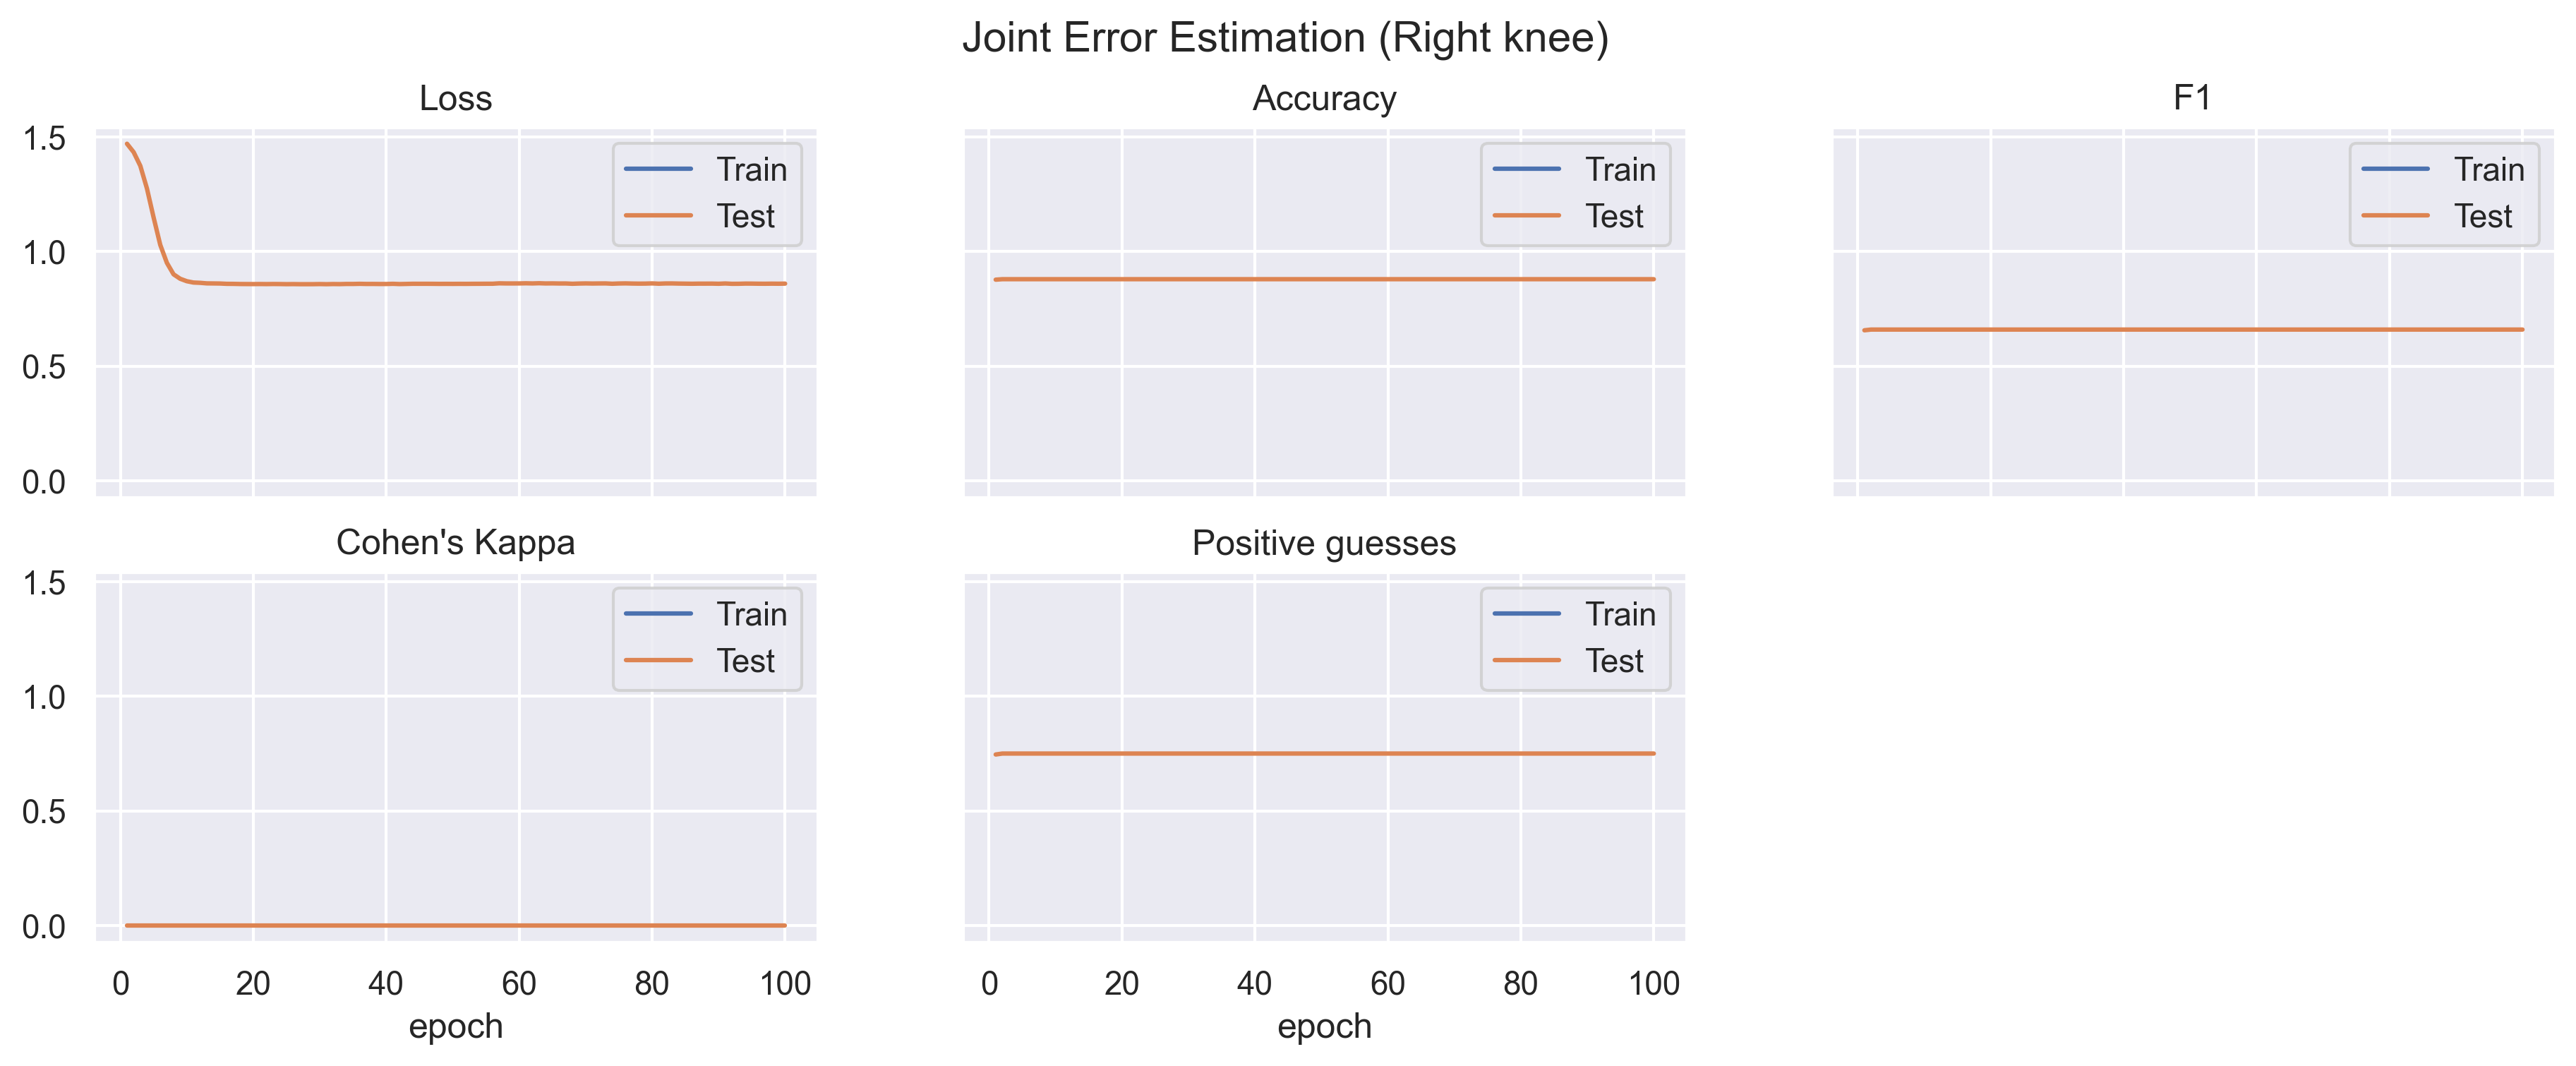
\includegraphics[width=\textwidth]{figures/Results/v1_bs_60_is_64_e_100/jt/Right knee_ErrorEstimation.png}
      \caption{Right Knee Error Estimation}
      \label{fig:v1_rikn_jt_ee}
  \end{subfigure}
  \hfill
  \begin{subfigure}[b]{0.47\linewidth}
      \centering
      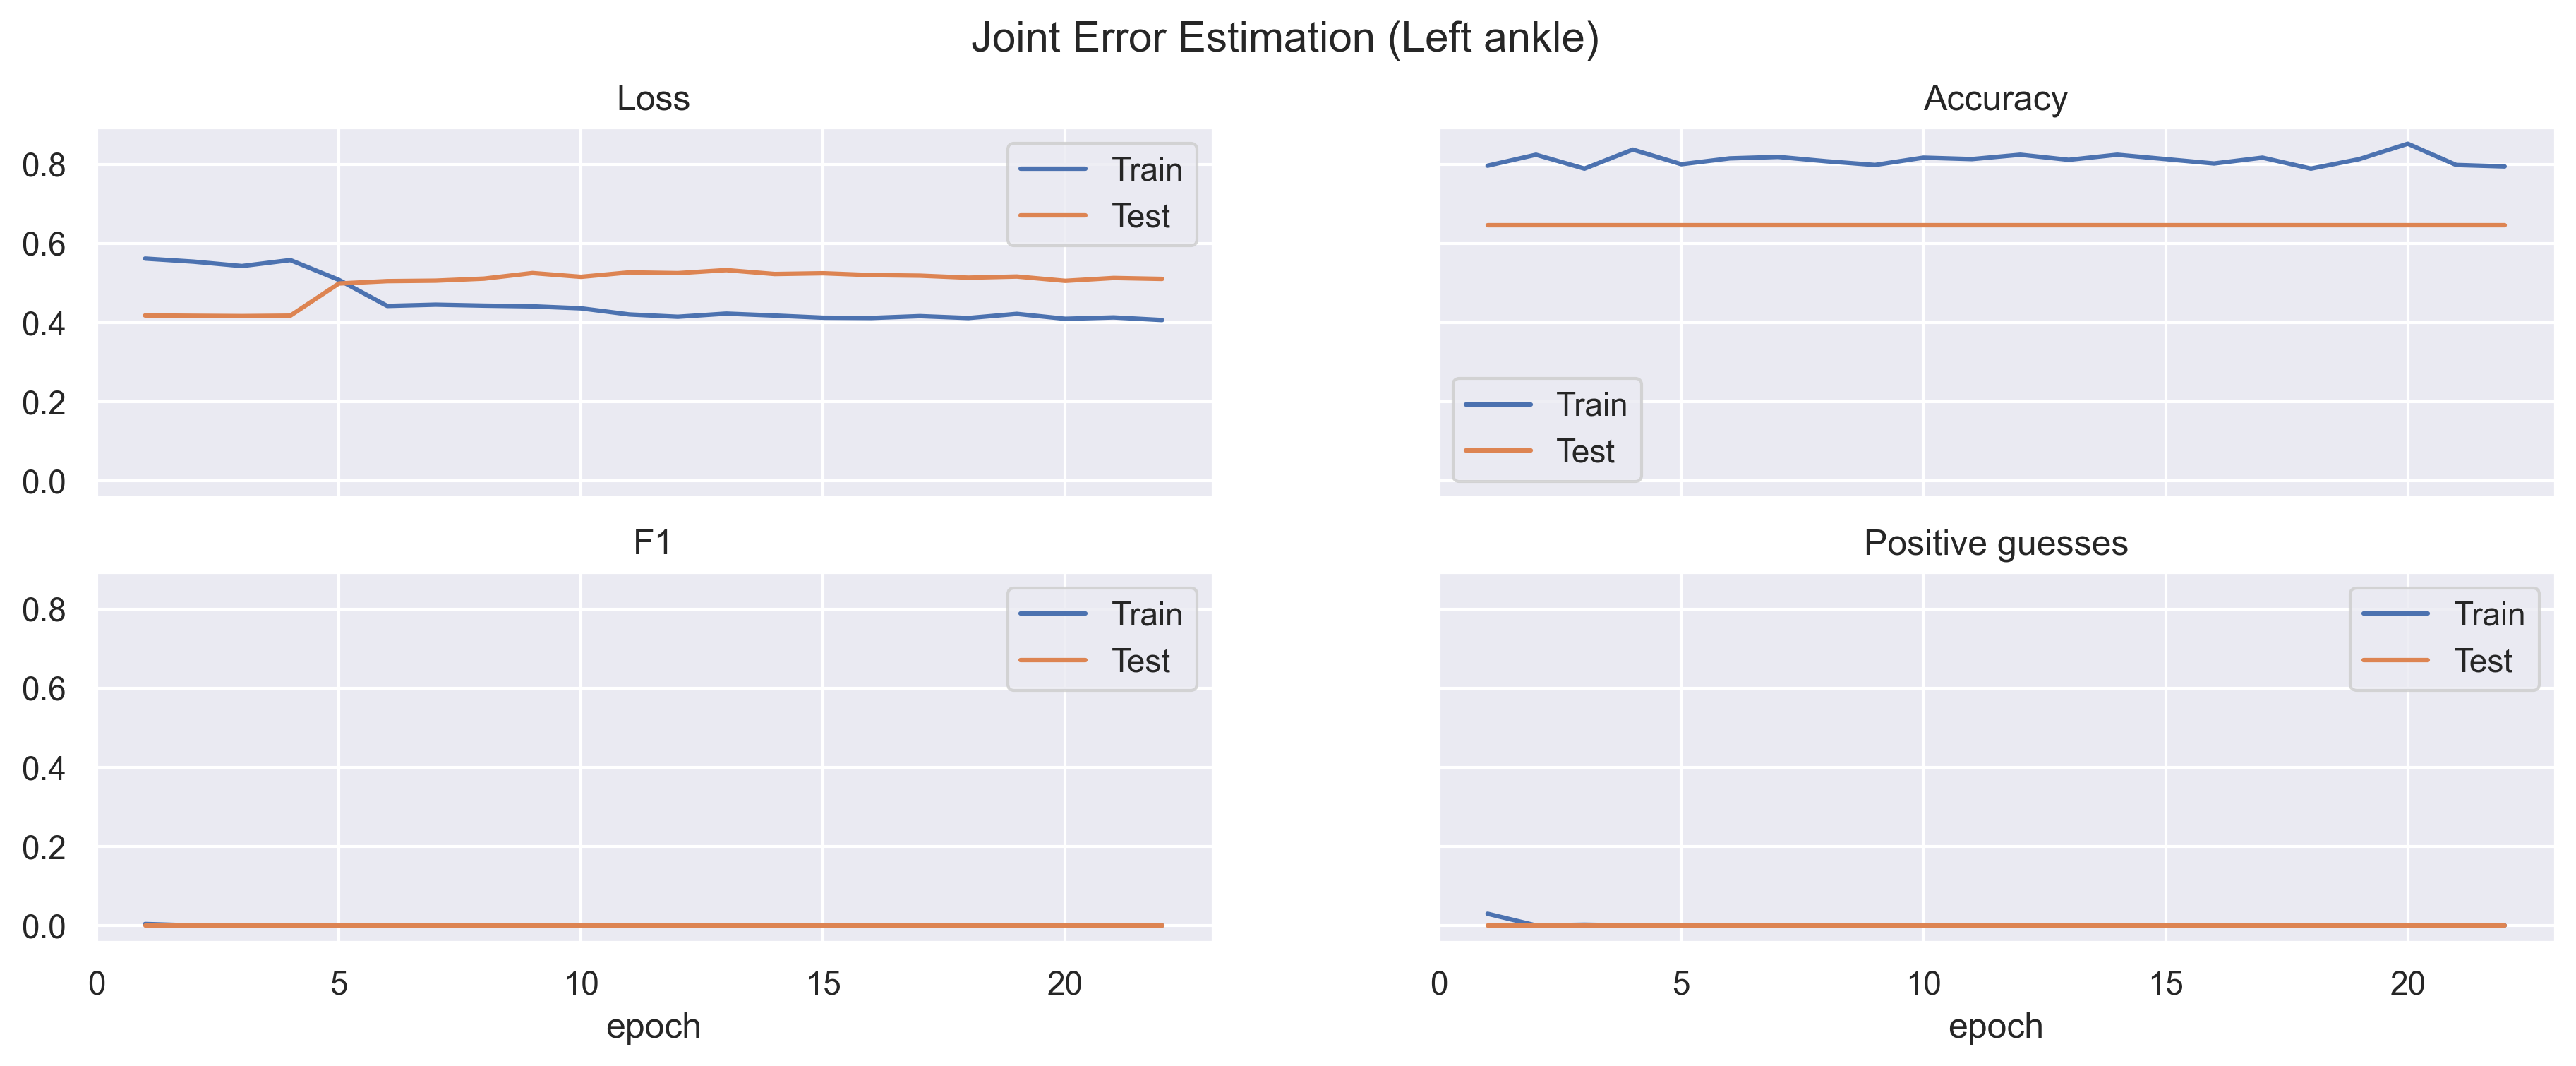
\includegraphics[width=\textwidth]{figures/Results/v1_bs_60_is_64_e_100/jt/Left ankle_ErrorEstimation.png}
      \caption{Left Ankle Error Estimation}
      \label{fig:v1_lean_jt_ee}
  \end{subfigure}
  \hfill
  \begin{subfigure}[b]{0.47\linewidth}
      \centering
      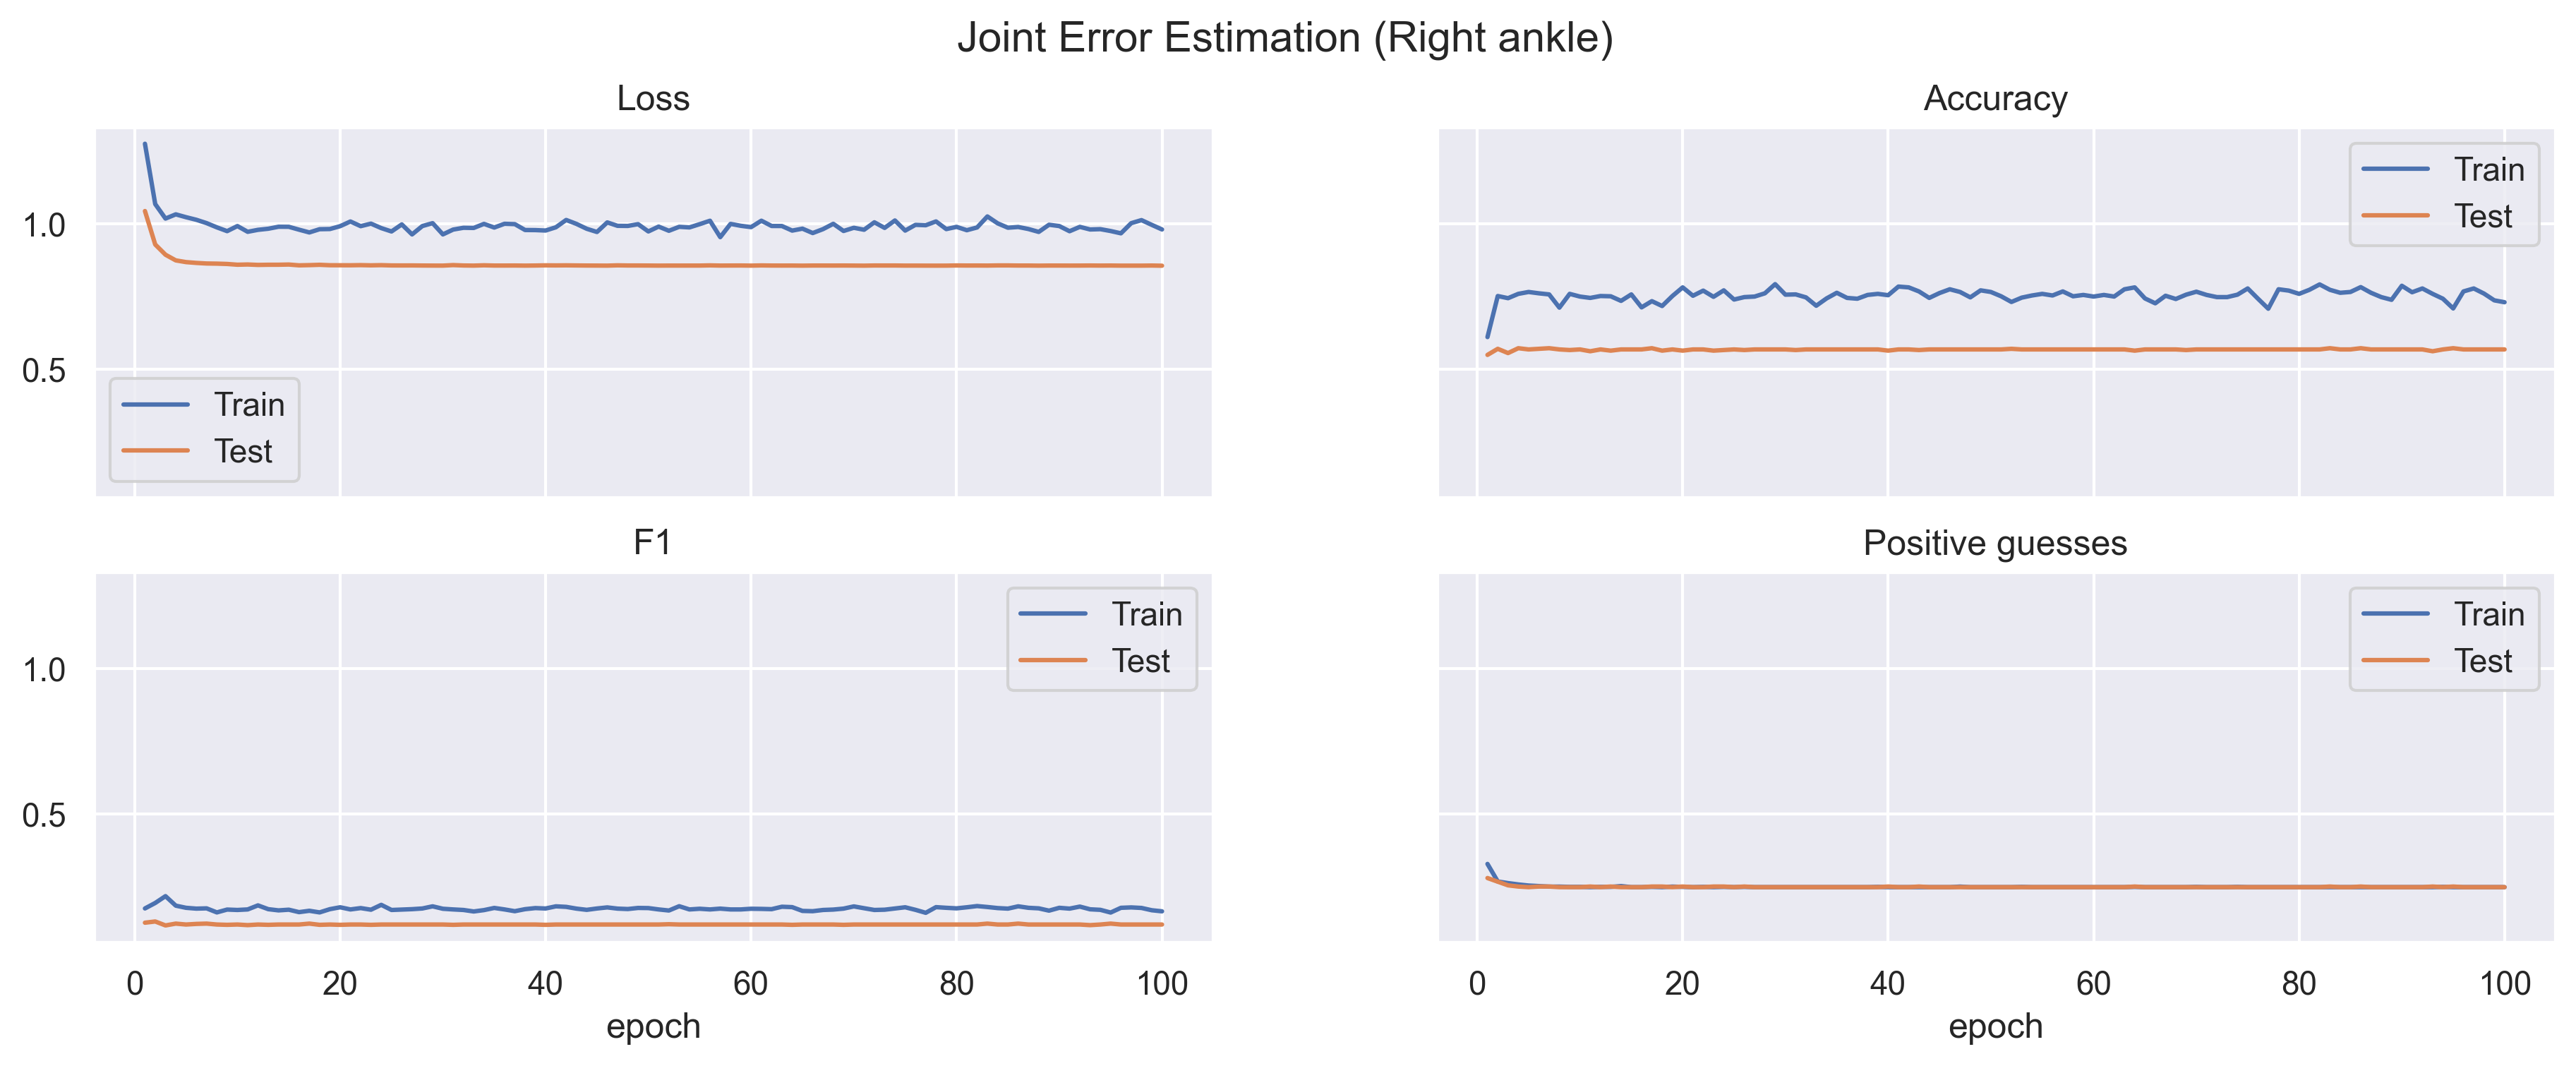
\includegraphics[width=\textwidth]{figures/Results/v1_bs_60_is_64_e_100/jt/Right ankle_ErrorEstimation.png}
      \caption{Right Ankle Error Estimation}
      \label{fig:v1_rian_jt_ee}
  \end{subfigure}
  \caption[Detailed Training results for FESDModelv2]{The training results of the Joint error estimation model for FESDModelv1.}
\end{figure}

The figures \ref{fig:conf_v1_hb}, \ref{fig:conf_v1_bp} and \ref{fig:conf_v1_jt} show the confusion matrix divided by difficulty for all four problem sets.

\begin{figure}[htbp]
  \centering
  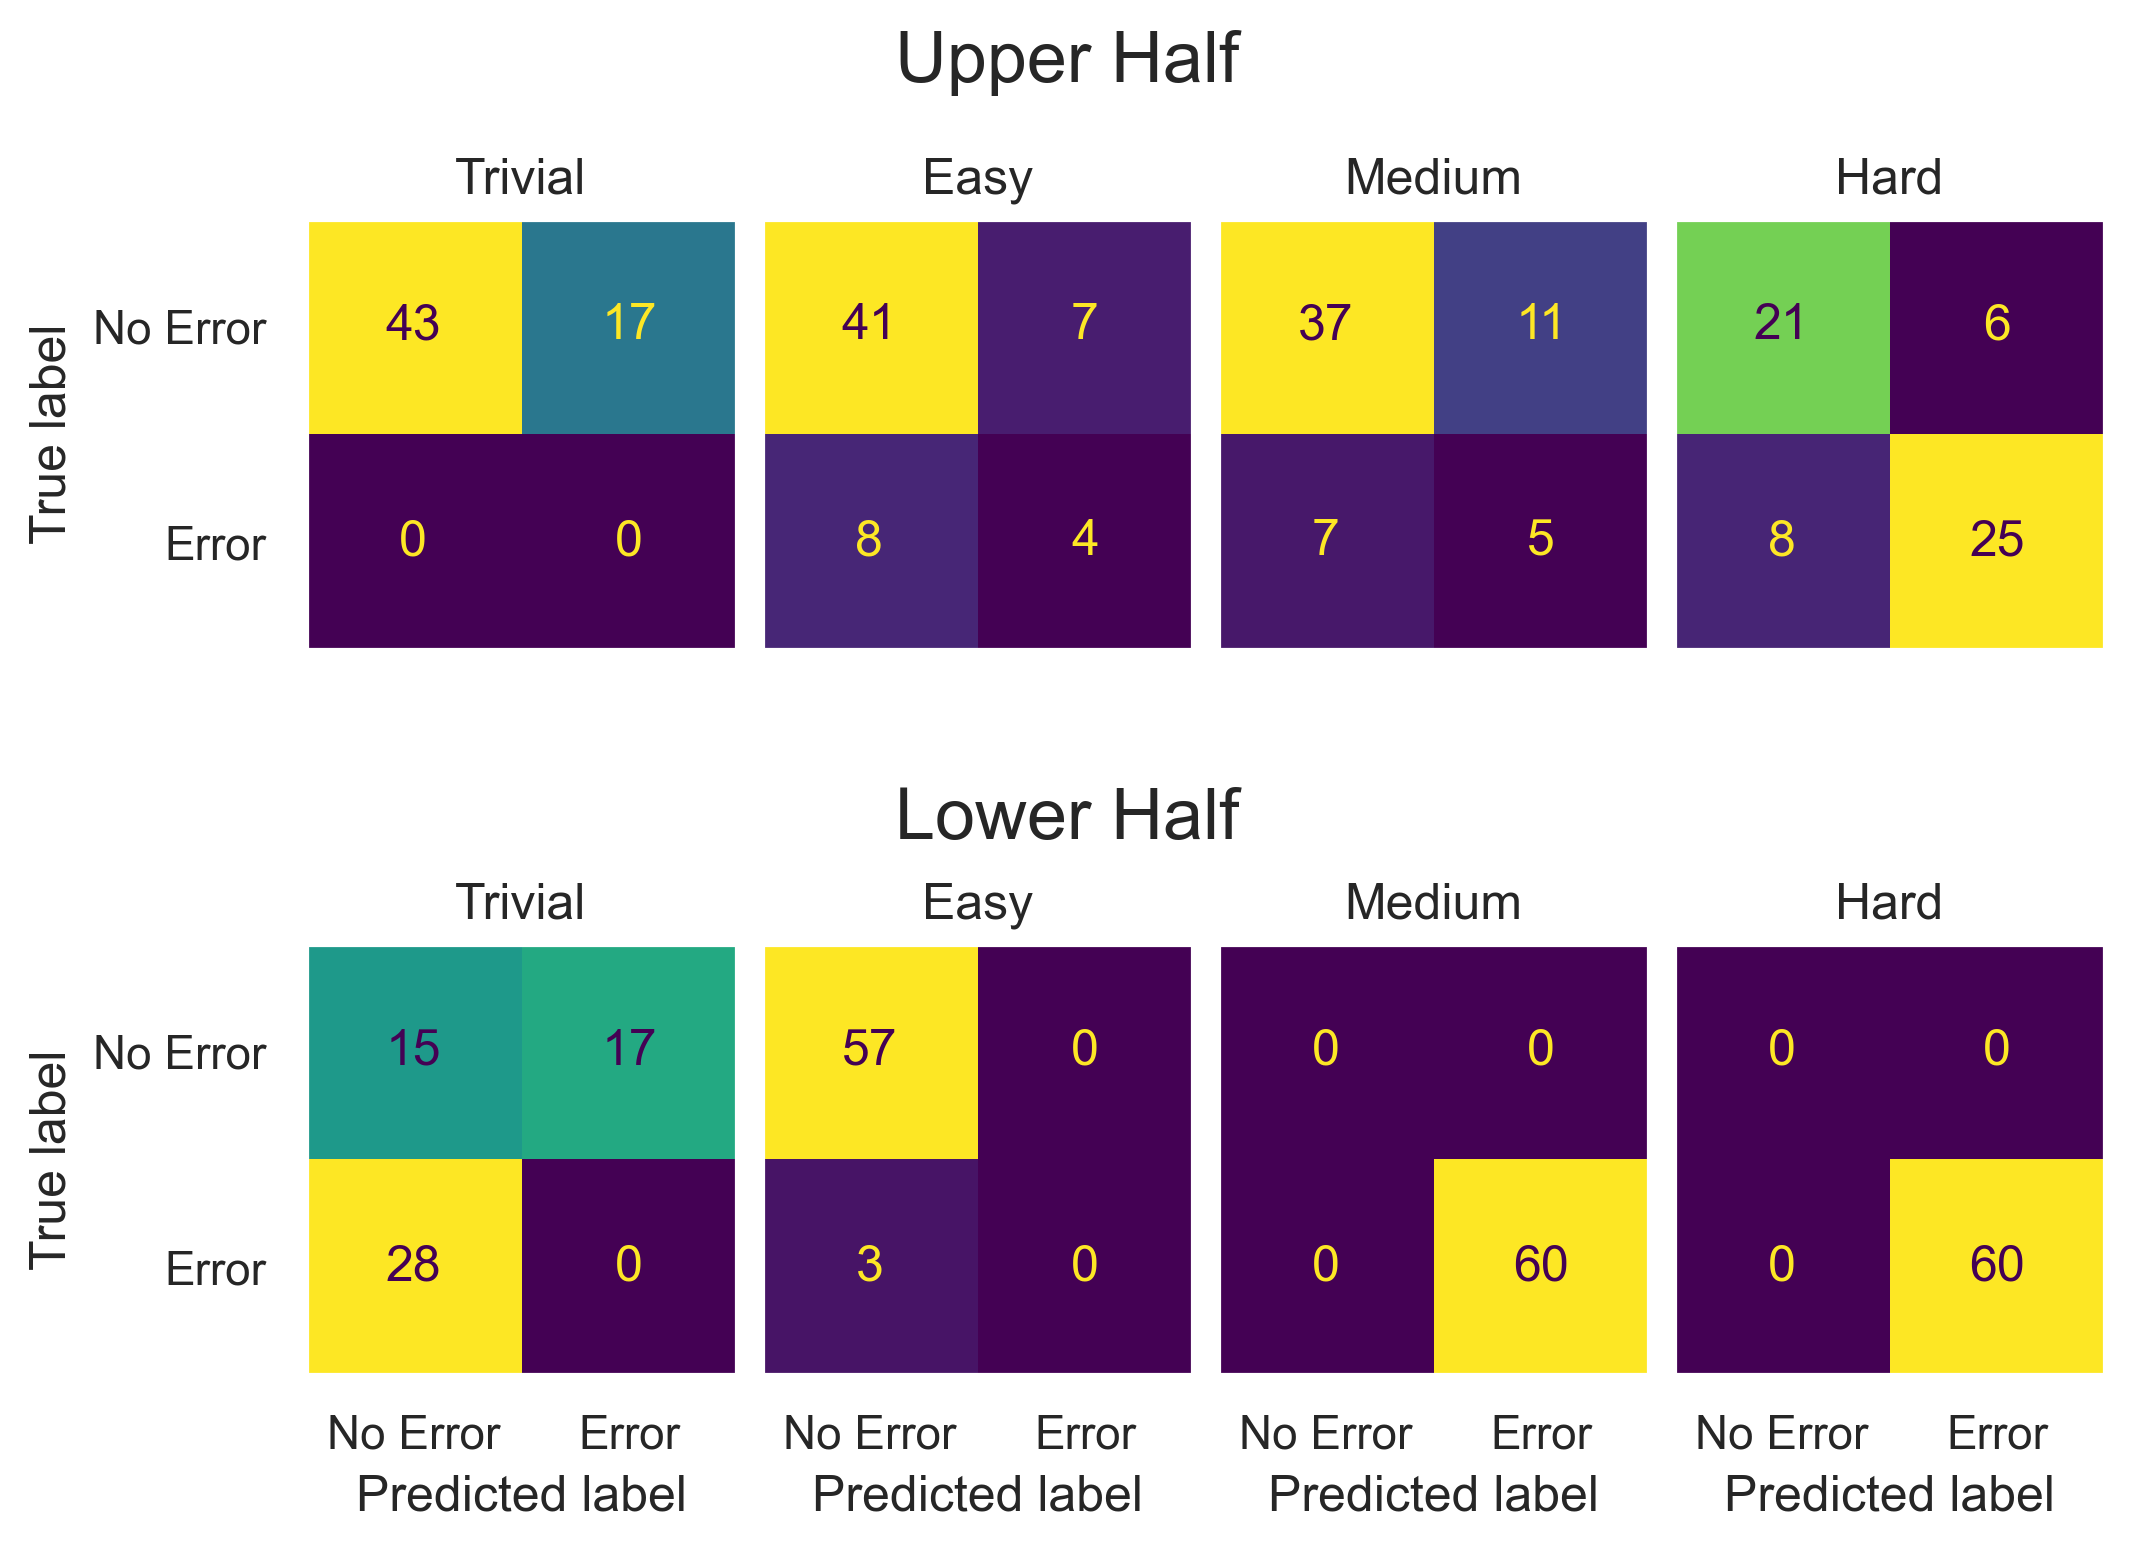
\includegraphics[width=0.8\textwidth]{figures/Results/v1/confusion/body_halves_difficulty.png}
  \caption[Full Body Confusion Matrix by Body Half and Difficulty]{The confusion matrix of the Half Body model by body half.}
  \label{fig:conf_v1_fb}
\end{figure}

\begin{figure}[htbp]
  \centering
  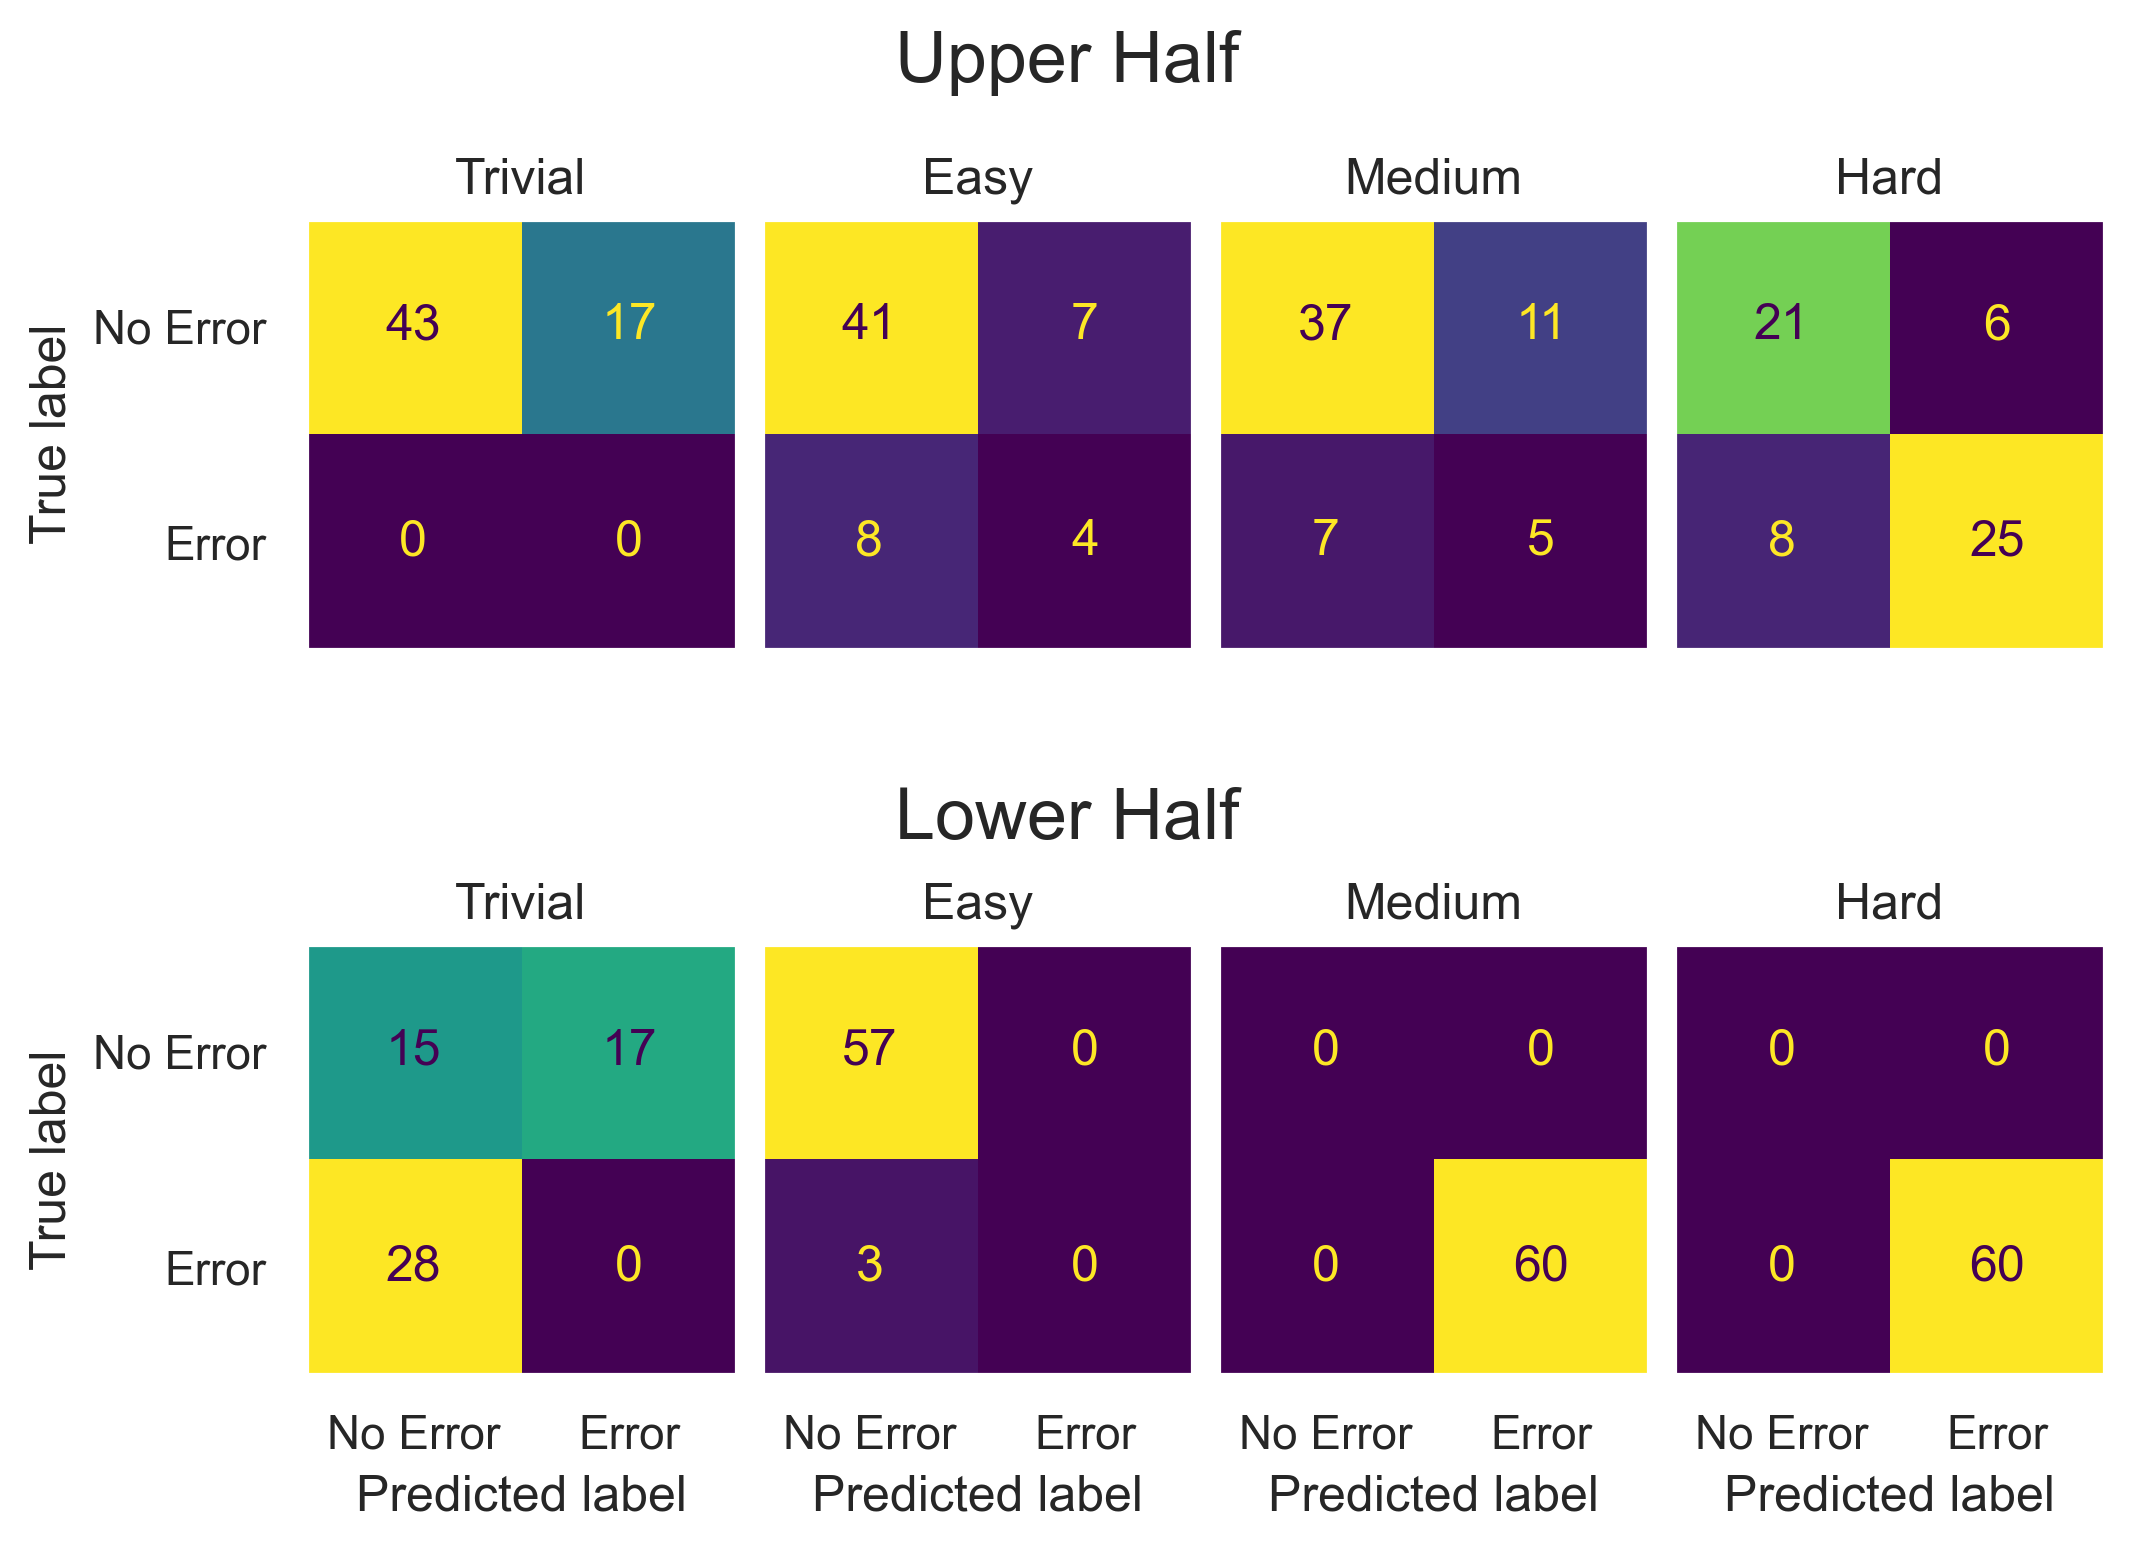
\includegraphics[width=0.8\textwidth]{figures/Results/v1/confusion/body_halves_difficulty.png}
  \caption[Half Body Confusion Matrix by Body Half and Difficulty]{The confusion matrix of the Half Body model by body half.}
  \label{fig:conf_v1_hb}
\end{figure}

\begin{figure}[htbp]
  \centering
  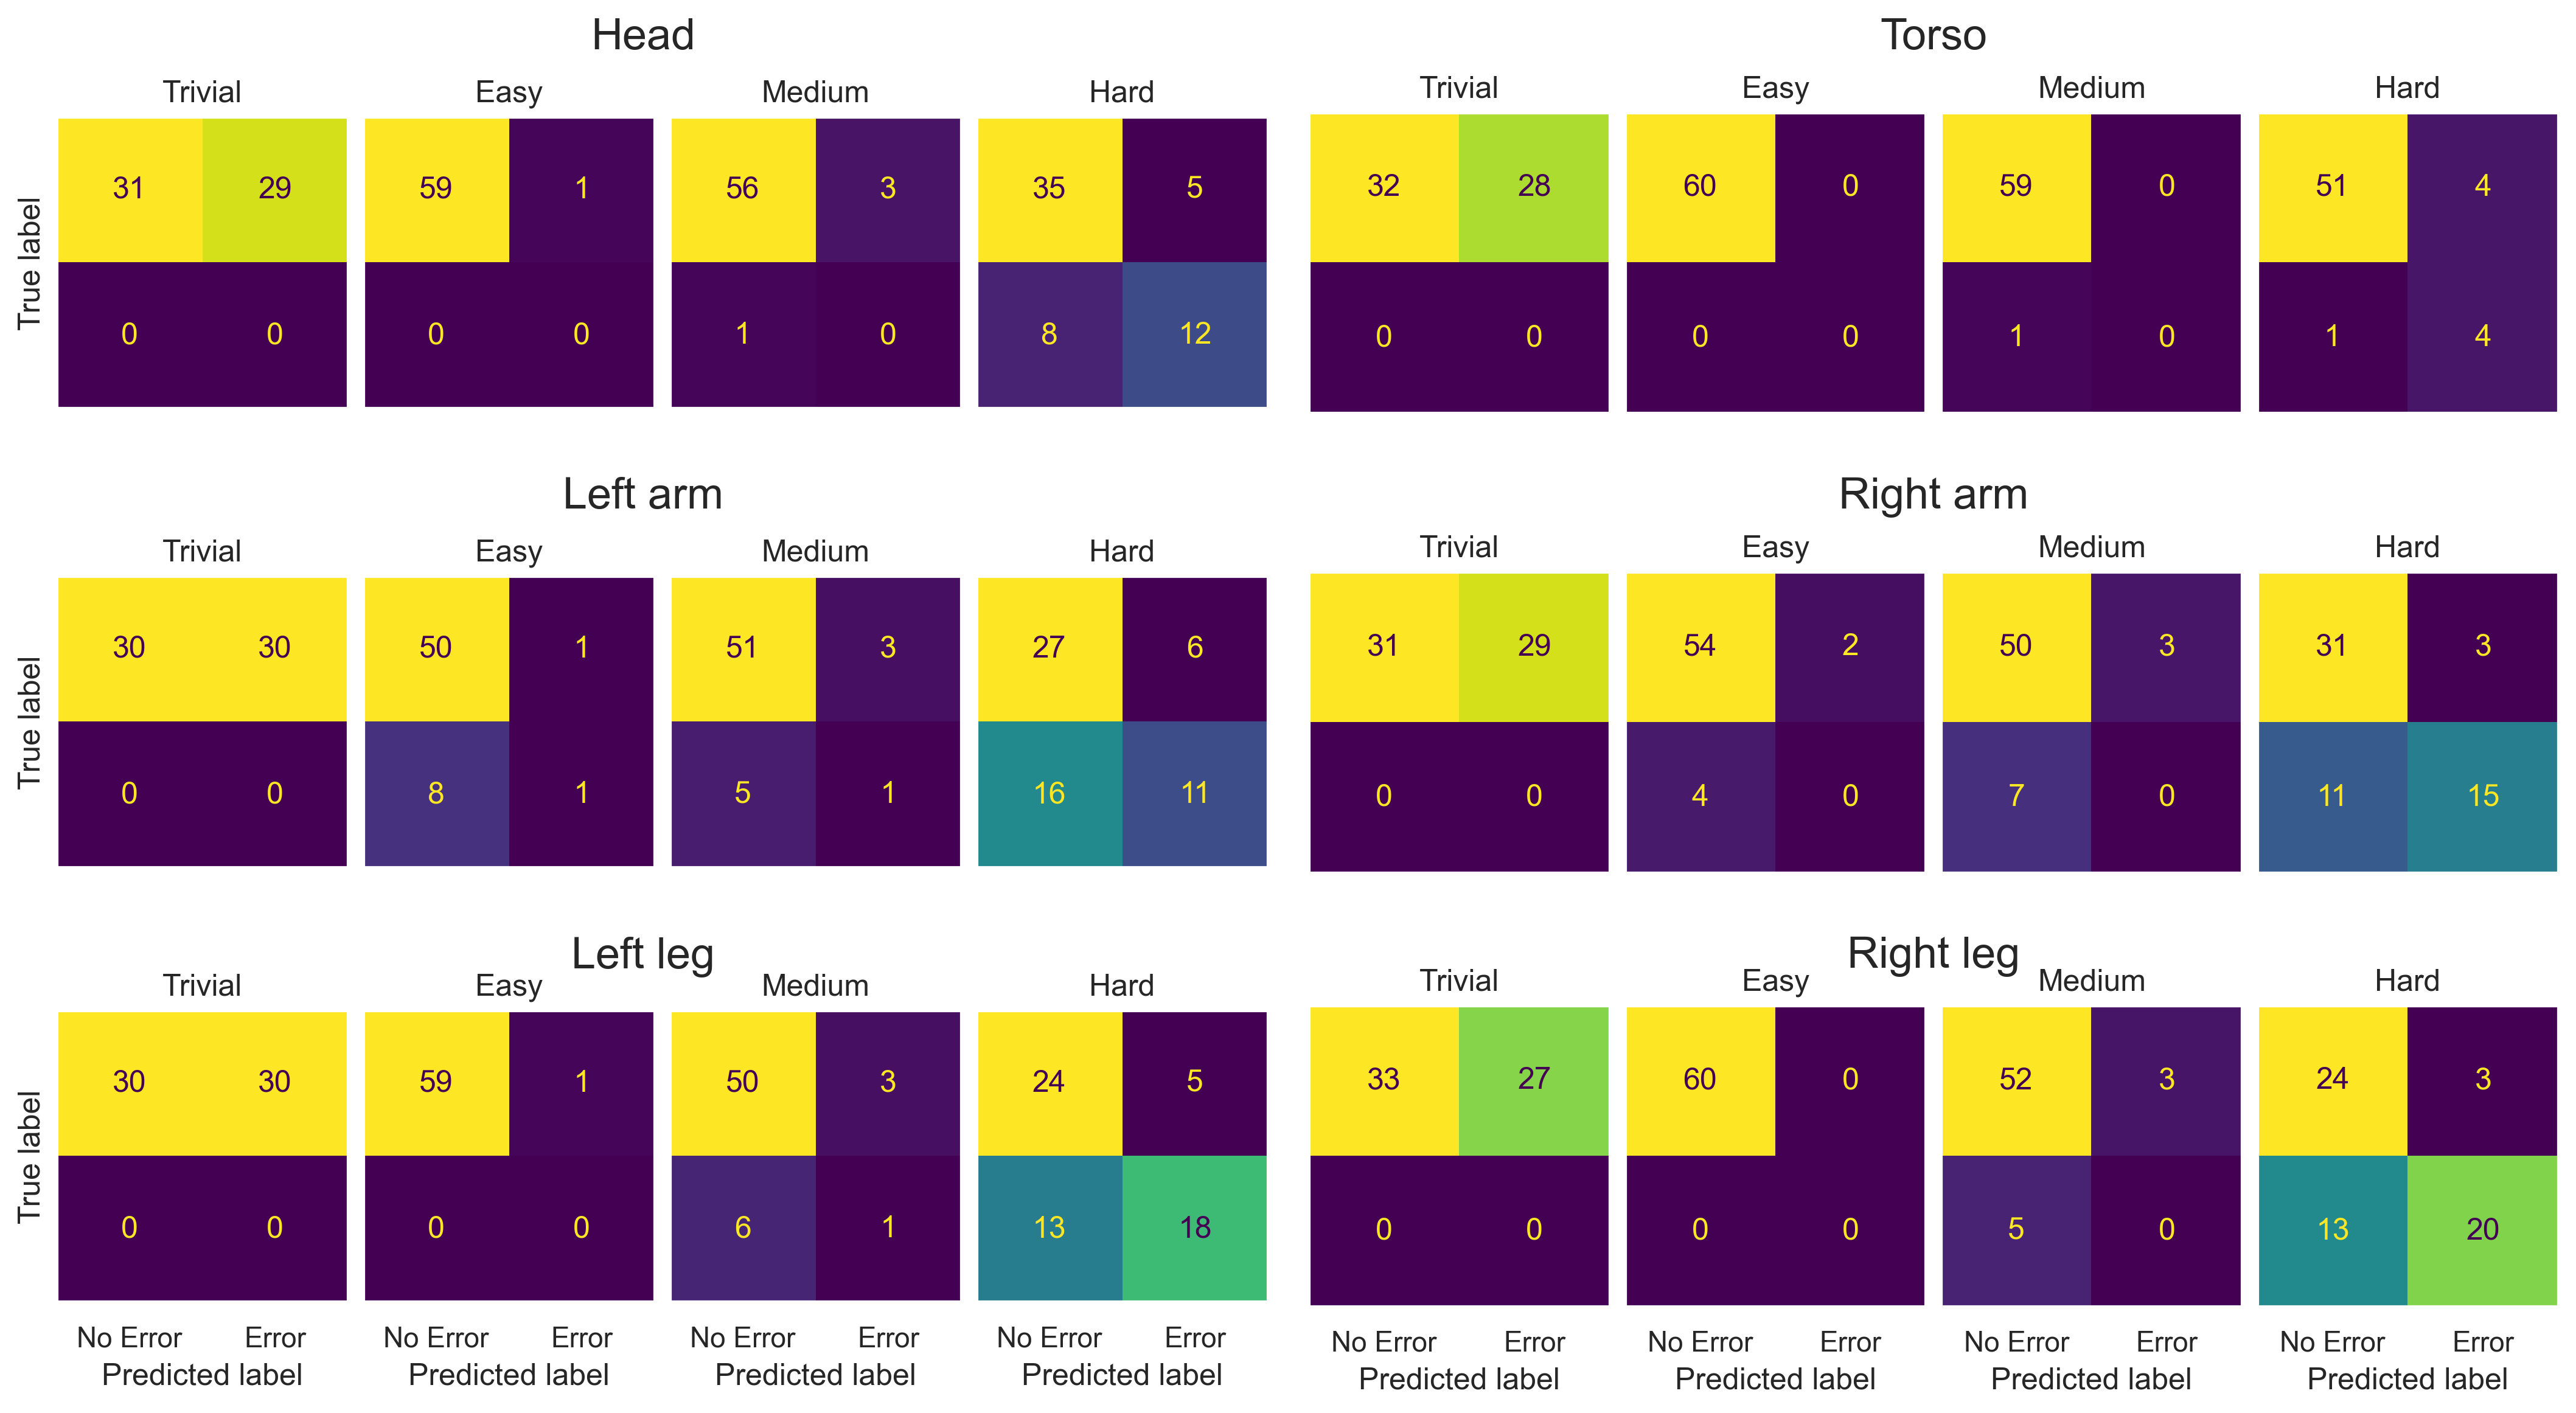
\includegraphics[width=\textwidth]{figures/Results/v1/confusion/body_parts_difficulty.png}
  \caption[Body Part Model Confusion Matrix by Body Half]{The confusion matrix of the body part model by body half.}
  \label{fig:conf_v1_bp}
\end{figure}

\begin{figure}[htbp]
  \centering
  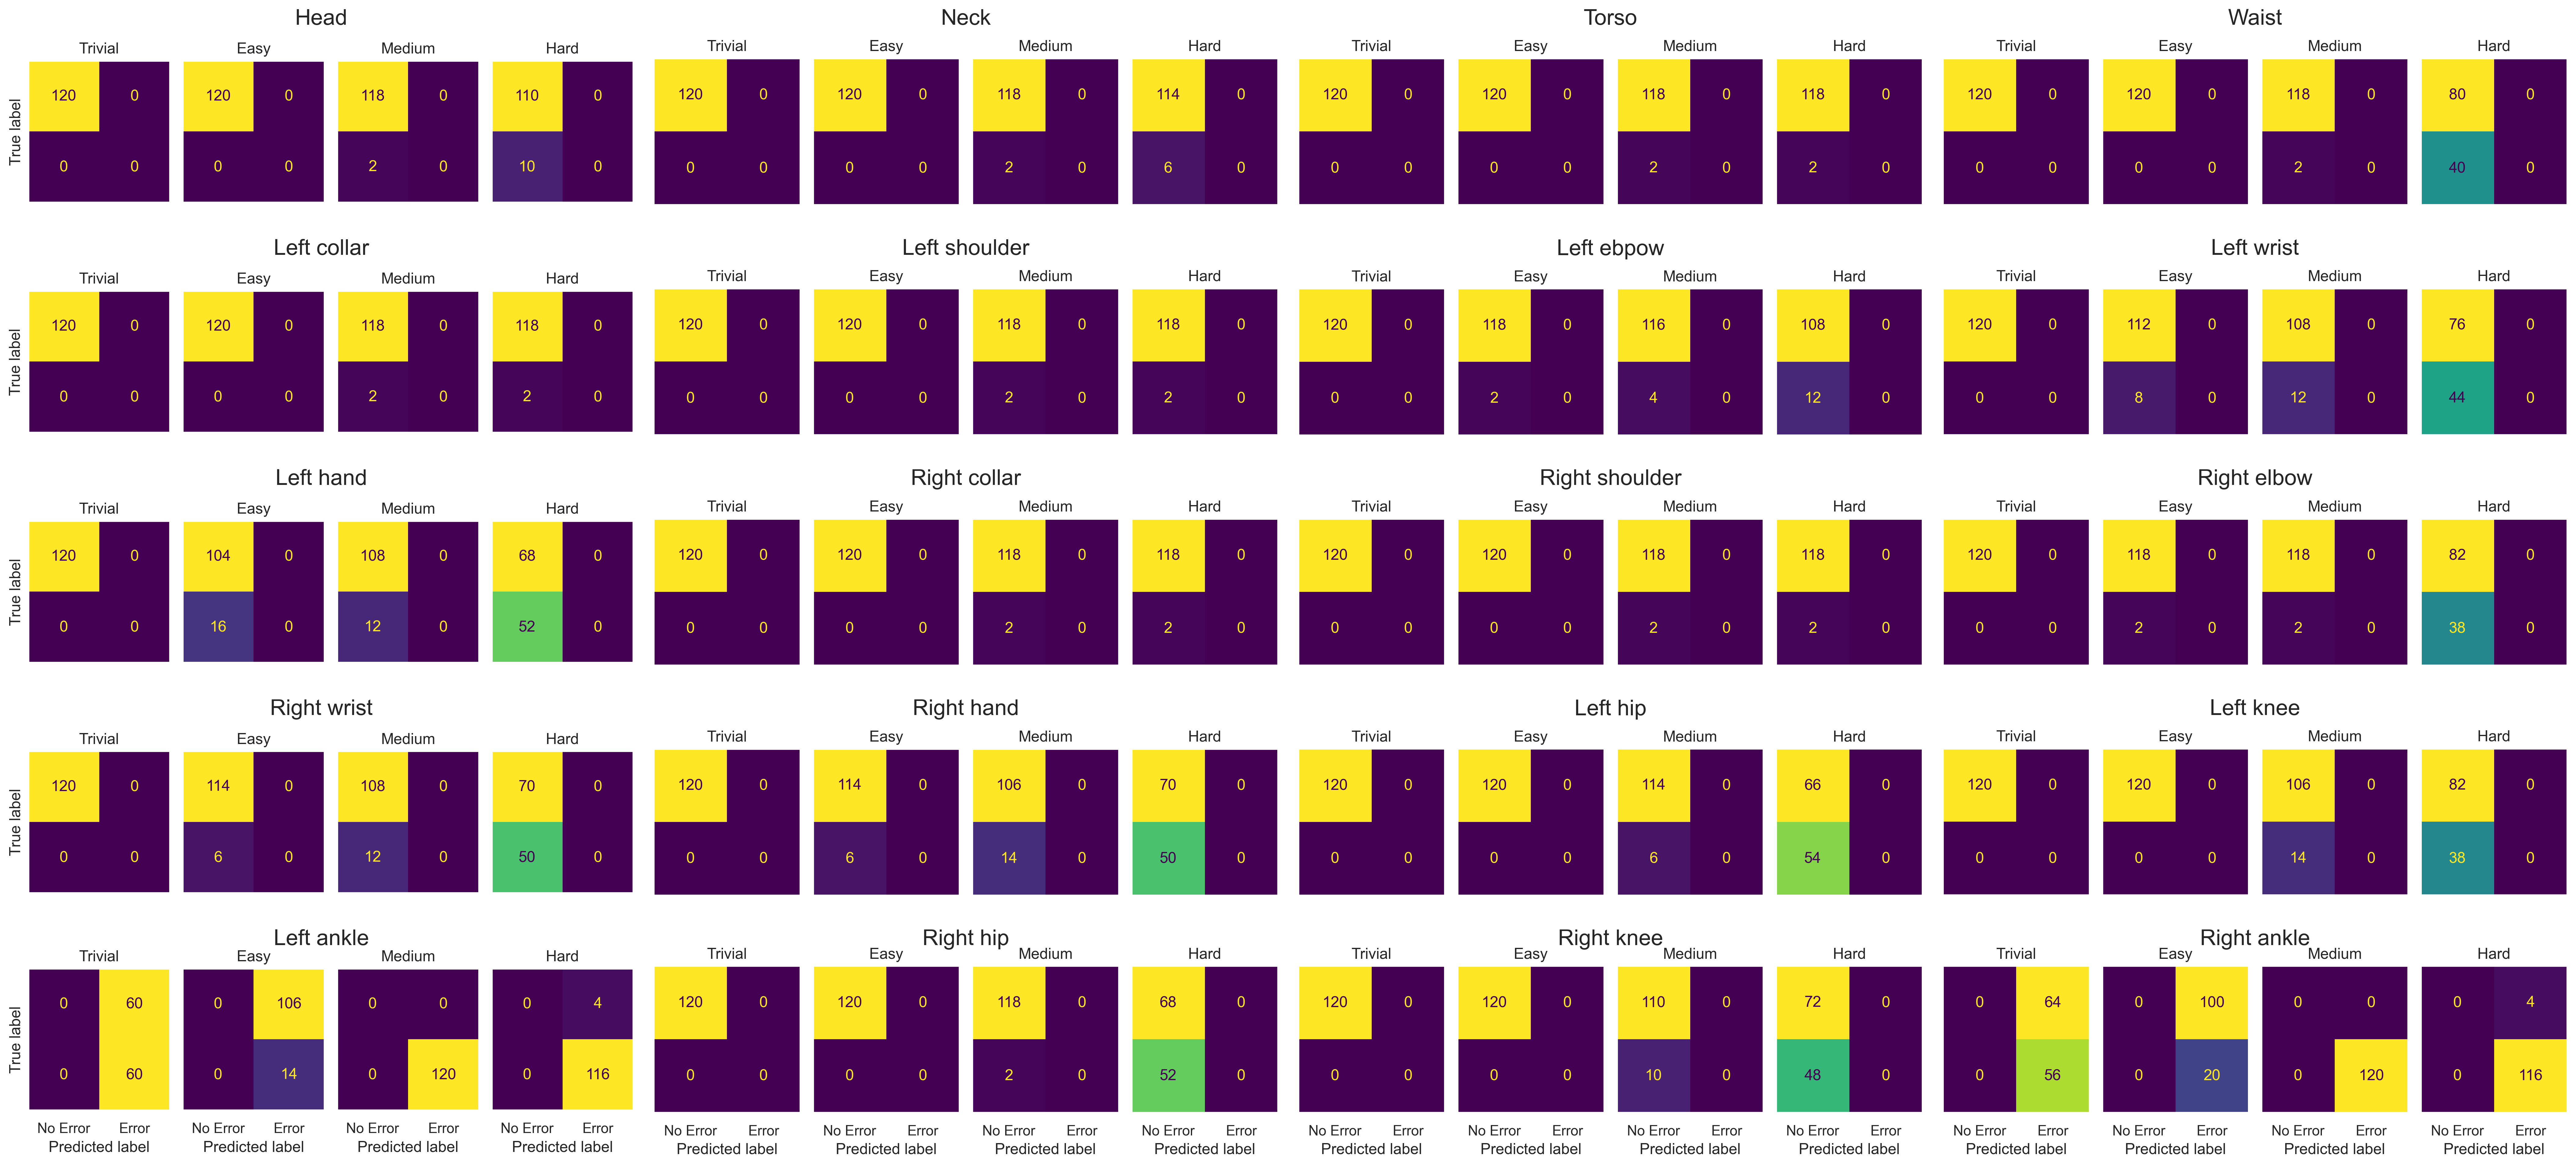
\includegraphics[width=\textwidth]{figures/Results/v1/confusion/joints_difficulty.png}
  \caption[Joint Model Confusion Matrix by Joint]{The confusion matrix of the joint model by joint.}
  \label{fig:conf_v1_bp}
\end{figure}